\chapter{The search for a low-energy excess of electron neutrinos}

\minitoc

\section{Introduction}
One of the main physics goals of the MicroBooNE experiment is to clarify the nature of the low-energy excess of $\nu_{e}$-like events observed by the MiniBooNE experiment in 2009 \cite{miniboone}. 
%The excess was found in the neutrino energy region between 200 to 475 MeV.

However, the MiniBooNE detector was a Cherenkov detector, which does not have the ability to distinguish between single electrons and single photons in the final state, making it very challenging to identify a physics model that  could definitely explain the excess.

The MicroBooNE detector, a liquid argon time projection chamber (LArTPC), provides detailed tracking and calorimetry, which allows for powerful electron/photon identification. A detailed description of the detector is available in \cite{detector}.

In this note we will describe a fully automated $\nu_{e}$ event selection in the MicroBooNE detector for the Booster Neutrino Beam (BNB) at the Fermi National Accelerator Laboratory.

\section{Signal definition}
The MiniBooNE experiment showed an excess of CCQE-like events in the 200-475~MeV neutrino energy range \cite{miniboone}, therefore this analysis will focus on a similar topology.

Our selection aims to have a sample with one electron, no other leptons or photons, at least one proton, and no other charged hadrons or mesons in the final state. All particles in the final state are required to be above detection thresholds, as defined in Section \ref{sec:eff}. These events are called $\nu_{e}$ CC0$\pi$-Np (where N > 0) \cite{teppei}.

In MicroBooNE, a $\nu_{e}$ CC0$\pi$-Np interaction corresponds to one or more ionisation tracks, produced by the protons, and an electromagnetic shower, produced by the electron. 

% This section describes the methodology of the selection
% The following sections should be here:
% - Optical Precuts
% - Optical Flash Matching
% - Cosmic Hit Removal and NuMu removal (reference marco only, really)
% - Preselection with 1+tracks, 1+showers OR 2+ showers
% - Pion and Muon Rejection in tracks (AKA, proton selection)
% - Background Rejection Cuts

\section{Analysis Methodology}
\label{sec:methodology}
The goal of the event selection is to obtain a sample enriched with $\nu_{e}$ CC0$\pi$-Np interactions. The results of the event selection are described in detail in Section \ref{sec:numu}. In order to increase the purity, two parallel background rejection strategies have been developed: one with rectangular cuts on kinematic and calorimetric variables, described in Section \ref{sec:cuts}, and one with Boosted Decision Trees, described in Section \ref{sec:bdt}.
The measurement of the systematic uncertainties affecting the variables used in the background rejection is described in Chapter \ref{sec:systematics}. The full covariance matrix has then be used to measure the sensitivity to the MiniBooNE low-energy excess signal in the electron hypothesis, in Chapter \ref{sec:sensitivity}.

\subsection{Data and Monte Carlo samples}\label{sec:data}
In this document, we will analyse a sub-sample of the data collected by the detector between February 23 and May 22, 2016. This sub-sample corresponds to an exposure of the MicroBooNE detector of \num{4.34e19} POT. This represents MicroBooNE unblinded sample for reconstruction, event selection development, and performance measurement. The sample is statistically too small to be sensitive to a MiniBooNE-like low-energy excess signal. 
%The entire dataset will be open once we are satisfied with the reconstruction, analysis chain, and future sensitivity estimates.

The data used for this analysis correspond to two separate samples: the \emph{data beam-on}, obtained with the BNB beam trigger, and the \emph{data beam-off}, obtained with the EXT trigger. These two triggers criteria were described in Section \ref{sec:trigger}.

In order to increase the simulated statistics of our $\nu_e$ CC0$\pi$-Np events, three different Monte Carlo samples were produced:
\begin{description}
\item[$\nu_{e}$ CC0$\pi$-Np + cosmic sample.] Each event has a simulated $\nu_{e}$ interaction in the MicroBooNE cryostat and simulated cosmic rays hitting the detector in the same readout window. The interaction is defined as $\nu_{e}$ CC0$\pi$-Np if it has one electron, at least one proton, no photons, and no mesons (pions, kaons) above detection threshold. The start and end points of the protons and the start point of the electron are required to be contained within the fiducial volume, as defined in Section \ref{sec:precuts}. This sample will be used to assess the reconstruction efficiencies of the analysis.
\item[BNB + cosmic sample.] Each event has a simulated neutrino interaction inside the MicroBooNE cryostat, where the neutrino flavours are weighted according to the BNB neutrino flux composition (see Section \ref{sec:beam}), and simulated cosmic rays hitting the detector in the same readout window. This sample will be used to understand backgrounds coming from other neutrino interactions.
\item[Dirt sample.] Each event has a simulated neutrino interaction outside the MicroBooNE cryostat, where the neutrino flavours are weighted according to the BNB neutrino flux composition, and simulated cosmic rays hitting the detector in the same readout window. This sample will be used to understand background events coming from interactions outside the fiducial volume.
\end{description}

Neutrino events have been generated using the GENIE Neutrino Monte Carlo generator version 2.8.6 \cite{Andreopoulos:2009rq} and cosmic rays have been generated using the CORSIKA Monte Carlo generator version 7.4003 \cite{Heck:1998vt}. Simulated secondary particle propagation employs GEANT version 4.9.6 \cite{Brun:1994aa}, and detector response simulation and reconstruction is performed with the LArSoft framework version 6.26.01.10 \cite{Church:2013hea}.

\subsection{Overview of the analysis}
The reconstruction and selection chain to identify $\nu_{e}$~CC0$\pi$-Np electron neutrino candidate events for this analysis is divided into several stages:

\begin{description}
\item[Cosmic-ray removal.] In order to suppress the cosmogenic background, the first step is to rune the Pandora algorithms optimised to reconstruct and remove cosmic rays \cite{Acciarri:2017hat}. After this step, hits associated with objects deemed as cosmic-induced by several tagging algorithms, external to Pandora and described in Section \ref{sec:cosmicremoval}, are removed from the event. The remaining hit collection provides the input to the Pandora neutrino reconstruction path, which outputs a list of candidate neutrinos.

\item[Optical selection.] A minimum amount of coincident photoelectrons in the optical detection system is required to be coinciding with the BNB beam window and at least one of the neutrino candidates provided by the Pandora framework must be compatible with the flash observed in the optical detection system. These requirements are described in detail in Section \ref{sec:optical_pre_cuts}.

\item[Electron neutrino topological pre-selection.] One of the neutrino candidates must be compatible with the topology of a $\nu_{e}$ CC0$\pi$-Np interaction. Rather than accepting strictly $N$ tracks and one shower, at least one track and at least one shower or at least two showers sharing a common vertex are accepted, due to the presence of split showers and split tracks. Multiple showers without reconstructed tracks are accepted due to a current track/shower identification inefficiency, addressed in Section \ref{sec:ineff}.

\item[CC $\nu_{\mu}$ neutrino candidates removal.] Events tagged as CC $\nu_{\mu}$ neutrino candidates are rejected by an independent CC $\nu_{\mu}$ selection module, described in \cite{ubxsec}. 

\item[Calorimetric variables reconstruction.] The energy of the electron showers is measured with a calorimetric procedure, converting the collected charge into deposited energy, while the energy deposited by the proton tracks is calculated from the length of the reconstructed track. The $dE/dx$ of the ionisation tracks and electromagnetic showers is also measured for particle identification purposes and are detailed in Section \ref{sec:energyreco}.

\item[Background rejection.] The $\nu_{e}$~CC0$\pi$-Np events can be further isolated by applying a suite of cuts on kinematic, geometric, and calorimetric variables. The electromagnetic showers initiated by an electron in the final state are isolated with a cut on the $dE/dx$ value and the proton tracks are selected with a cut on the $\chi^{2}$ score of their $dE/dx$ vs. residual range profile. An alternative background-rejection strategy has also been developed using Boosted Decision Trees. These are described in Sections \ref{sec:cuts} and \ref{sec:bdt}.
\end{description}

A schematics of the event selection stages is shown in Figure \ref{fig:selection}.

\begin{figure}[htbp]
\centering
  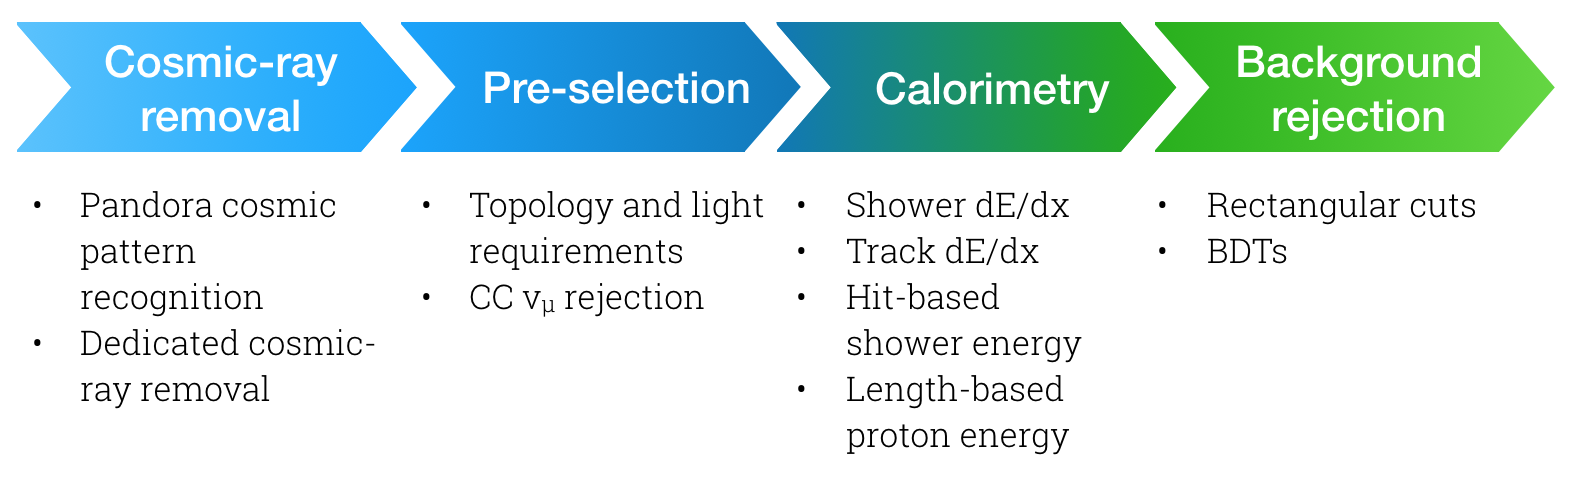
\includegraphics[width=0.9\linewidth]{figures/selection.png}
  \caption{Schematics of the $\nu_e$ CC0$\pi$-Np event selection stages, from the cosmic-ray removal to the rejection of the neutrino and cosmogenic backgrounds.}
  \label{fig:selection}
\end{figure}

\subsection{Cosmic-ray rejection}\label{sec:cosmicremoval}
The hits in the TPC, reconstructed with the procedure described in Section \ref{sec:eventreco}, are passed to the Pandora framework for pattern recognition. %The framework can run in two different modes: one optimised for the reconstruction of cosmic rays and delta rays (\emph{cosmic mode}), and one optimised for the reconstruction of neutrino interactions (\emph{neutrino mode}).

In order to reject the cosmogenic background, Pandora is first run in cosmic mode over all the reconstructed hits. This reconstruction is track-oriented, and the delta rays are reconstructed as showers and considered as daughters of the closest cosmic muon. The starting point of the reconstructed tracks in this mode is assumed to be the highest $y$ coordinate \cite{Acciarri:2017hat}.
These reconstructed high-level objects are fed to a series of cosmic-ray tagging algorithms, which are briefly described below.
\begin{description}
\item[Geometry and timing algorithm.] This algorithm checks if the reconstructed hits have a time compatible with the drift-time window. If a track or a shower has more than four hits outside the allowed drift-time window, then they are tagged as cosmic rays. Then, the algorithm loops over all the reconstructed objects and tag them if they have a trajectory that enters and exits the TPC borders, within a fiducial volume. The fiducial volume has been chosen by taking into account the magnitude of the space charge effect (Section \ref{sec:ionisation}).
\item[Flash-matching algorithm.]{This algorithm takes into account the information provided by the optical system to reject cosmic rays interacting during the readout window. The algorithm first requires the presence of a reconstructed flash during the beam-spill window of 1.6~\si{\micro}s. Then, for each reconstructed particle a \emph{flash hypothesis} is built, meaning that we create a distribution of the light collected by each PMT compatible with the charge distribution of the reconstructed particle. The reconstructed particle is tagged as a cosmic ray if its hypothetical flash satisfies two requirements:
\begin{enumerate}
    \item at least one PMT sees an amount of PE $3\sigma$ larger than the amount of PE in the flash hypothesis in the same PMT.
    \item the $z$ coordinate of the flash hypothesis is not compatible with the $z$ coordinate of the flash observed.
\end{enumerate}}
More details can be found in Section \ref{sec:optical_pre_cuts}.

\item[Anode-Cathode Piercing Tracks algorithm.] The coordinate along the drift direction (which in MicroBooNE is the $x$ coordinate) can be reconstructed in a LArTPC only by knowing also the time $t$ when the particle interacted in the detector. The $x$ coordinate is then given by:
\begin{equation}
    x = v_{\mathrm{drift}}t,
\end{equation}
where $v_{\mathrm{drift}}$ is the drift velocity. In the case of a neutrino interaction, the time $t$ correspond to the beam trigger (plus a definite interval), while for a cosmic ray cannot be known without an external cosmic-ray tagger.
However, for the subset of cosmic rays piercing the cathode (or the anode) we will have:
\begin{align}
    t_{S(E)} - t_F \sim t_{C(A)},\label{eq:acpt}
\end{align}
where $t_S$ ($t_E$) is the time of the track start point (end point), $t_F$ is the time of the flash corresponding to the track, and $t_C$ ($t_A$) is the time corresponding to the position of the cathode (anode). Thus, for each track we loop over all reconstructed flash and we consider the track of cosmic origin if there is a flash which satisfies condition \ref{eq:acpt}.

\item[Stopping-muon algorithms.] Cosmic muons which enter the TPC and stop in the liquid argon are caused by muons which decayed to a Michel electron while in the TPC. They can be reconstructed as a track (the cosmic muon) and a shower (the Michel electron). Figure \ref{fig:michel_evd} shows a data event display of the collection plane with a stopping muon.

\begin{figure}[htbp]
\centering
  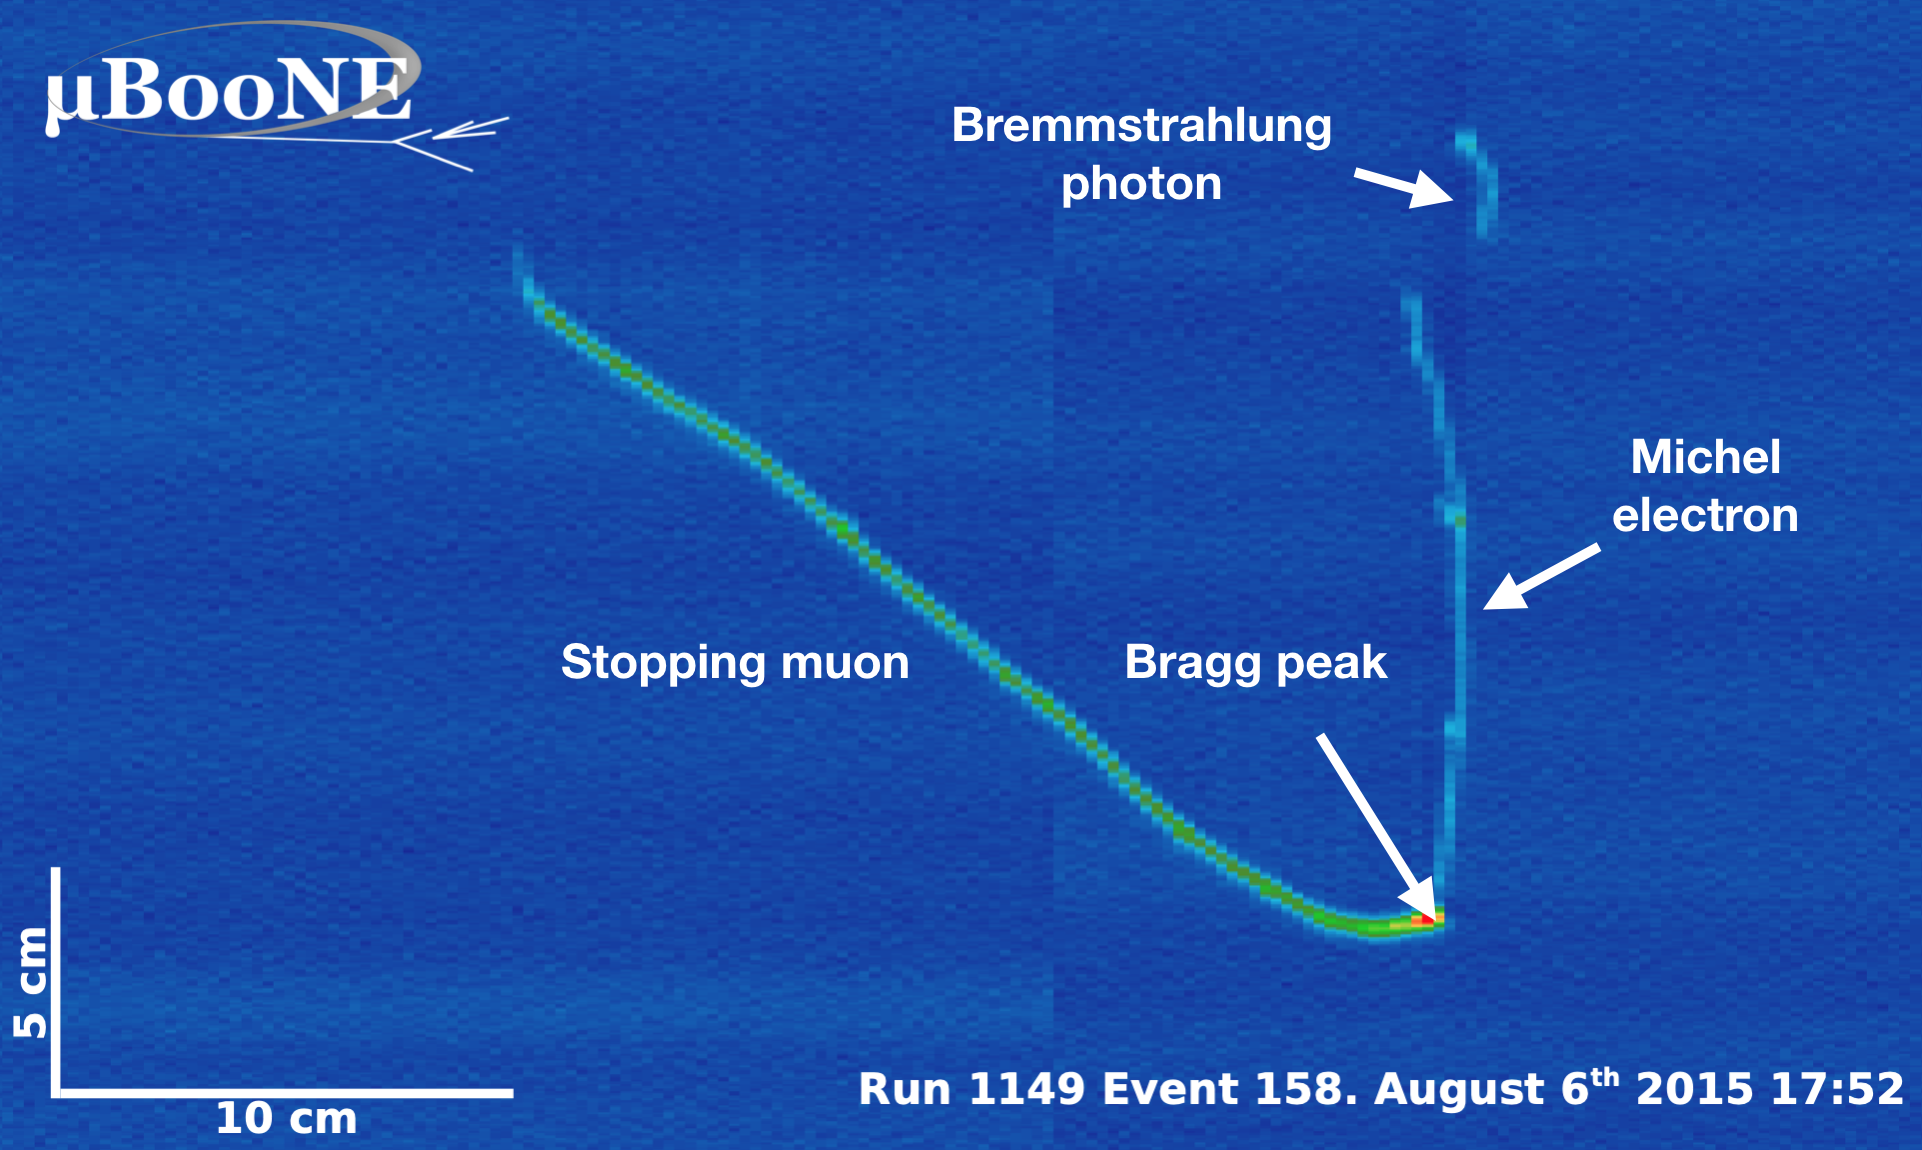
\includegraphics[width=0.75\linewidth]{figures/michel_evd.png}
  \caption{Event display of the collection plane with a muon stopping and decaying, producing a Michel electron.}
  \label{fig:michel_evd}
\end{figure}

This topology is similar to the one of an electron neutrino interaction. For this reason, stopping muons represent an important background for our analysis. 
They are tagged in two ways:
\begin{itemize}
    \item a series of pattern recognition and calorimetric algorithm try to identify the correct direction of the cosmic muon track (by measuring its energy loss profile) and to verify the presence of a \emph{kink} in the trajectory, caused by the presence of the Michel electron.
    \item the multiple Coulomb scattering (MCS) angle of a stopping muon will increase as its momentum decrease, while for through-going muons it is essentially constant \cite{Abratenko:2017nki}. By fitting the track profile with the MCS hypothesis in both direction (up-going and down-going), it is possible to verify if the cosmic muon is stopping in the detector. 
\end{itemize}

\end{description}

The hits associated with the tagged reconstructed objects (and to their daughters) are removed from the collection of reconstructed hits. The remaining hits are then fed to the Pandora \emph{neutrino mode} reconstruction path, which provides one or more neutrino interaction candidate per event. 

\subsection{Optical selection}\label{sec:optical_pre_cuts}
The optical selection serves two purposes: (1) it ensures that the optical flash which triggered the detector readout is compatible with the neutrino candidates from the Pandora neutrino mode, and (2) it provides a way to discriminate between multiple Pandora neutrino candidate objects (most of which are of cosmic origin and failed the cosmic-removal stpes) by selecting the one most compatible with the flash in the optical detection system in time with the beam-gate window.

The optical selection algorithm consists of three major stages:
\begin{enumerate}
\item cuts applied to optical properties of the reconstructed flash object (number of photoelectrons a TPC charge/PMT photoelectrons ratio);
\item cuts on the compatibility of the reconstructed flash with the Pandora neutrino candidate (position of the flash compared with the position of the centre of the collected charge);
\item the Pandora neutrino candidate which is most compatible with the flash is selected using a likelihood method.
\end{enumerate}

The effects of the optical selection have been studied in detail using the $\nu_{e}$~CC0$\pi$-Np + cosmic Monte Carlo sample, the \emph{signal}, and the data beam-off sample, the \emph{cosmic background}.

We first require a reconstructed flash in the optical system within the beam spill window of \SI{1.6}{\micro\s}. This requirement selects the 99.6\% of the signal events ($\nu_{e}$ CC0$\pi$-Np) and 18.5\% of the cosmic background events (data beam-off). 
The reconstructed flash must also have at least 50 PE recorded by the optical system. This is a very conservative requirement and keeps 99.95\% of the signal and 95.2\% of the cosmic background (Figure \ref{fig:pe_cut}).

\begin{figure}[htbp]
\centering
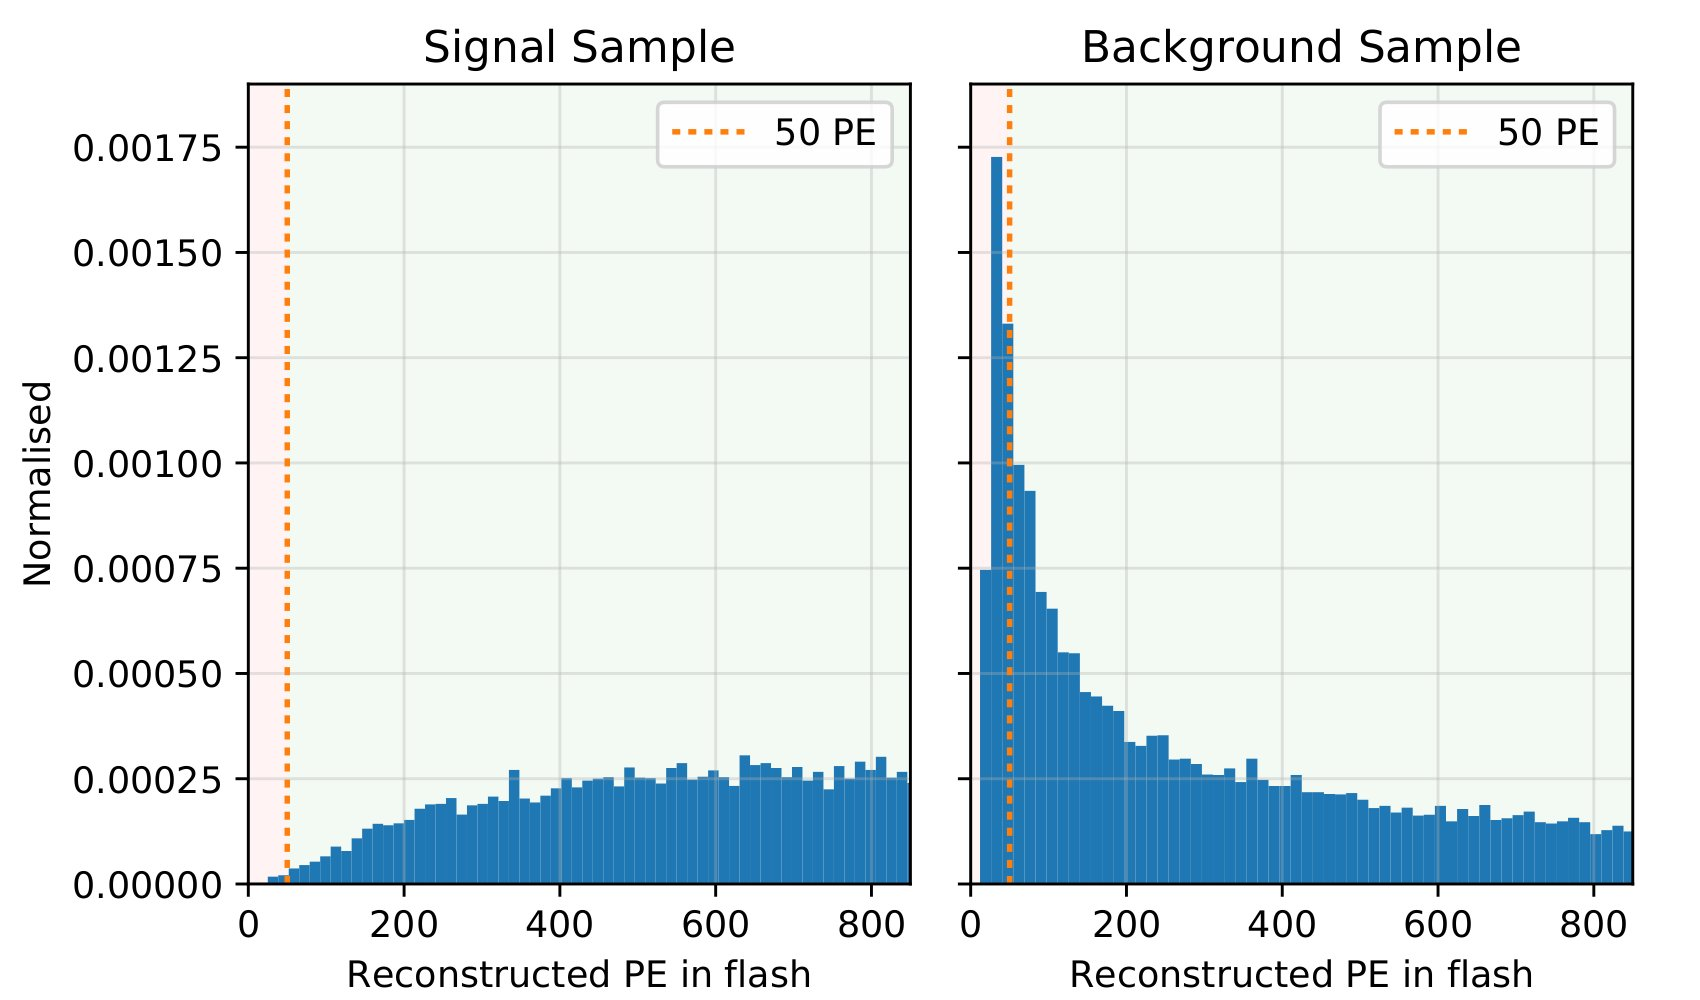
\includegraphics[width=0.85\textwidth]{figures/pe_cut.jpg} 
\caption{Reconstructed PE distribution for signal (left) and cosmic background (right) events.} 
\label{fig:pe_cut}
\end{figure}

These two cuts ensure that the event has a properly reconstructed flash. A flash object has a time and a PE count for each of the 32 PMTs. From this information, two coordinates $z\pm \sigma_z$ and $y\pm \sigma_y$ are calculated, where the positive $z$ axis corresponds to the beam direction and $y$ coordinate corresponds to the detector height. These two values can be compared with the centre of the deposited charge of the reconstructed neutrino candidate in the TPC. This comparison has the implicit assumption that the light will be emitted in the same relative fraction as the charge deposited by the particles in the final state. This is not completely correct since the amount of scintillation light produced per deposited energy unit depends on the particle. Nevertheless, the coarse resolution given by the PMT grid allows to use this approximation.

A cut of \SI{105}{\cm} is placed on the difference between the reconstructed flash position and the centre of the deposited charge on the $z$ axis. This cut keeps at least one neutrino candidate in 98.1\% of the signal events, and it removes all candidates in 20\% of the background events (Figure \ref{fig:z_cut}). 
Similar cuts are placed taking into account the width of the flash and its position on the $y$ axis. 

\begin{figure}[htbp]
\centering
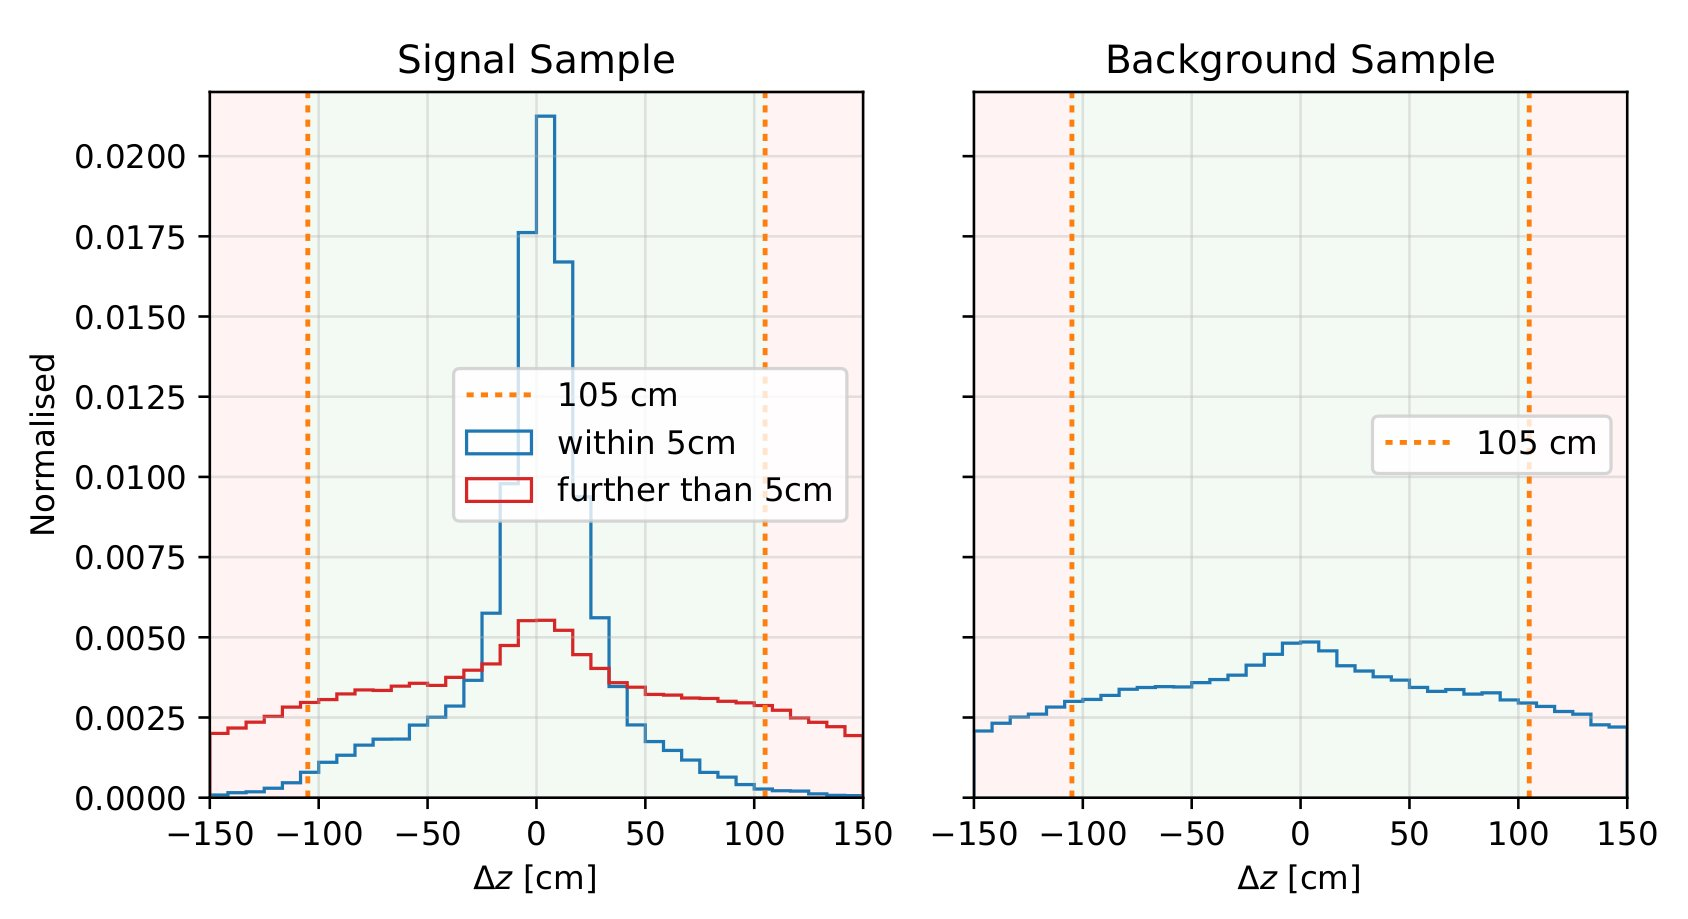
\includegraphics[width=0.85\textwidth]{figures/z_cut.jpg} 
\caption{Distribution of the distance between the reconstructed flash position and the centre of the deposited charge on the $z$ axis for signal (left) and cosmic background (right). The \emph{within 5 cm} and \emph{further than 5 cm} categories refers to the distance between the reconstructed neutrino vertex and the true neutrino vertex.} 
\label{fig:z_cut}
\end{figure}

The last rectangular cut exploits the fact that several neutrino candidates reconstructed by Pandora originate from remnants of cosmic activity which were not tagged by the cosmic-removal algorithms. Those neutrino candidates often consist in a small amount of fragmented charge, incompatible with the brightness of the flash. Placing a very conservative cut at 3.0 on the ratio between the charge in the collection plane associated to the neutrino candidate and the number of PEs reduces the signal events with a properly reconstructed flash by 1.7\%, while removing all candidates in 15.4\% of the background events (Figure \ref{fig:light_ratio}).

\begin{figure}[htbp]
\centering
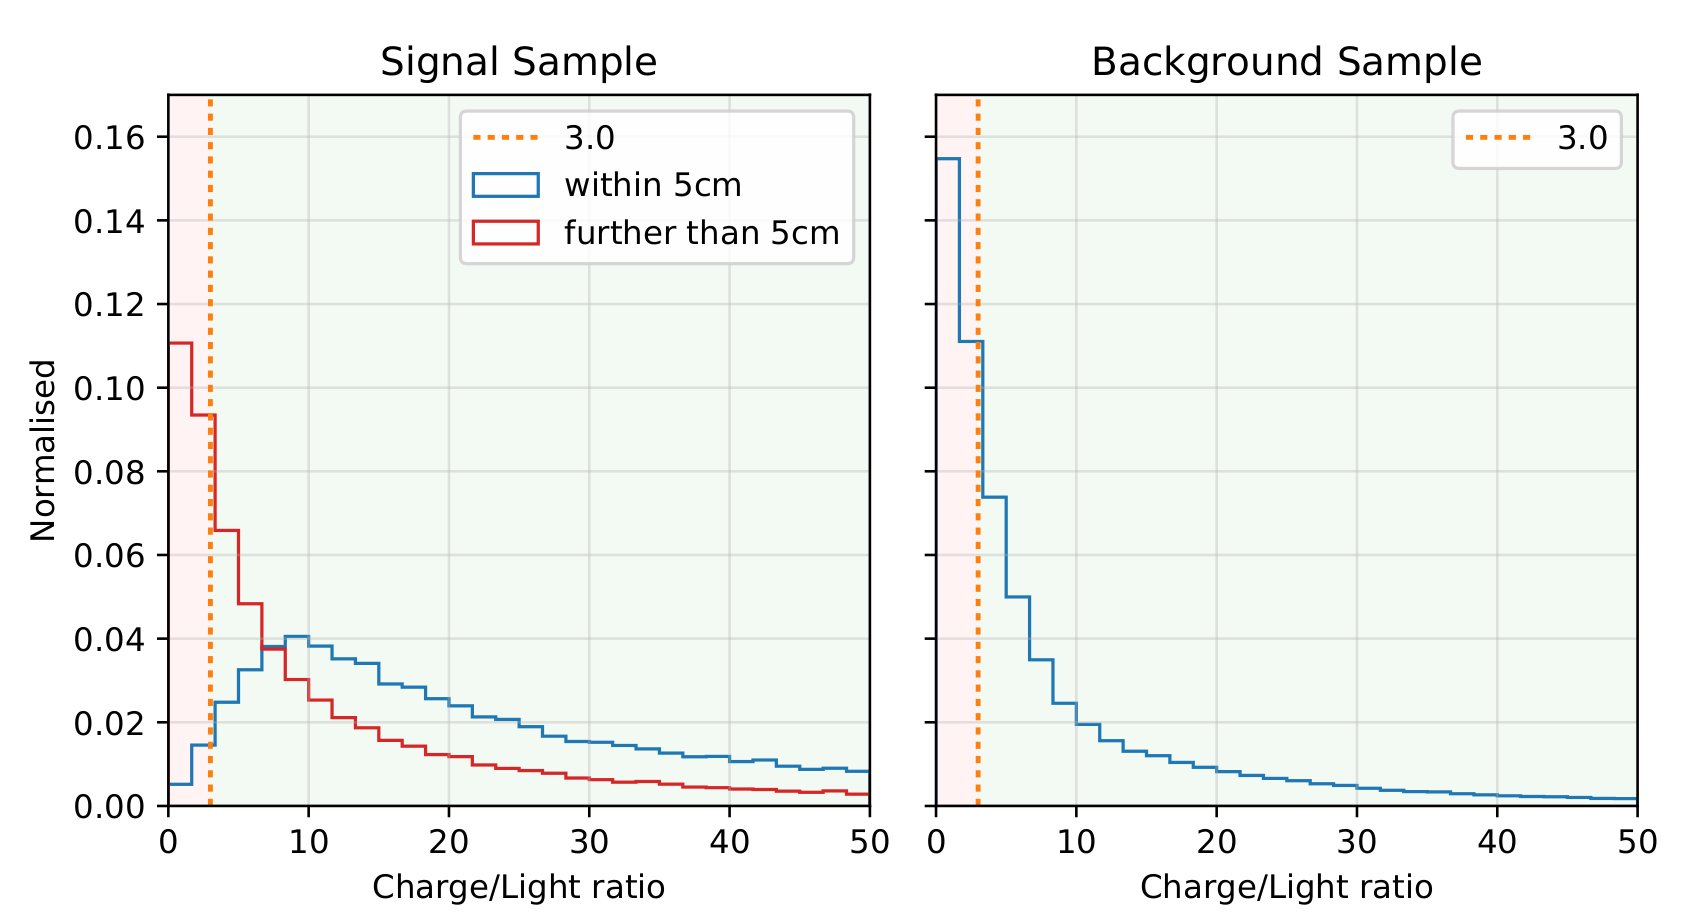
\includegraphics[width=0.85\textwidth]{figures/light_ratio.jpg} 
\caption{Distribution of the ratio between the charge in the collection plane associated to the neutrino candidate (in ADC counts) and the number of PEs collected by the PMTs. The \emph{within 5 cm} and \emph{further than 5 cm} categories refers to the distance between the reconstructed neutrino vertex and the true neutrino vertex.} 
\label{fig:light_ratio}
\end{figure}

After these rectangular cuts it is still possible to have more than one reconstructed neutrino candidate in the event. A more sophisticated flash-matching procedure allows to choose the one that best matches the collected light:
\begin{enumerate}
\item for every neutrino candidate, a spatial distribution of deposited charge is measured;
\item the spatial distribution of the deposited charge is translated into an estimation of the emitted scintillation light. These scintillation photons are then propagated towards the PMTs to construct a flash hypothesis using only TPC information;
\item the flash-matching algorithm compares the reconstructed flash object as seen by the PMTs with the hypothetical flash for every reconstructed neutrino candidate and picks the best-matching candidate. This selection is achieved through a binned likelihood of the PMT spectrum.
\end{enumerate}


An example of this procedure for a Monte Carlo generated $\nu_e$ event with 4 neutrino candidates is given in Figure~\ref{fig:flashmatch}.

\begin{figure}[htbp]
\centering
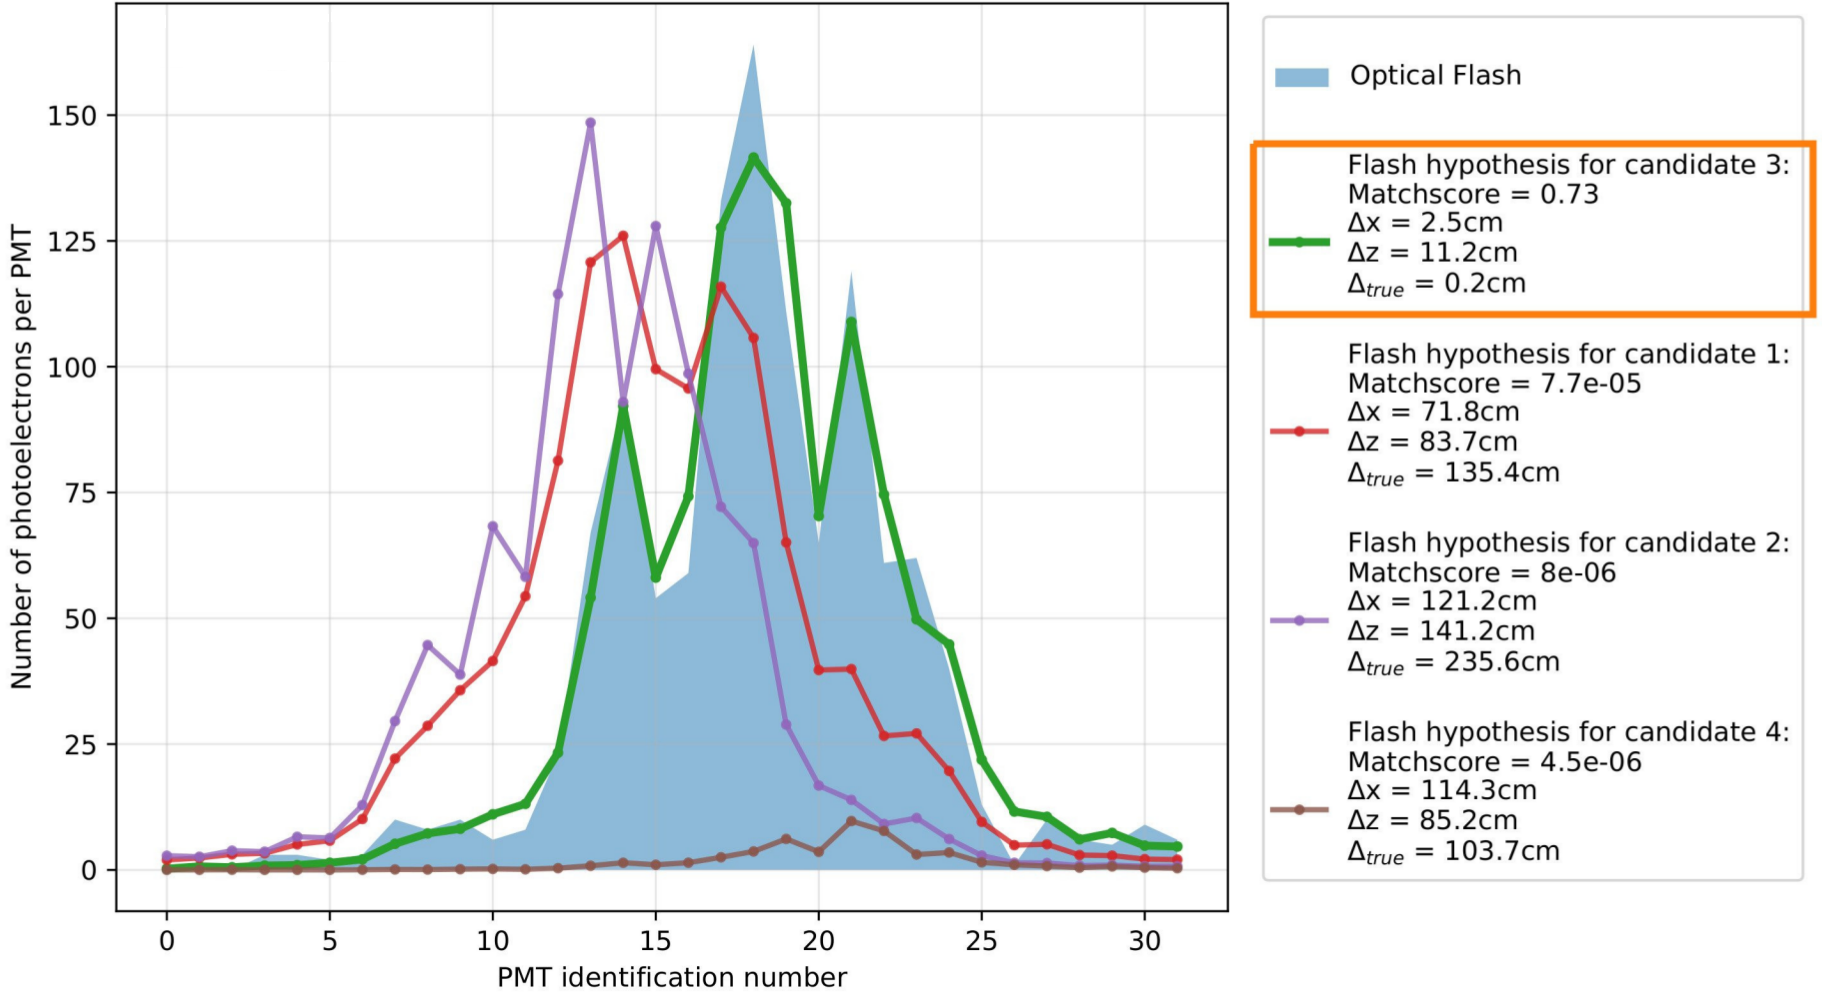
\includegraphics[width=0.85\textwidth]{figures/flashmatch.png} 
\caption{An example of flash-matching. The event has 4 neutrino candidates and we make a flash hypothesis for each one, shown in red, purple, green, and brown. The observed flash corresponds to the filled blue area. A minimum binned likelihood is calculated, varying the $x$ position of the interaction. The match score is the inverse of the likelihood. The candidate with the highest match score is chosen as neutrino interaction candidate (the green one in this case).} 
\label{fig:flashmatch}
\end{figure}

\subsection{Topological pre-selection} \label{sec:topological_pre_selection}
A perfect reconstruction of a $\nu_{e}$ CC0$\pi$-Np event in a LArTPC will produce as many reconstructed tracks as the number of protons above the detection threshold in the final state and a single reconstructed shower (the electron), sharing a common vertex. However, mis-reconstruction and mis-classification issues can significantly lower the selection efficiency. The current status of the event reconstruction, which depends on the properties of the event (e.g. the number of hits \cite{Acciarri:2017hat}), affects the efficiency of selecting these events. For example, the presence of dead or unresponsive wires can affect the reconstruction by causing the splitting of an ionisation track or an electromagnetic shower into two distinct reconstructed objects. Also, the selection currently implemented relies on the classification of the reconstructed objects as track-like or shower-like, a separation that contains an inherent inefficiency, especially when the number of reconstructed hits is low.

In order to maximise our efficiency we currently require (1) \emph{at least} one track and \emph{at least} one shower sharing a common vertex, or (2) \emph{at least} two showers sharing a common vertex, to account for proton mis-classification as a shower-like object. This is because it is much more common to have protons classified as showers than electrons classified as tracks. For these cases we measure the $\chi^2$ score of the $dE/dx$ vs. residual range profile of the reconstructed objects in the proton hypothesis, as described in Section \ref{sec:proton_id}. The object with the lowest proton $\chi^2$ score is classified as a track, while the other ones remain classified as showers.

\subsection{Minimum reconstruction quality requirements}\label{sec:precuts}
A minimal set of cuts is applied to the selected events, in order to ensure that they are well reconstructed.
First, to avoid border effects, the reconstructed neutrino vertex, the start point of the reconstructed showers and the start and end points of the reconstructed tracks are required to lie within a fiducial volume. Our fiducial volume cut is 10~cm from each side on the $x$ axis, 15~cm from each side on the $y$ axis, and 10~cm (40~cm) from the upstream (downstream) side on the $z$ axis (Figure \ref{fig:fidvol}). The fiducial volume corresponds to 76.4\% of the total TPC volume. 

\begin{figure}
\centering
  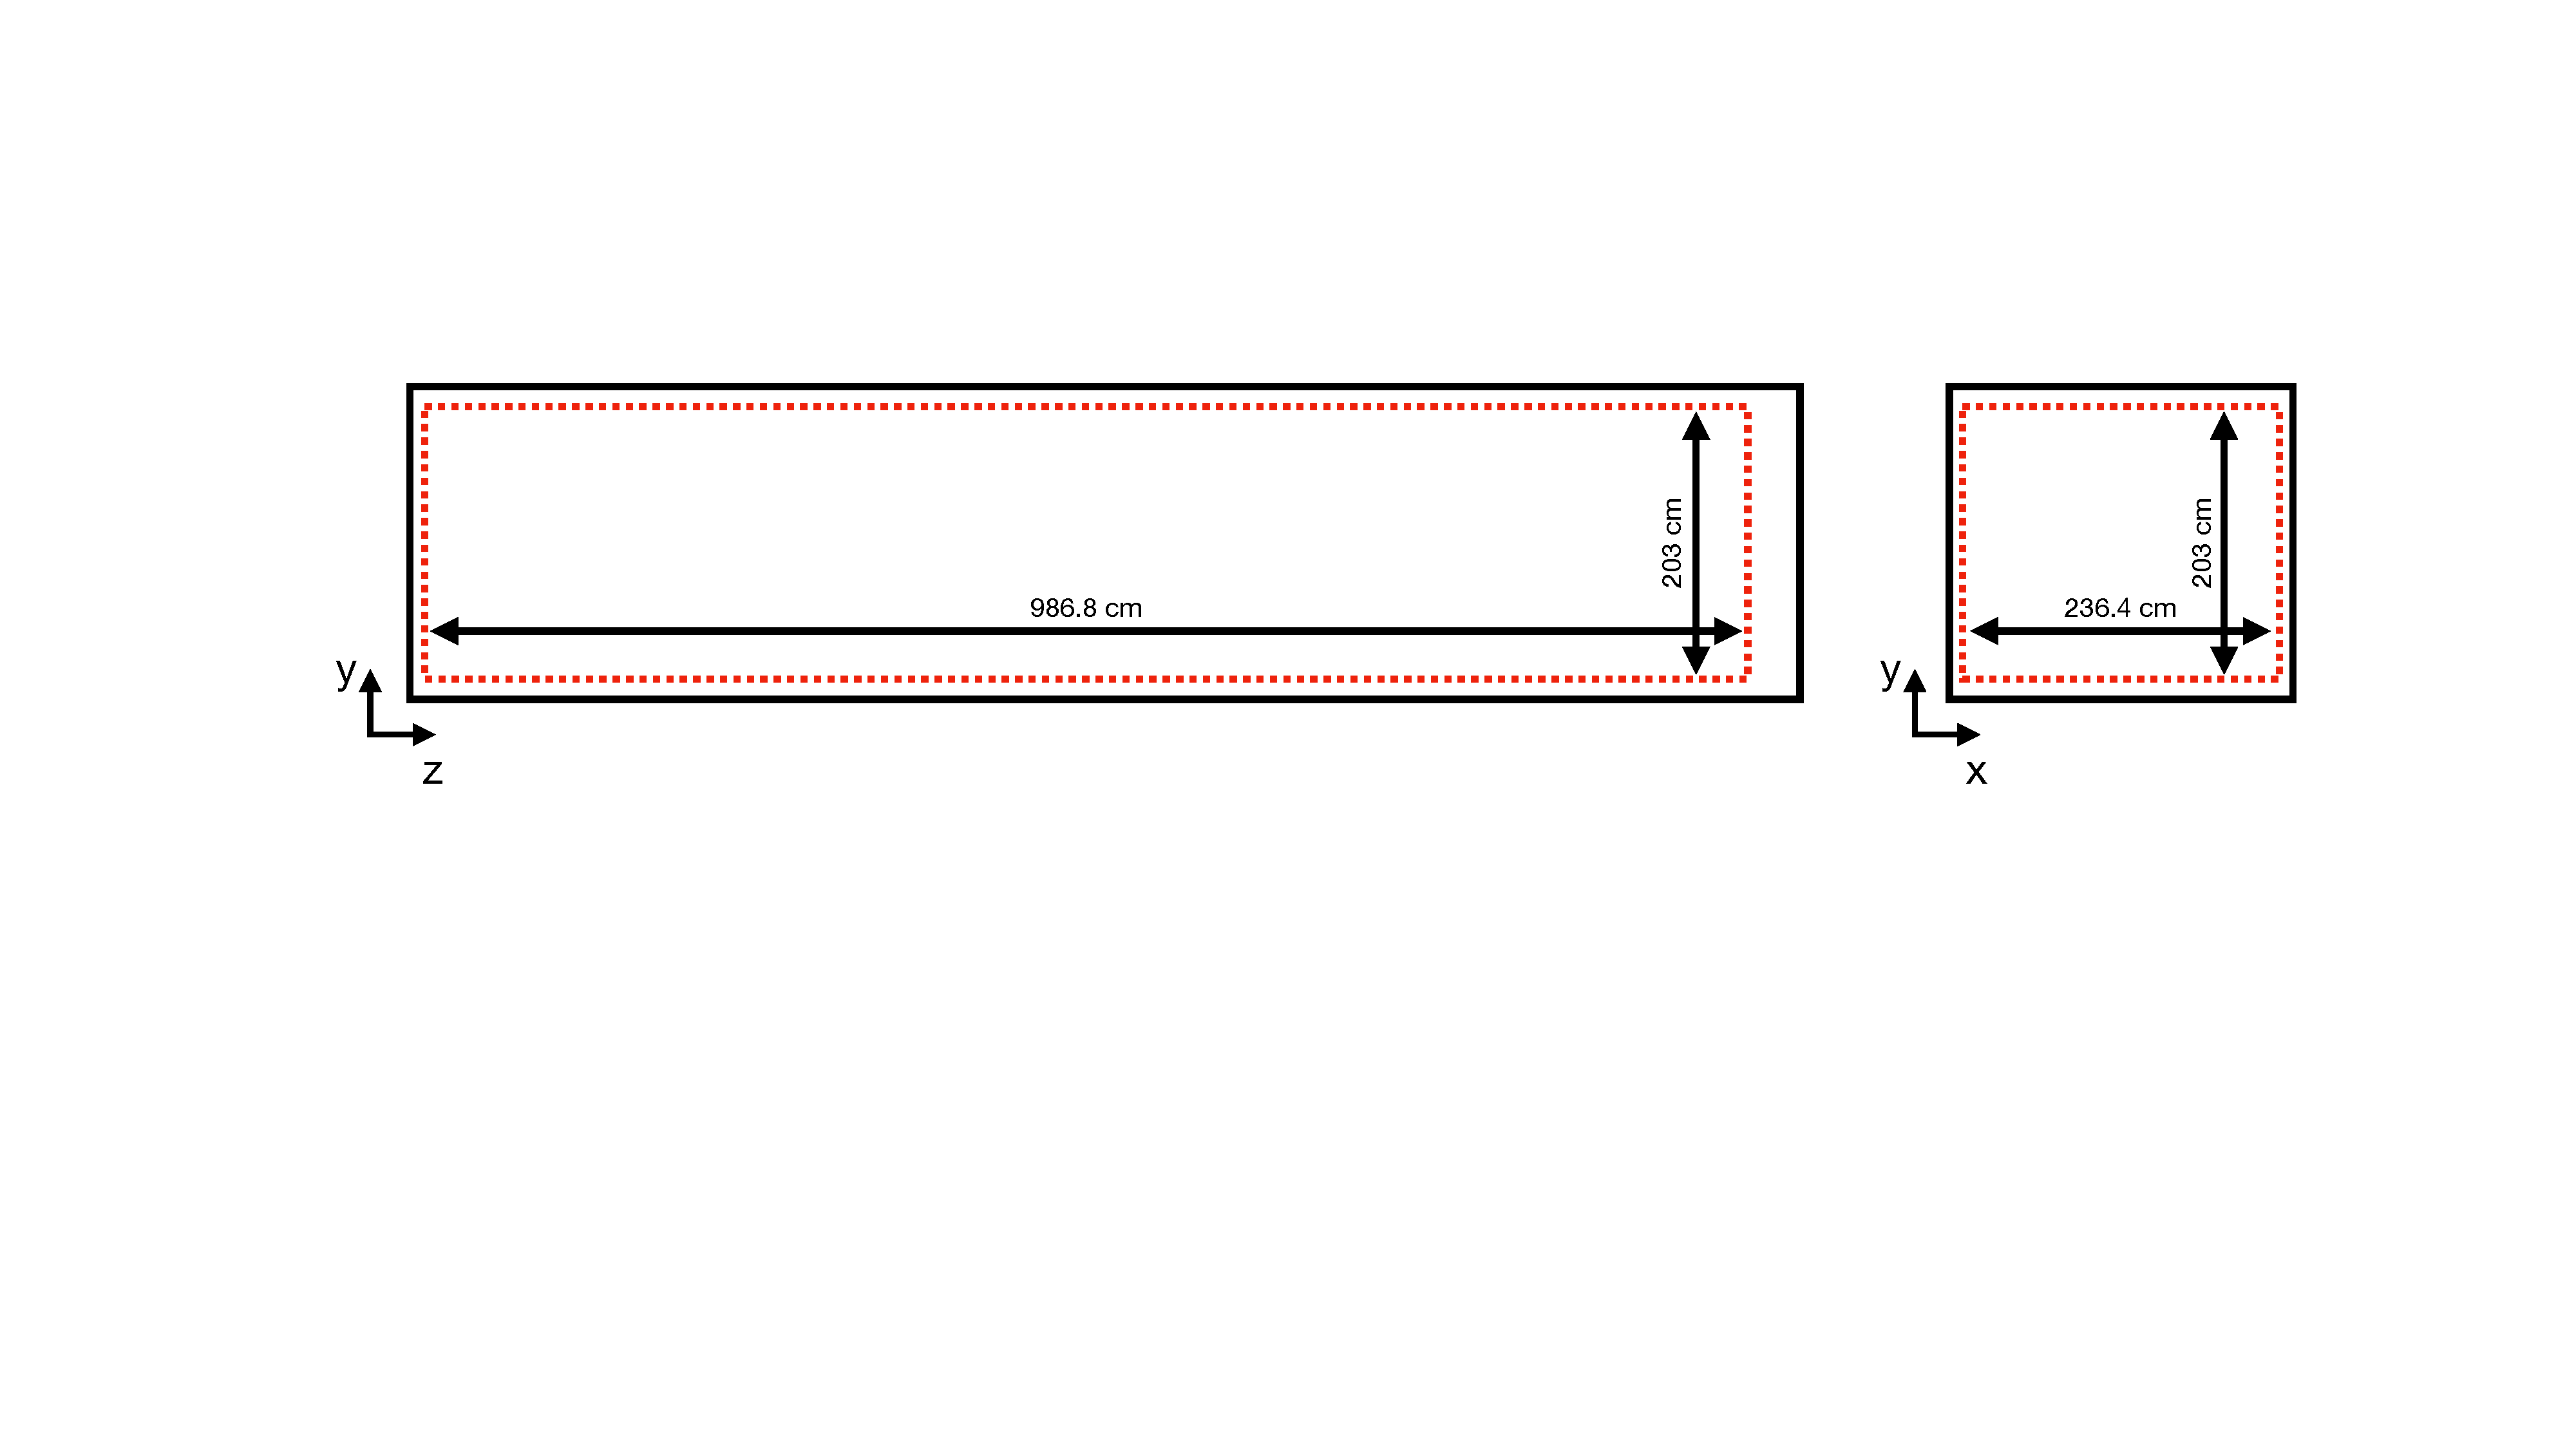
\includegraphics[width=0.95\linewidth]{figures/fidvol.pdf}
  \caption{Schematic of the fiducial volume used in this analysis. The solid line corresponds to the TPC borders and the dashed red line corresponds to the fiducial volume borders.}
  \label{fig:fidvol}
\end{figure}

Since electromagnetic showers develop mainly in the forward direction with respect to the beam, the asymmetric cut on the $z$ axis (which corresponds to the beam direction) helps to reject non-fully contained events which begin too close to the downstream end of the TPC.
We also require, for each event, (1) at least 5 hits in the three planes associated to shower-like objects, (2) at least 5 hits in the three planes associated to track-like objects, and (3) at least one hit in every plane.


\subsection{Selection efficiency and purity}\label{sec:eff}
The selection efficiency of our algorithm is obtained by calculating the fraction of events selected in the $\nu_{e}$ CC$0\pi$-Np + cosmic Monte Carlo sample, where the true neutrino vertex, the start and end points of the protons, and the start point of the electron are fully contained in the fiducial volume.

In order to understand what energy thresholds are appropriate for reconstruction in the TPC, dedicated studies have been performed on proton tracks and electron showers, using the $\nu_{e}$ CC$0\pi$-Np + cosmic Monte Carlo sample, shown in Figure \ref{fig:thresholds}. We have found that we have no efficiency for reconstructing and classifying protons {with a kinetic energy} below 40~MeV and electrons{, photons, and charged pions} {with a kinetic energy} below 30~MeV following these optical, topological, and minimum quality pre-selections. Therefore, these energy thresholds are applied to the simulations to allow a fair comparison with the reconstructed particles. 

\begin{figure}
\centering
  \begin{subfigure}{0.48\textwidth}
    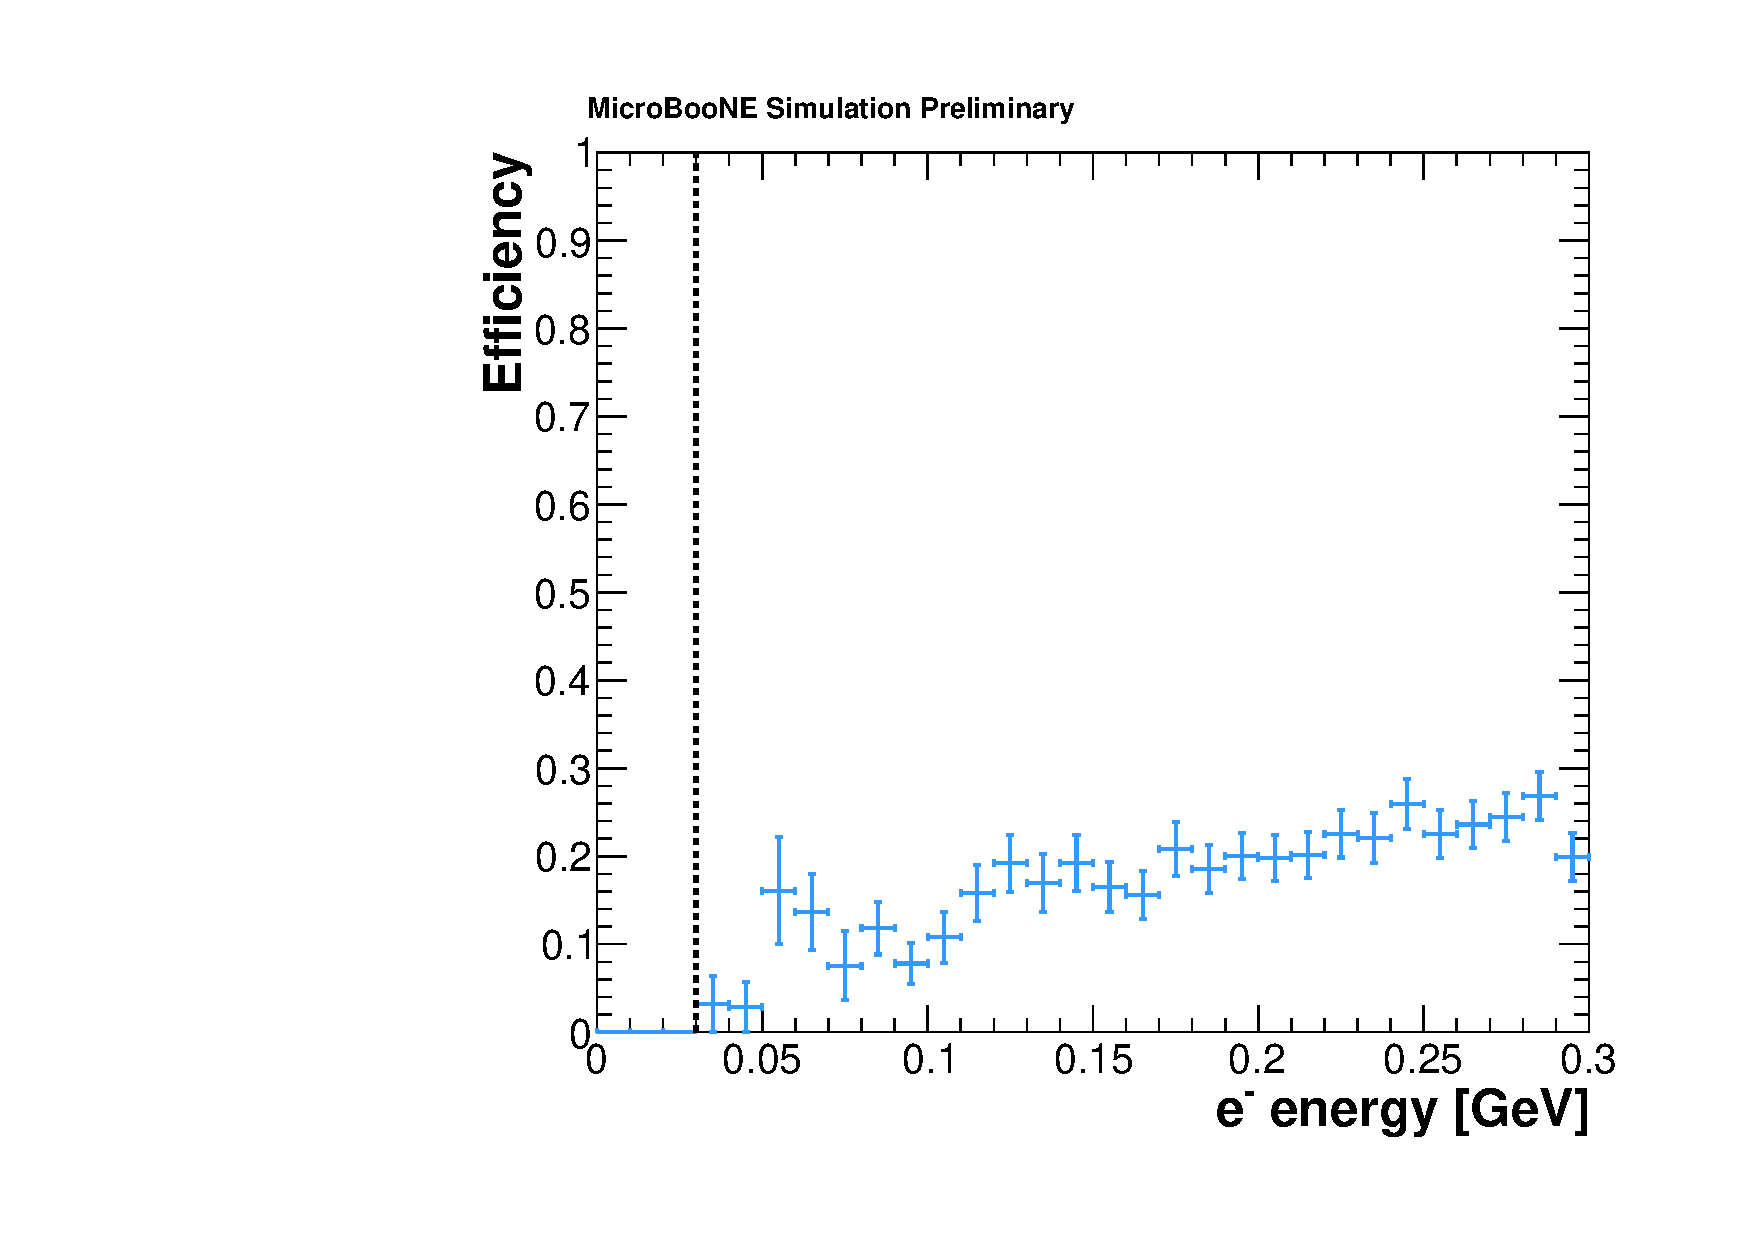
\includegraphics[width=\linewidth]{figures/e_efficiency.pdf}
    \caption{Electron efficiency.} 
  \end{subfigure}
    \begin{subfigure}{0.48\textwidth}
    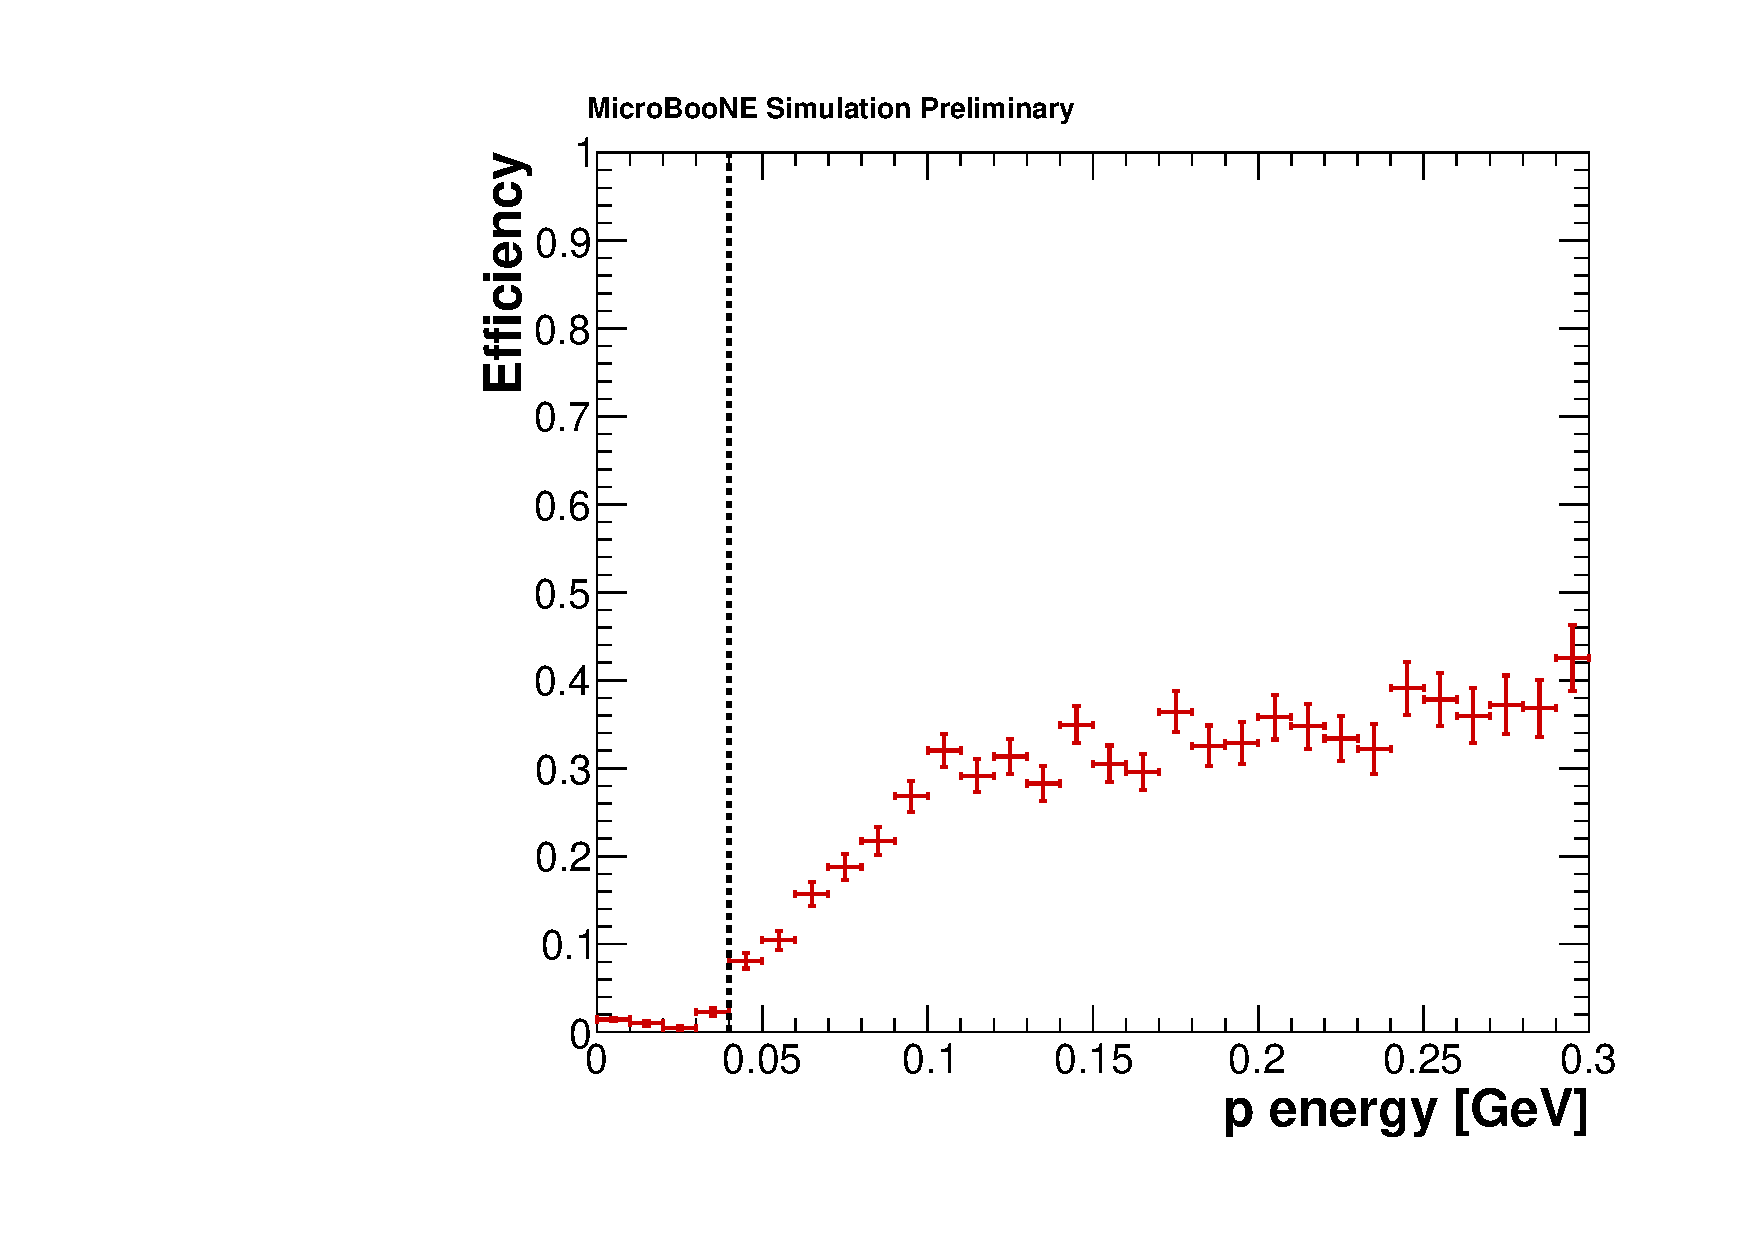
\includegraphics[width=\linewidth]{figures/p_efficiency.pdf}
    \caption{Proton efficiency.} 
  \end{subfigure}
  \caption{$\nu_{e}$ CC$0\pi$-Np selection efficiency on single particles as a function of the true electron (left) and proton (right) kinetic energy. The dashed lines correspond to the threshold applied at truth level.}
  \label{fig:thresholds}
\end{figure}


Our overall $\nu_{e}$ CC$0\pi$-Np selection efficiency $\epsilon$ is defined as:
\begin{equation}
\epsilon = \frac{\mathrm{N.~of~selected~}\nu_{e}\mathrm{~CC0}\pi\mathrm{{\text -}Np~events}}{\mathrm{N.~of~generated~}\nu_{e}\mathrm{~CC0}\pi\mathrm{{\text -}Np~events}},
\end{equation}
where each selected event must pass the optical selection, satisfy the topology and minimum quality requirements, and not being vetoed by the independent CC $\nu_{\mu}$ selection module. %Figure \ref{fig:thresholds} shows the selection efficiency as a function of the electron and the proton kinetic energies. 



The true neutrino energy spectrum of the simulated $\nu_{e}$ CC$0\pi$-Np events in the $[0,3]$~GeV range is shown in Figure \ref{fig:true_energy}.

\begin{figure}
\centering
  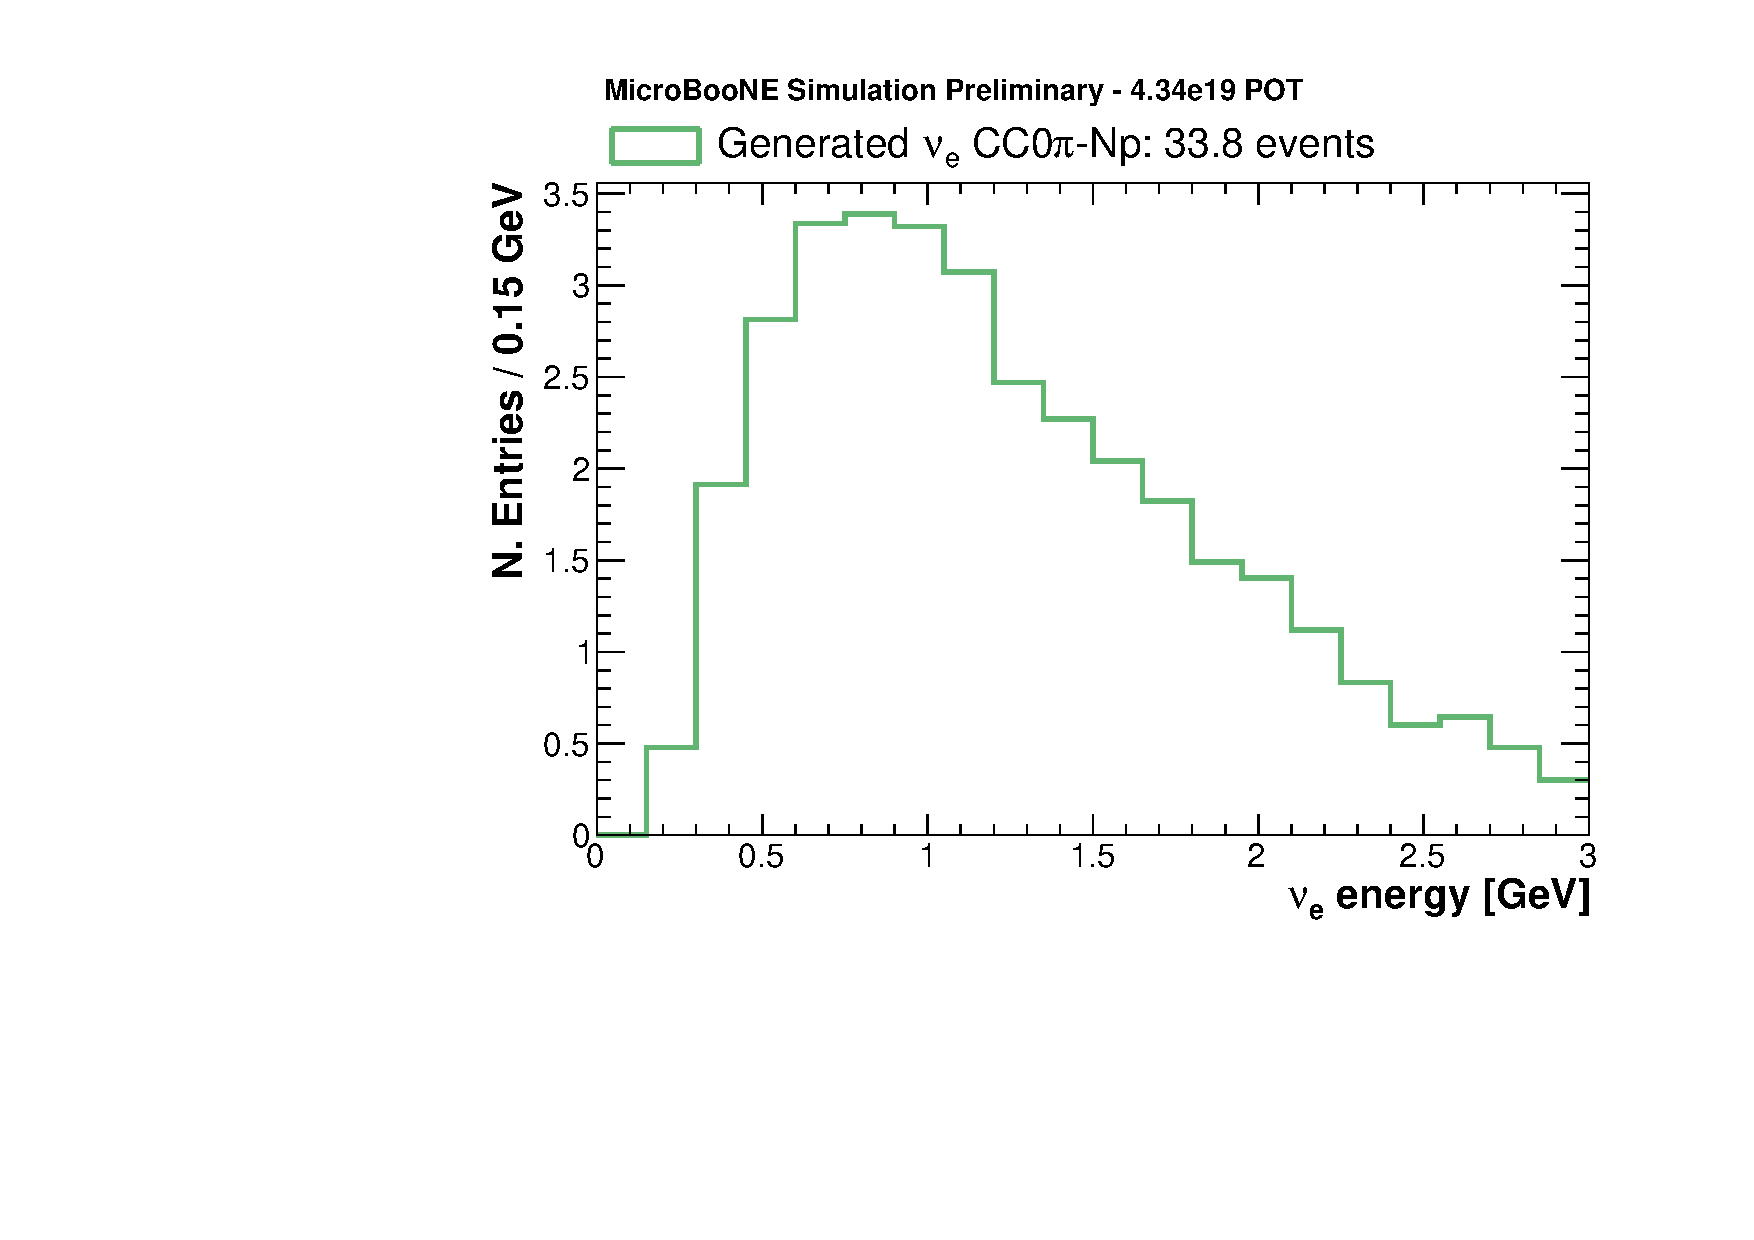
\includegraphics[width=0.8\linewidth]{figures/tot.pdf}
  \caption{Simulated $\nu_{e}$ CC$0\pi$-Np true neutrino energy spectrum in the 0-3~GeV range. Each true proton (true electron) in the final state is required to have a kinetic energy larger than 40~MeV (30~MeV).}
  \label{fig:true_energy}
\end{figure}

Figure \ref{fig:effpurity} shows the efficiency as a function of the true neutrino energy.
%The energy reconstruction procedure is described in section \ref{sec:energyreco}.
The systematic uncertainties related to the cross-section and the neutrino beam flux, described in Chapter \ref{sec:systematics}, are also included. The inner error bars represent the Monte Carlo statistical uncertainty, while the outer error bars are obtained summing in quadrature the statistical and the systematic uncertainties. The statistical uncertainty $\delta\epsilon$ corresponds to the binomial error, since the application of a selection can be considered a binomial process \cite{Paterno:2004cb}:
\begin{equation}
    \delta\epsilon = \frac{1}{N}\sqrt{k(1-k/N)},
\end{equation}
where $k$ is the number of selected events and $N$ is the total number of events.

As expected, the efficiency increases with the neutrino energy, since high-energy neutrino interactions correspond in general to a larger number of hits in the TPC and the Pandora framework reconstruction performances increase with the number of reconstructed hits \cite{Acciarri:2017hat}. 

%A description of future improvements, which will allow us to increase the selection efficiency, is included in Section \ref{sec:future}.

% \todo{Add efficiency plots over a larger energy region for protons and electrons.}

\begin{figure}
\centering
%   \begin{subfigure}{0.48\textwidth}
    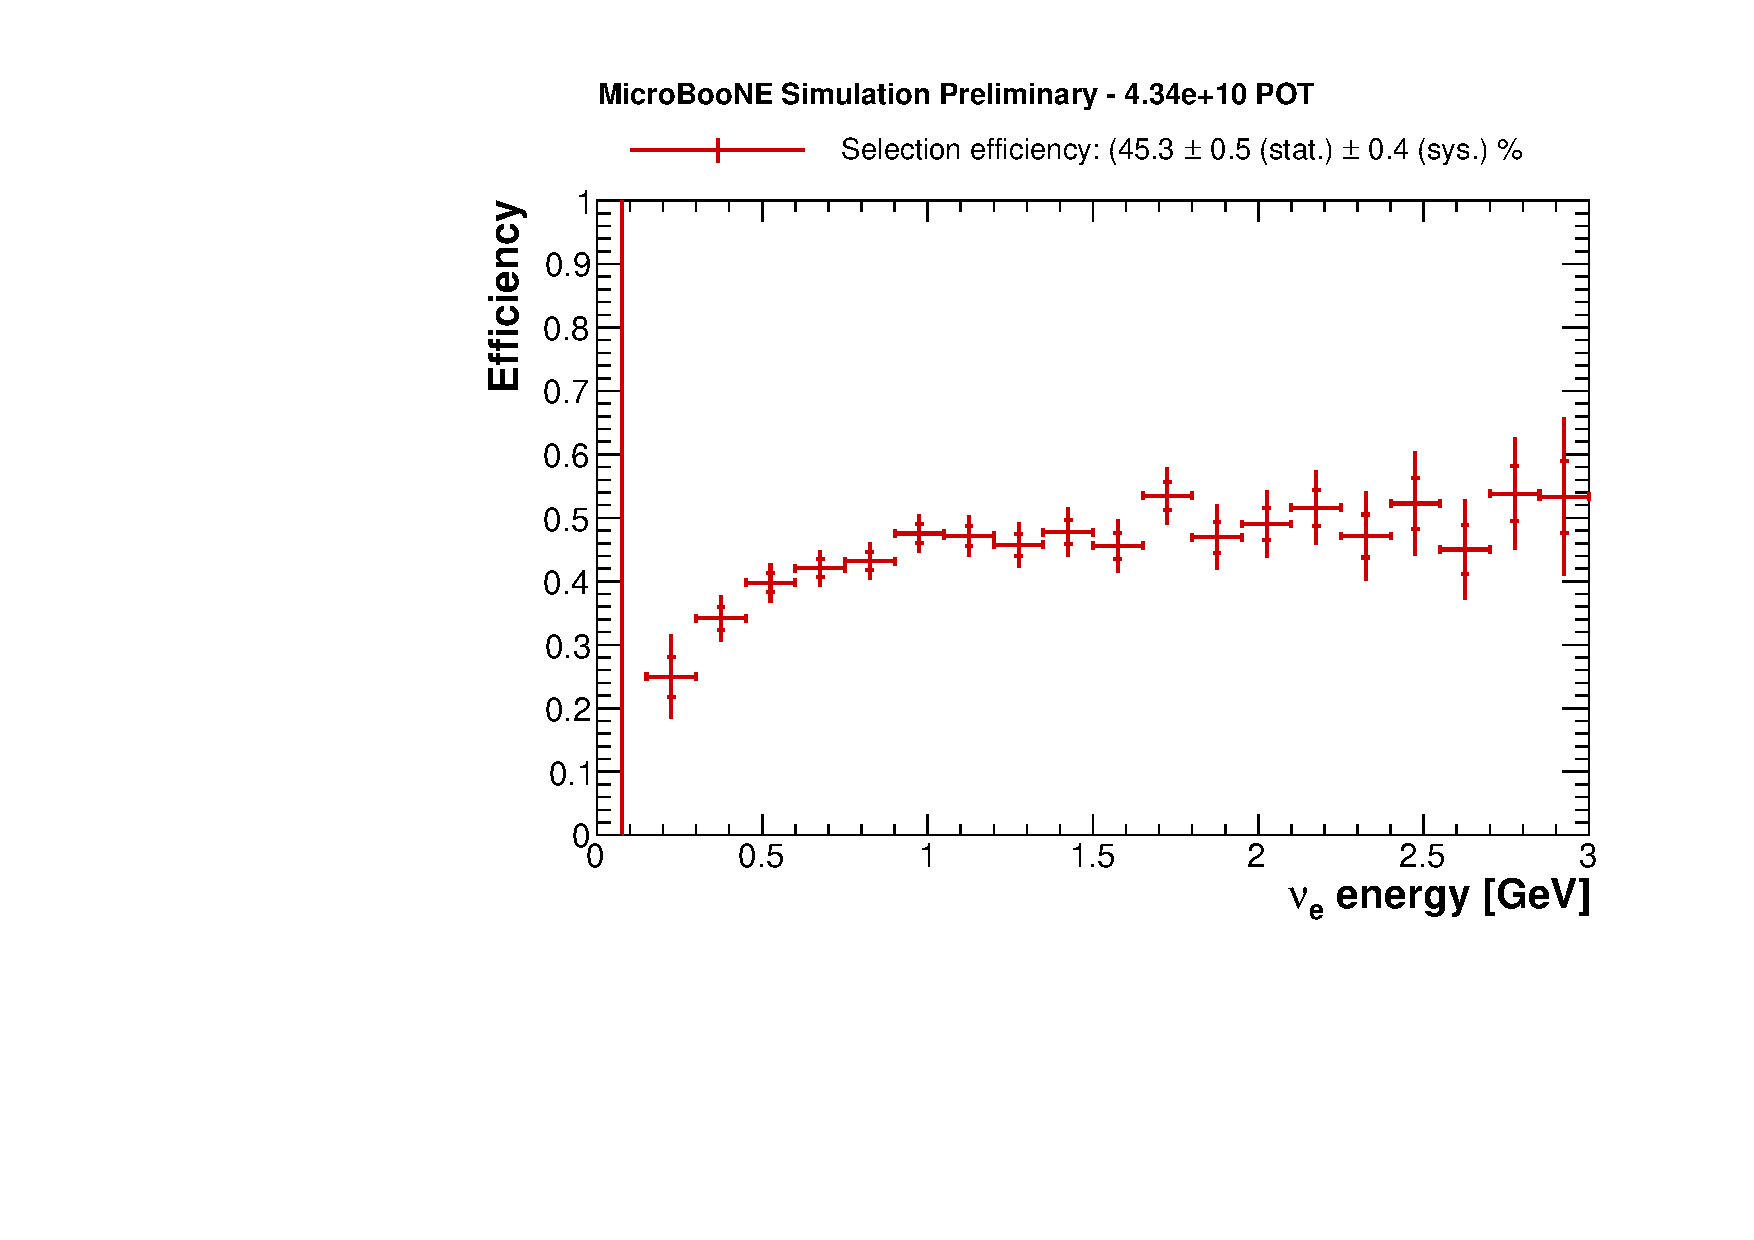
\includegraphics[width=0.8\linewidth]{figures/eff.pdf}
%     \caption{Efficiency.} 
%   \end{subfigure}
%     \begin{subfigure}{0.48\textwidth}
%     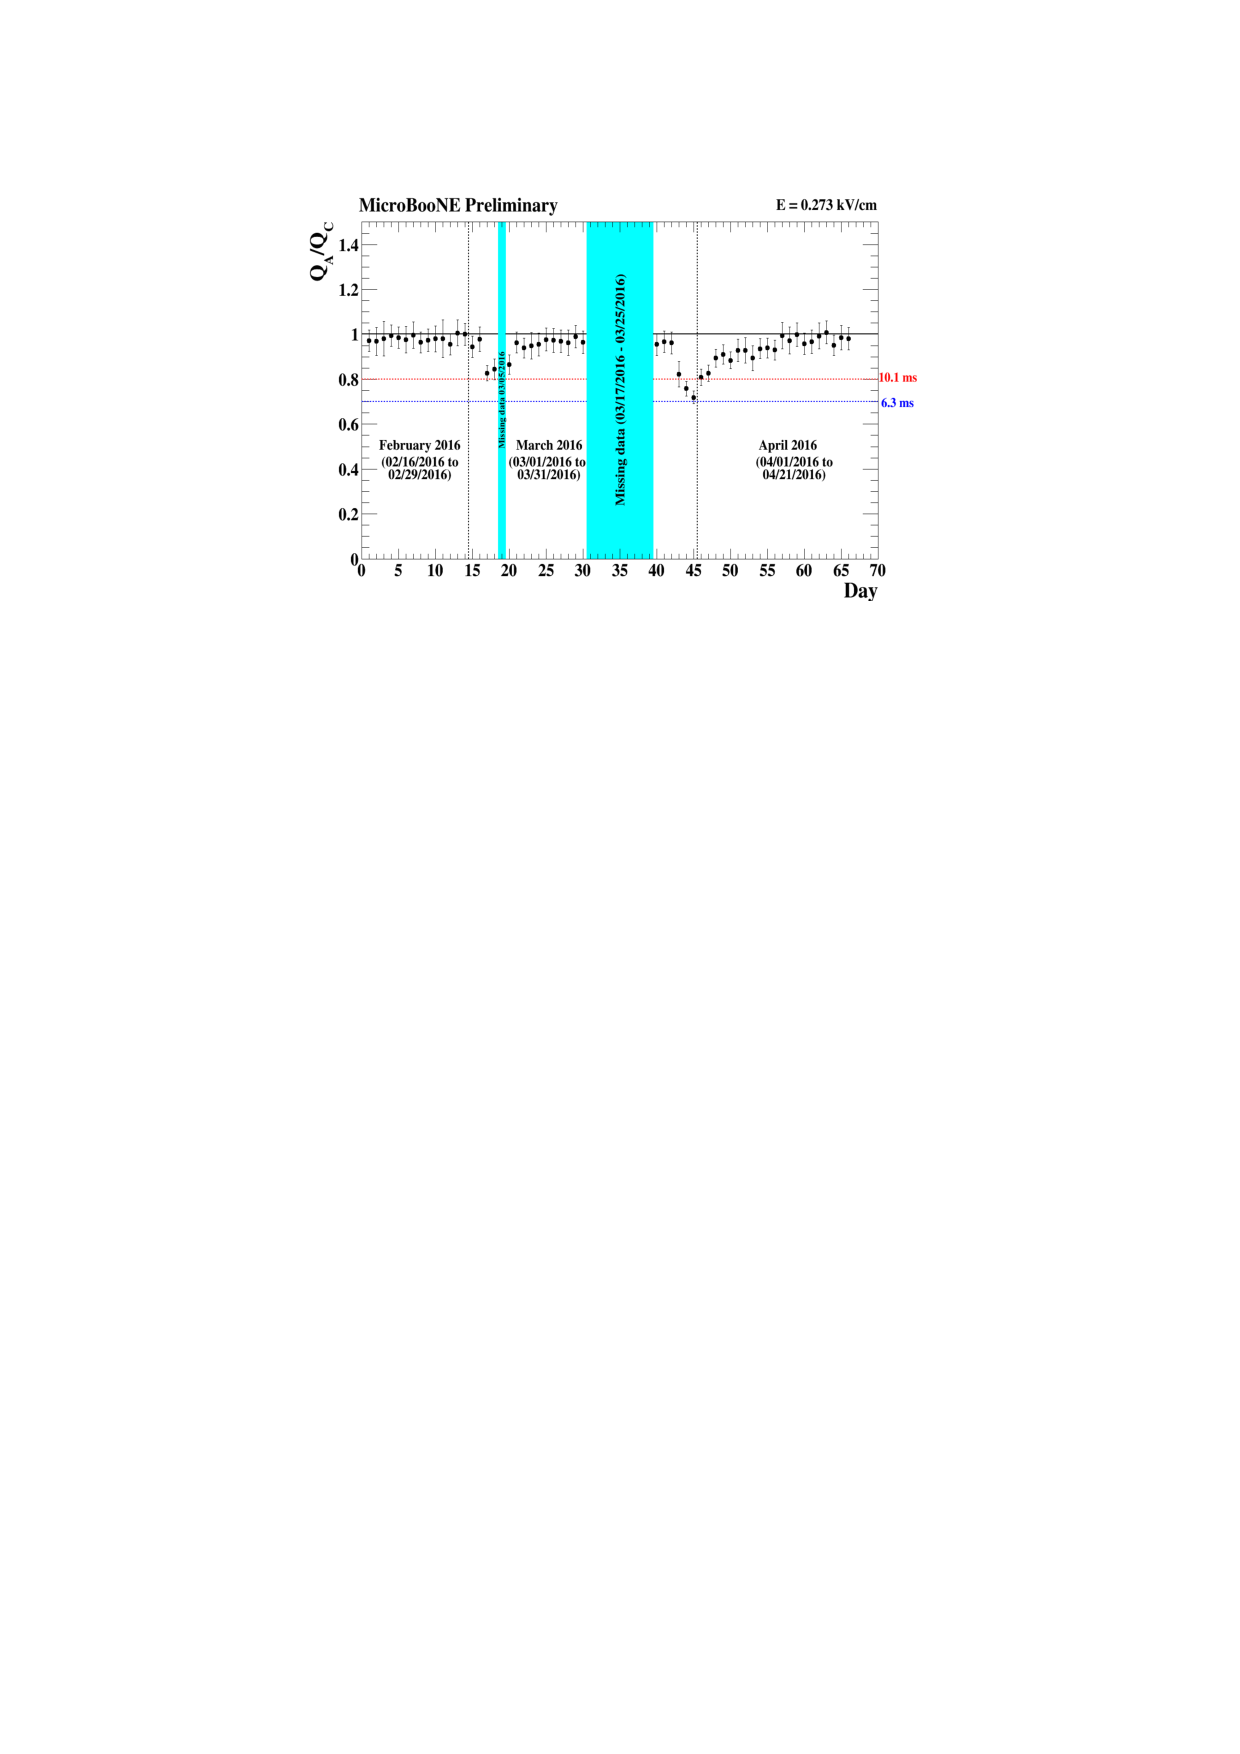
\includegraphics[width=\linewidth]{figures/purity.pdf}
%     \caption{Purity.} 
%   \end{subfigure}
  \caption{$\nu_{e}$ CC$0\pi$-Np selection efficiency as a function of the true $\nu_{e}$ energy. Each true proton (true electron) in the final state is required to have a kinetic energy larger than 40~MeV (30~MeV). The inner error bars represent the Monte Carlo statistical uncertainty, while the outer error bars are obtained summing in quadrature the statistical and the systematic uncertainties.}
  \label{fig:effpurity}
\end{figure}

\subsubsection{Inefficiencies breakdown}\label{sec:ineff}
Our current selection algorithm can fail for several reasons: in particular, we could have problems in the classification, such as an electron classified as a track-like object, or particles not reconstructed at all. We identified eight main causes for our selection inefficiency, whose contributions have been estimated with the same simulated sample described in Section \ref{sec:eff}. The different contributions can be visualised in Figure \ref{fig:ineff} and are described below.
\begin{description}

\item[Quality cuts (8.5\%).] The selected neutrino candidate does not satisfy our minimum quality requirements, such as the number of shower hits and the number of track hits (Section \ref{sec:precuts}).
\item[CC $\nu_{\mu}$ selected (4.3\%).] The event is tagged as a CC $\nu_{\mu}$ candidate by an independent selection module, described in \cite{ubxsec}. 
\item[Not contained (10.1\%).] One of the reconstructed tracks or the starting point of one of the reconstructed showers is not contained in the fiducial volume. As expected, this fraction increases with the neutrino energy.
\item[Cosmic selected (7.9\%).] The selected neutrino candidate has one or more reconstructed objects of cosmic origin.
\item[1 shower (3.5\%).] The selected neutrino candidate has only one associated reconstructed shower and no track object. 
\item[No showers (13.7\%).]  The selected neutrino candidate has only reconstructed track(s) associated. This is the largest contribution to the inefficiency, especially at low energies, since low-energy electrons are very challenging to reconstruct and classify as showers.
\item[No flash (5.7\%).]  The flash collected by the optical system does not satisfy our requirements, such as the minimum number of PE, location of the flash and flash hypothesis (Section \ref{sec:optical_pre_cuts}).
\item[No data products (0.7\%).] The Pandora pattern recognition did not identify any neutrion candidate.
\end{description}

Figure \ref{fig:ineff} shows a stacked histogram of the true neutrino energy for the $\nu_e$~CC0$\pi$-Np generated events, divided into the categories described above. The events without a reconstructed shower are the dominant inefficiency at low energy. Low-energy showers correspond in general to a smaller number of reconstructed hits, which makes the pattern recognition more challenging \cite{Acciarri:2017hat}. The fraction of events where at least one reconstructed object is not contained in the detector (\emph{not contained} in the legend) increases with the energy. This is expected, since the probability to have large electromagnetic showers split in two or more object increases, and these objects can have a vertex reconstructed outside the fiducial volume. The \emph{passed} category (filled grey histogram) corresponds to the efficiency plot shown in Figure \ref{fig:effpurity}.

\begin{figure}
\centering
  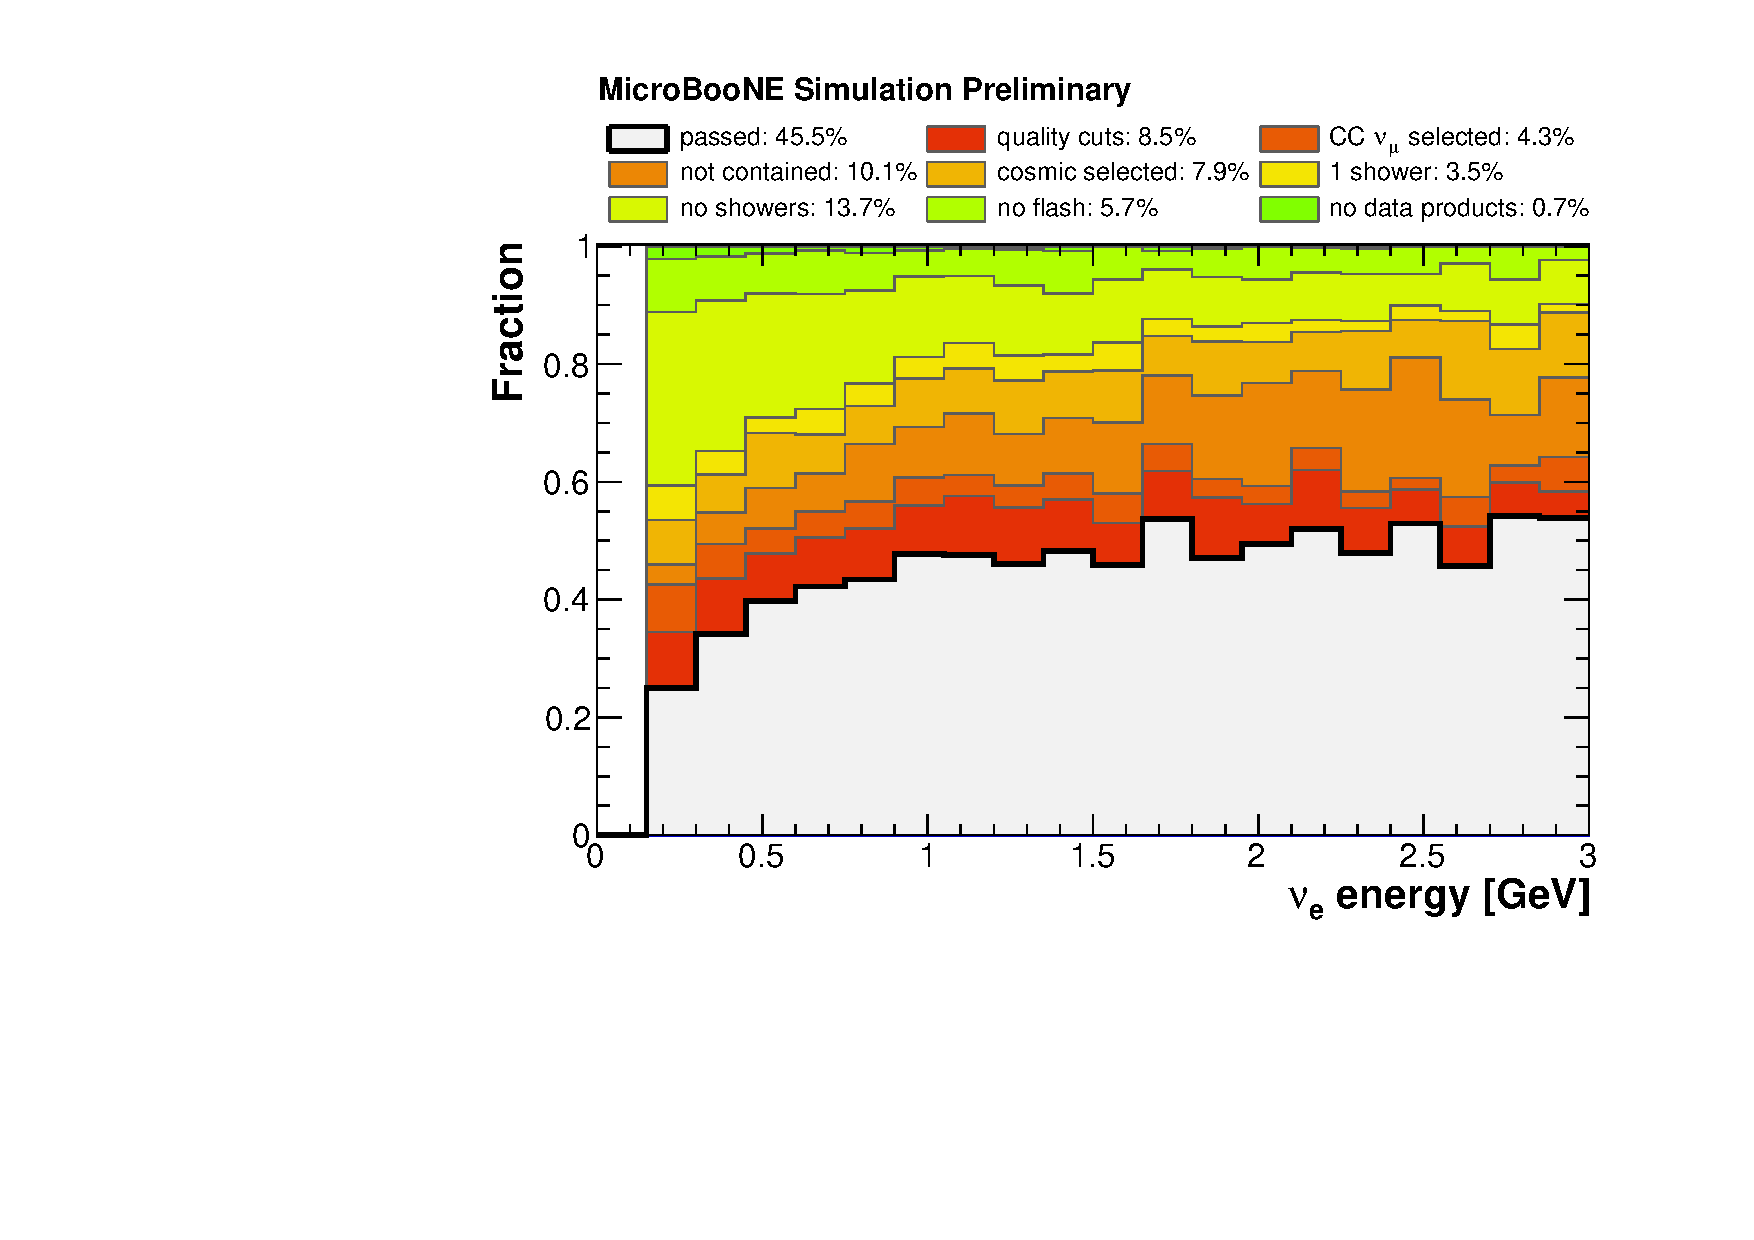
\includegraphics[width=0.8\linewidth]{figures/ineff_ene.pdf}
  \caption{Stacked histogram of generated events as a function of the true neutrino energy, categorised into correctly identified signal events in grey {(\emph{passed})} and different reconstruction or identification failure modes in colour.}
  \label{fig:ineff}
\end{figure}

For more detailed information, the selection outcomes as a function of the lepton true angular variables $\theta$ and $\phi$ are shown in Figure \ref{fig:ineff_angles}. The efficiency is mostly constant as a function of the azimuthal angle $\phi$, while the fraction of events without reconstructed showers increases as a function of the $\theta$ angle. This is because backwards-going electrons are more difficult to reconstruct, since they often have lower energy, and the pattern recognition tends to group the electron hits together with the forward-going proton track.

\begin{figure}
\centering
  \begin{subfigure}{0.48\textwidth}
    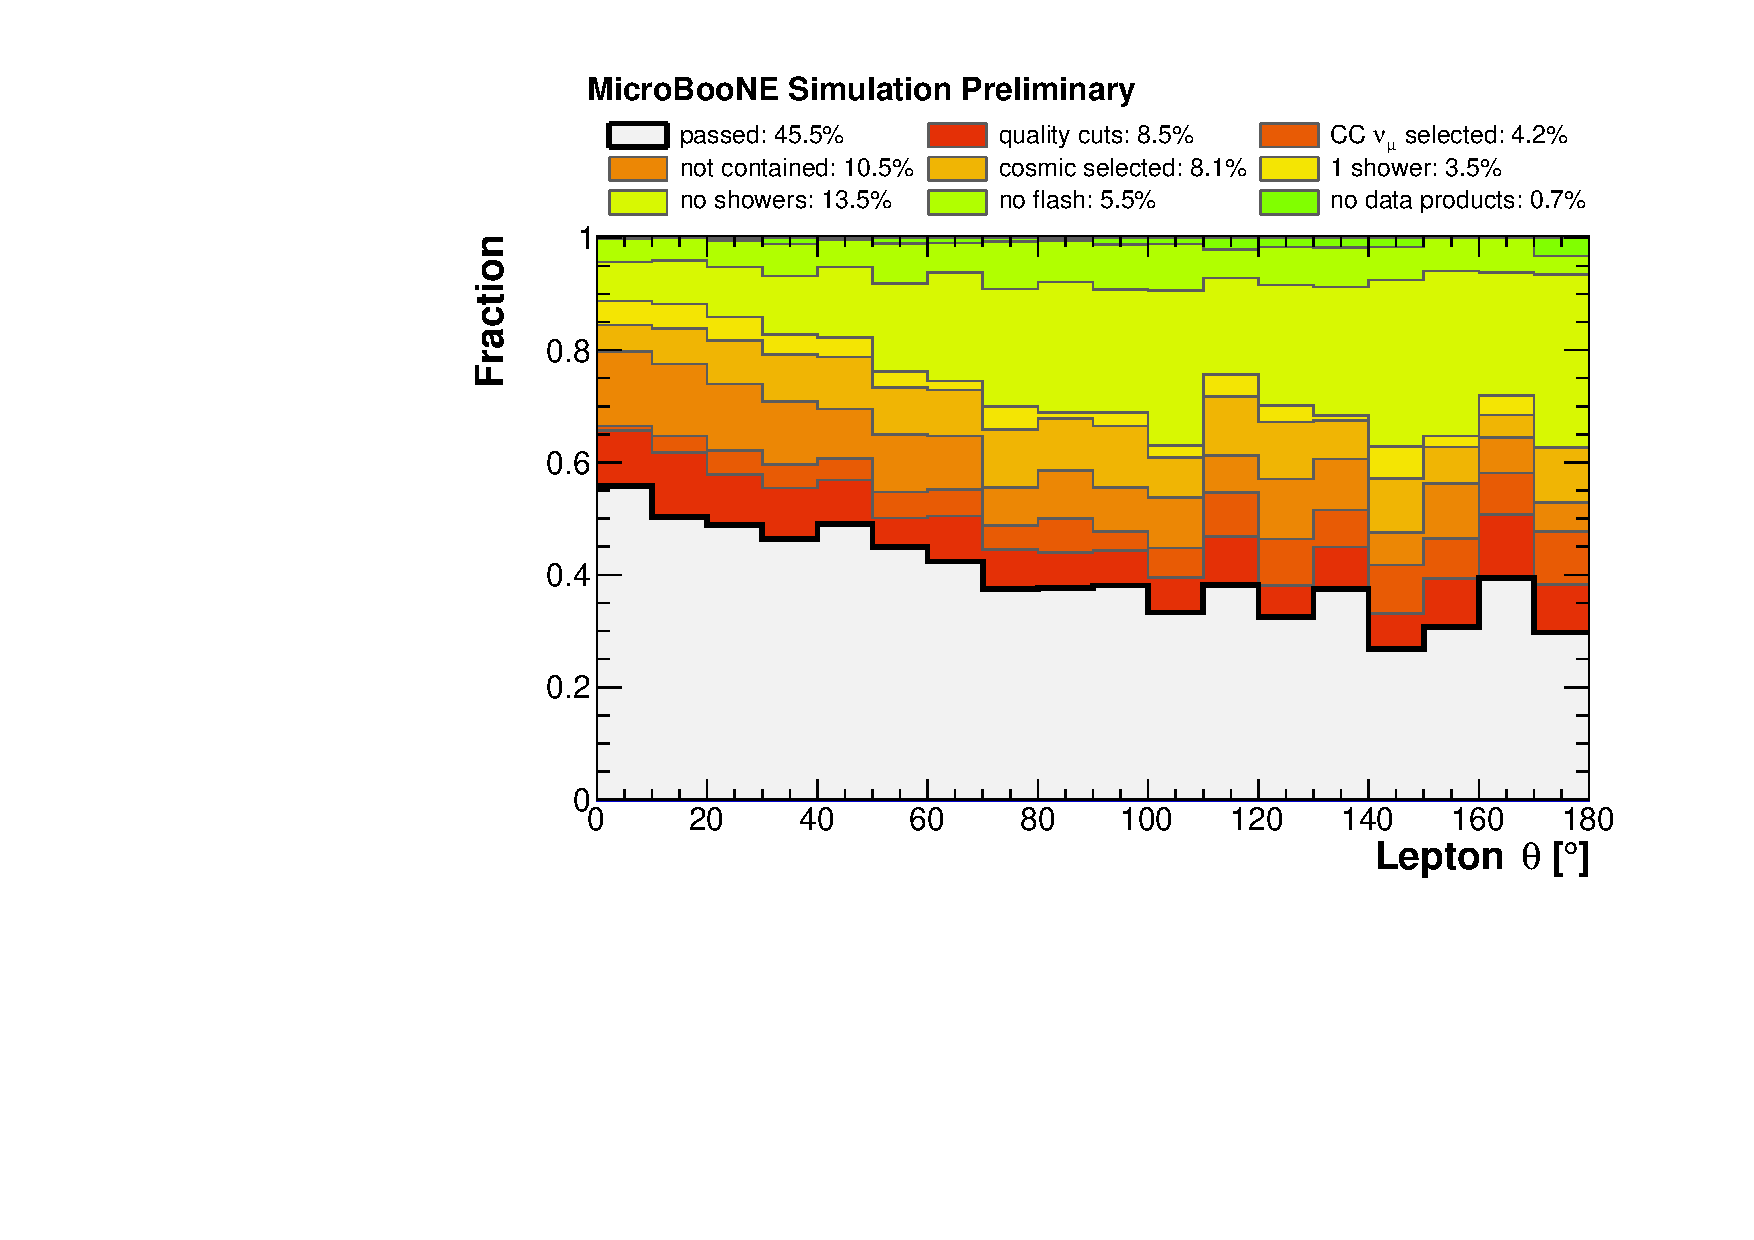
\includegraphics[width=\linewidth]{figures/ineff_theta.pdf}
    \caption{$\theta$ efficiency.} 
  \end{subfigure}
    \begin{subfigure}{0.48\textwidth}
    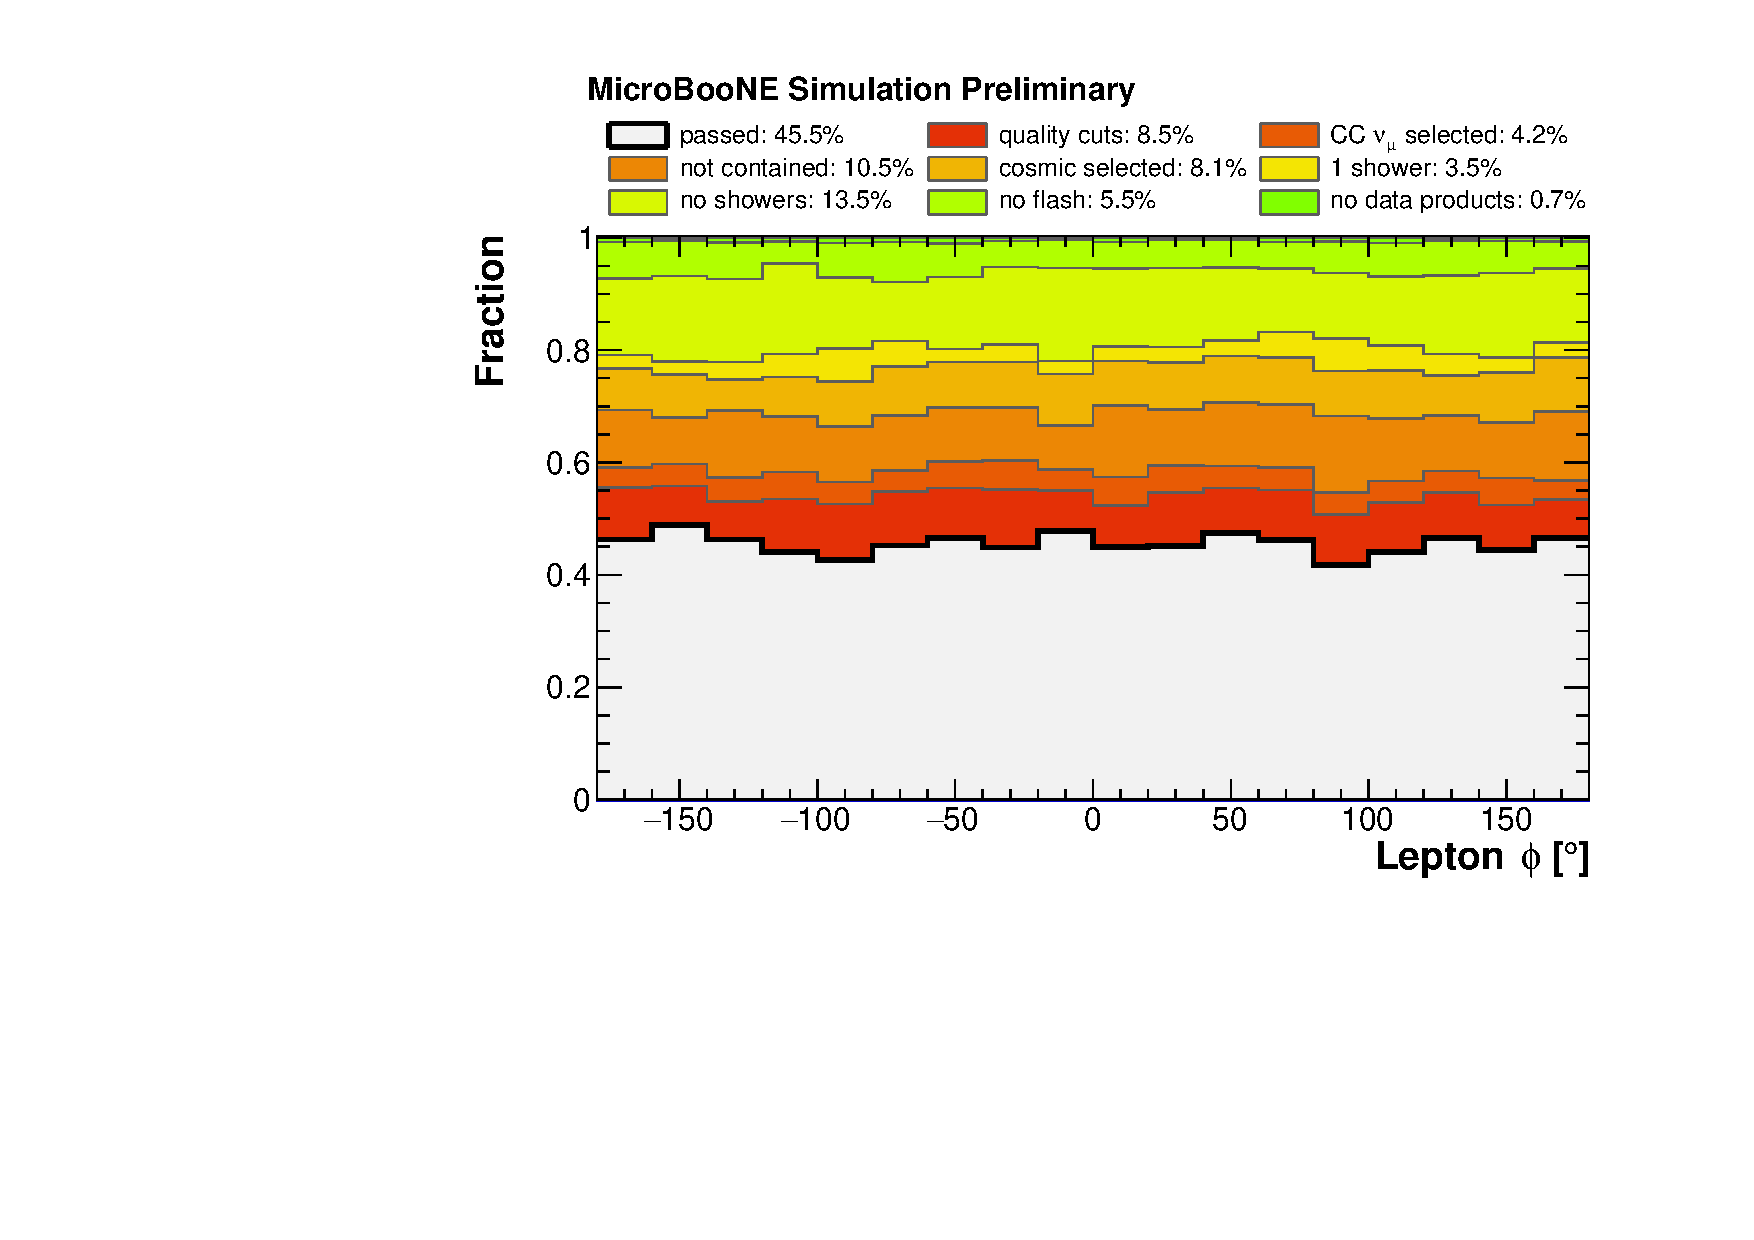
\includegraphics[width=\linewidth]{figures/ineff_phi.pdf}
    \caption{$\phi$ efficiency.} 
  \end{subfigure}
  \caption{Stacked histogram of generated events as a function of the electron $\theta$ (left) and $\phi$ (right) angles, categorised into correctly identified signal events {(\emph{passed})} in grey and different reconstruction or identification failure modes in colour.}
  \label{fig:ineff_angles}
\end{figure}

\subsection{Selection performances in BNB events}\label{sec:numu}
The previous selection efficiency results were performed on a dedicated $\nu_{e}$ CC0$\pi$-Np + cosmic sample. We now look at the selection performances when analysing events coming from the complete set of the events acquired by MicroBooNE from the Booster Neutrino Beam, including all flavours of neutrinos with different fraction (see Figure \ref{fig:bnbflux}). In the \emph{BNB+cosmic} sample every event will have at least one neutrino interacting in the cryostat volume and triggering the detector, plus all the cosmic rays hitting the detector in the same readout window. In the data, however, this is not always true, since the detector can be triggered also by a cosmic ray producing a flash in the optical system during the beam window, without necessarily having a neutrino interaction. In order to estimate this background component, defined as \emph{in-time cosmic rays}, we have used the data sample collected with the \emph{data EXT} trigger.
The background caused by the neutrino interactions happening outside the cryostat has been evaluated using the \emph{dirt} sample.
We divide the selected events (signal and background) into 8 categories:
\paragraph{Signal}
\begin{description}[labelindent=1cm]
\item[Beam intrinsic $\nu_{e}$ CC$0\pi$-Np:] charged-current $\nu_{e}$ neutrino interaction, at least one proton (N > 1), one electron, and no other visible particles above detection threshold. This category represents the signal of our analysis.
\end{description}
\paragraph{Backgrounds}
\begin{description}[labelindent=1cm]
\item[Beam intrinsic $\nu_{e}$ CC:] charged-current $\nu_{e}$ neutrino interaction that is not $\nu_{e}$ CC$0\pi$-Np or where the electron or protons were below the detection threshold defined above.
\item[Beam intrinsic $\nu_{\mu}$:] charged-current $\nu_{\mu}$ neutrino interaction.
\item[Beam intrinsic NC:] neutral current neutrino interaction (both $\nu_{\mu}$ and $\nu_{e}$).
\item[Outside fiducial volume:] neutrino interaction which occurs outside the fiducial volume, but with one or more final-state particles inside in the fiducial volume.
\item[Cosmic contaminated:] neutrino interaction candidate with at least a cosmogenic track or shower, attached to a correctly reconstructed neutrino candidate.
\item[Cosmic:] cosmic ray interaction happening in the same readout window is mistakenly chosen instead of the neutrino interaction in the event. 
\item[Data beam-off]: event with no neutrino interaction, but where a cosmic-ray interaction in time-coincidence with the beam-gate window triggered the event, and activity was selected as a neutrino candidate.
\end{description}

Table \ref{tab:result} shows a summary of the selection algorithm results, with the corresponding number of events for each category.
%The numbers correspond to an exposure of the MicroBooNE detector of \num{4.34e19} protons on target (POT). This is equivalent to the amount of data analysed here, which is a subset of the data collected from February to April 2016.

\begin{table}[htbp]
   \centering
      \caption{Summary of the selection results, showing the contribution of each event category, for a MicroBooNE exposure of \num{4.34e19} POT. Efficiency uncertainties are statistical only. {For the \emph{Cosmic contaminated} category the number of generated events correspond to the number of neutrino interactions inside the cryostat. For the \emph{Cosmic} category, it corresponds to the total number of simulated neutrino interactions, both inside and outside the cryostat.}}\label{tab:result}
   \begin{tabular}{lrrr}
     \toprule
     Category & Generated & Selected & Efficiency [\%]\\
     \midrule

     \textbf{$\nu_{e}$ CC0$\pi$-Np (signal)}  & $33.8$    & $15.4$  & $45.5\pm0.5$\\
     $\nu_{e}$ CC                             & $39.5$    & $15.4$  & $39.0\pm0.5$\\
     Beam intrinsic $\nu_{\mu}$               & $10905.9$ & $488.9$ & $4.5\pm0.2$\\
     Beam intrinsic NC                        & $3532.8$  & $329.5$ & $9.3\pm0.2$\\
     Outside fid. vol.                        & $36634.6$ & $79.0$  & $0.2\pm0.1$\\
     Data off-beam                            & $123070.2$ & $1593.4$ & $1.3\pm0.1$\\
     Cosmic contaminated                      & $14706.4$  & $376.1$  & $2.5\pm0.1$\\ 
     Cosmic                                   & $51356.1$  & $489.4$  & $0.8\pm0.1$\\

     \bottomrule
   \end{tabular}

\end{table}

At this point, all selected events have a neutrino interaction candidate with one or more tracks and one or more showers associated with the interaction vertex. Since we use two different methods to measure the energy of the tracks and the energy of the showers (see Section \ref{sec:energyreco}), it is necessary to verify the agreement between the shower multiplicity and track multiplicity distributions in data and Monte Carlo. Figure \ref{fig:multiplicity} shows that the two distributions agree within the systematic uncertainties, whose evaluation is described in Section \ref{sec:systematics}.

\begin{figure}[htbp]
\centering
  \begin{subfigure}{0.49\textwidth}
    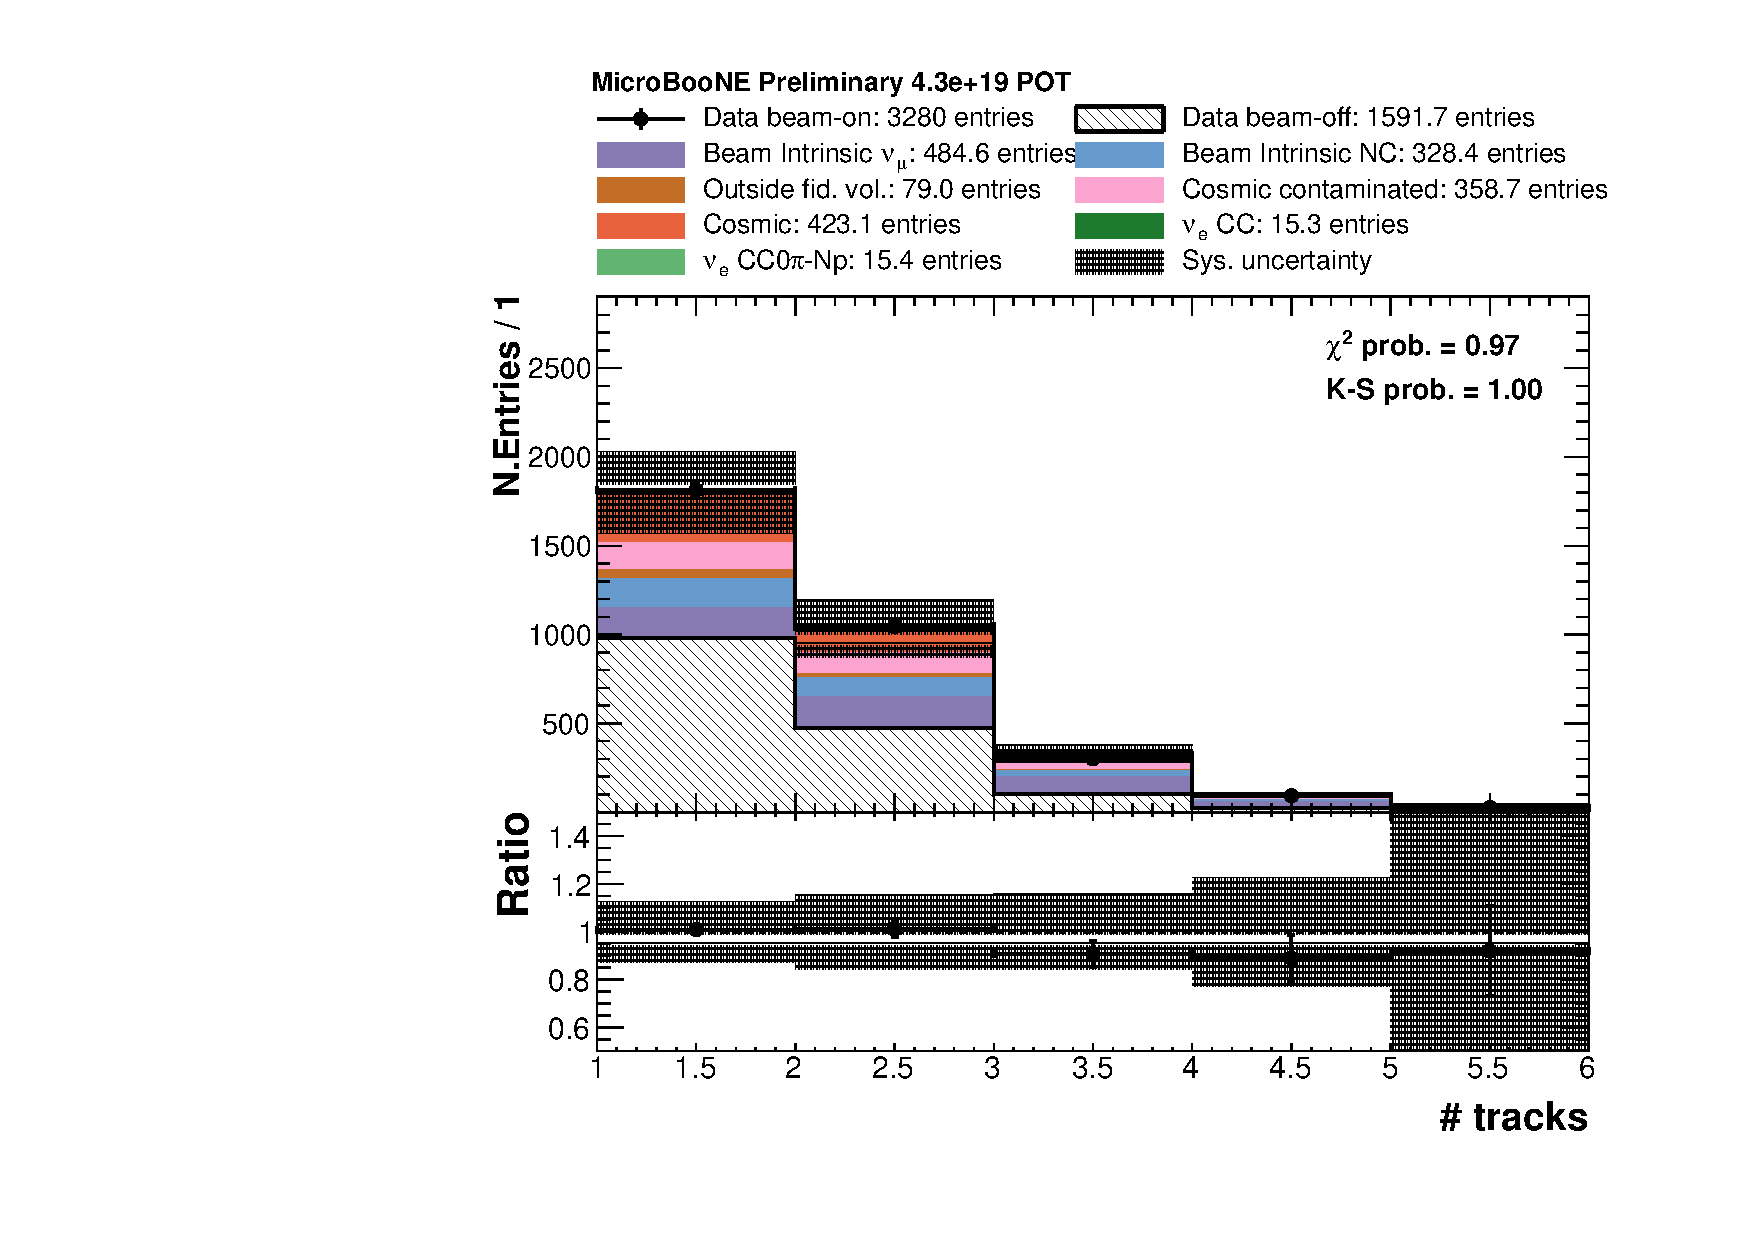
\includegraphics[width=\linewidth]{figures/n_tracks.pdf}
    \caption{Track multiplicity.} 
  \end{subfigure}\hfill
    \begin{subfigure}{0.49\textwidth}
    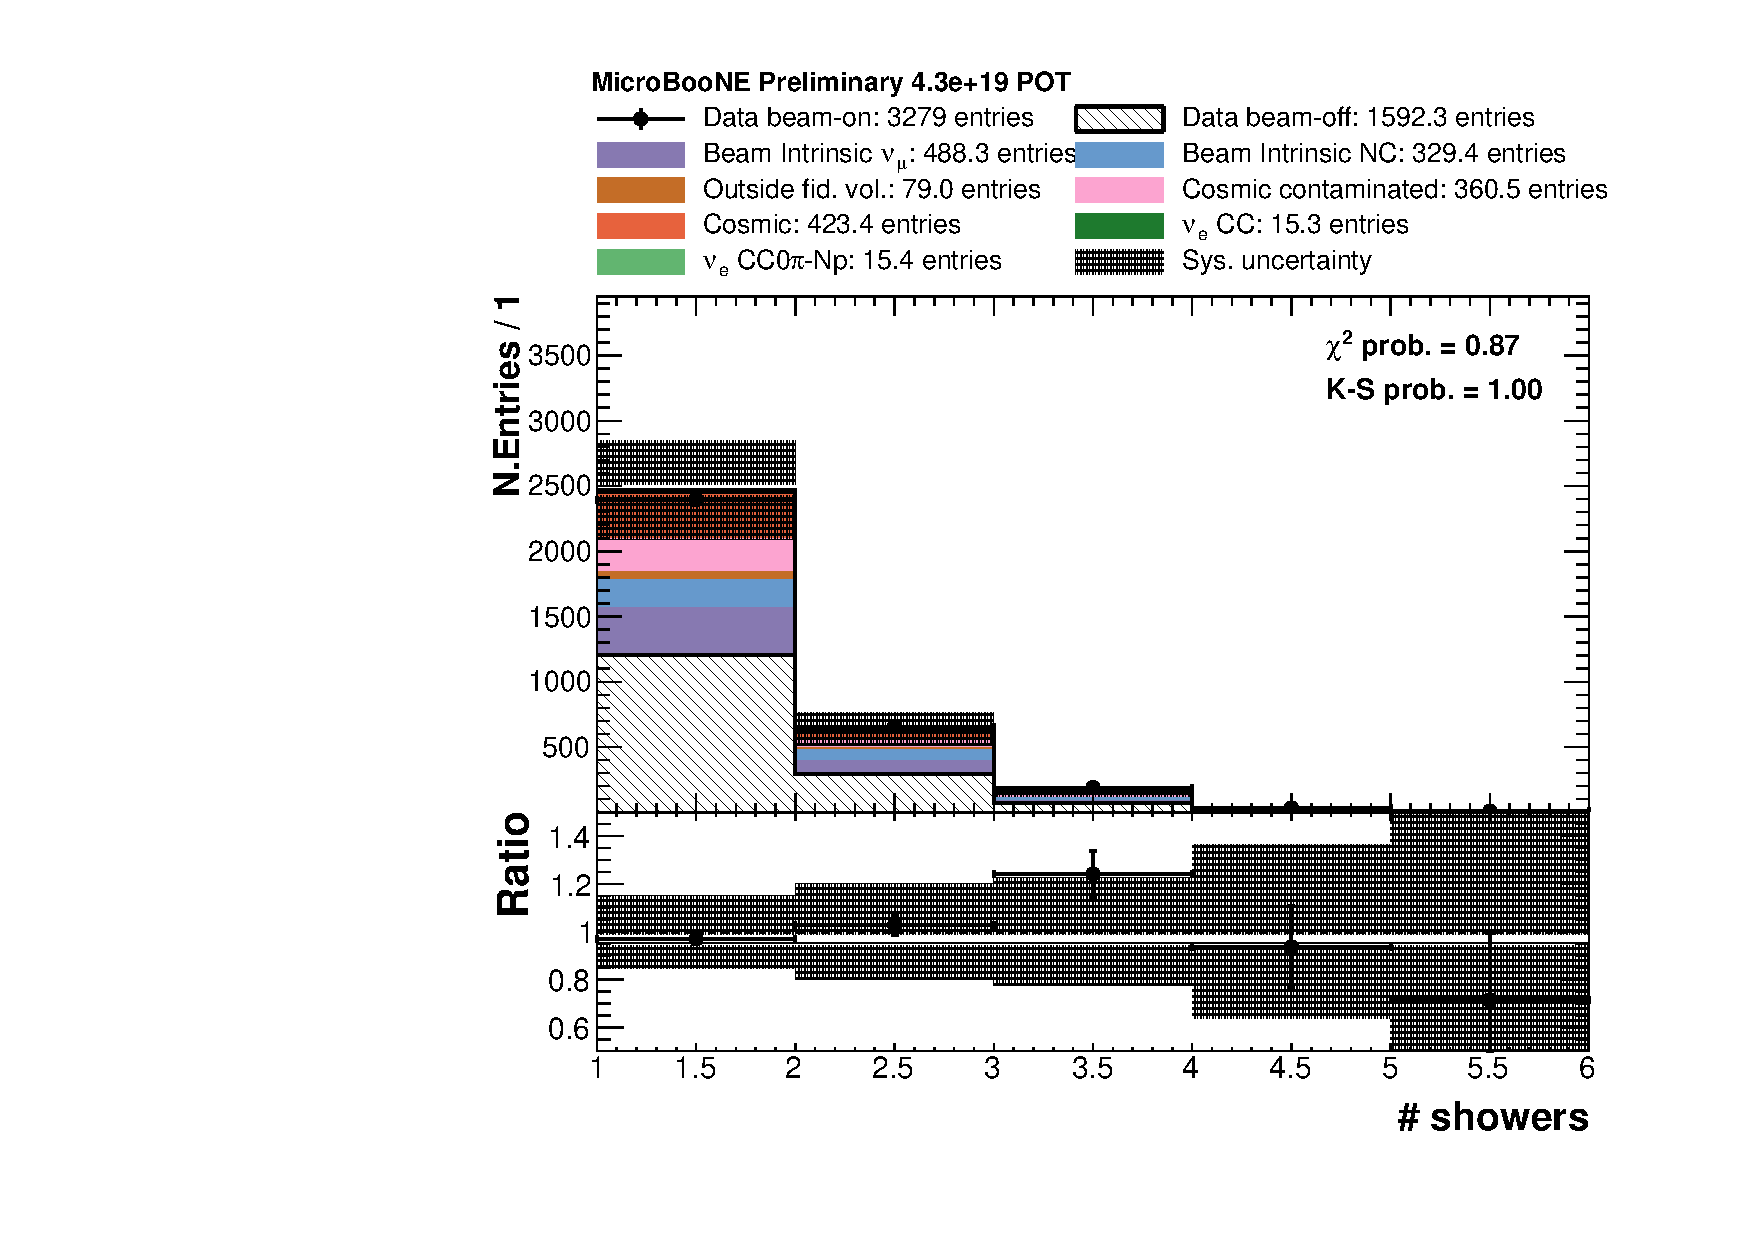
\includegraphics[width=\linewidth]{figures/n_showers.pdf}
    \caption{Shower multiplicity.} 
  \end{subfigure}
  \caption{Distributions of the track and shower multiplicities in data and Monte Carlo simulation.}\label{fig:multiplicity}
\end{figure}

The agreement between data and simulation is also verified in the angular distributions of the reconstructed showers objects, shown in Figure \ref{fig:thetaphi}. As expected, the neutrino distributions are mostly constant as a function of the azimuthal angle $\phi$ and peaked at low inclination angle $\theta$ values, since the interactions are mostly forward going. The inclination angle $\theta$ distribution agrees within the uncertainties both for shape and normalisation. The azimuthal angle $\phi$ distribution shows a slight disagreement around $\phi = 0^{\circ}$ and $\phi = \pm180^{\circ}$. This is caused by an imprecise signal simulation that predominantly affects tracks moving exactly towards or away from the anode \cite{Adams:2018gbi}. This effect is taken into account in the Dynamic Induced Charge detector systematic sample (Section \ref{sec:systematics}). 

Figure \ref{fig:thetaphi_pdg} shows the angular distributions classified according to the primary particle that generated the shower (in the case of a Michel electron the shower is placed in the muon category). Each entry in the histogram correspond to a reconstructed shower, so it is possible to have more than one entry per event. As expected, the $\theta$ distribution is peaked at low angles, since neutrino interactions are mostly forward going. The $\phi$ distribution is mainly flat for neutrino-induced particles (electrons, photons) and with two peaks at $\pm90^{\circ}$ for mostly-vertical cosmic-induced particles (mainly muons). In this case, the data points correspond to the bin-by-bin statistical subtraction of the beam-on and beam-off entries.

\begin{figure}[htbp]
\centering
  \begin{subfigure}{0.49\textwidth}
    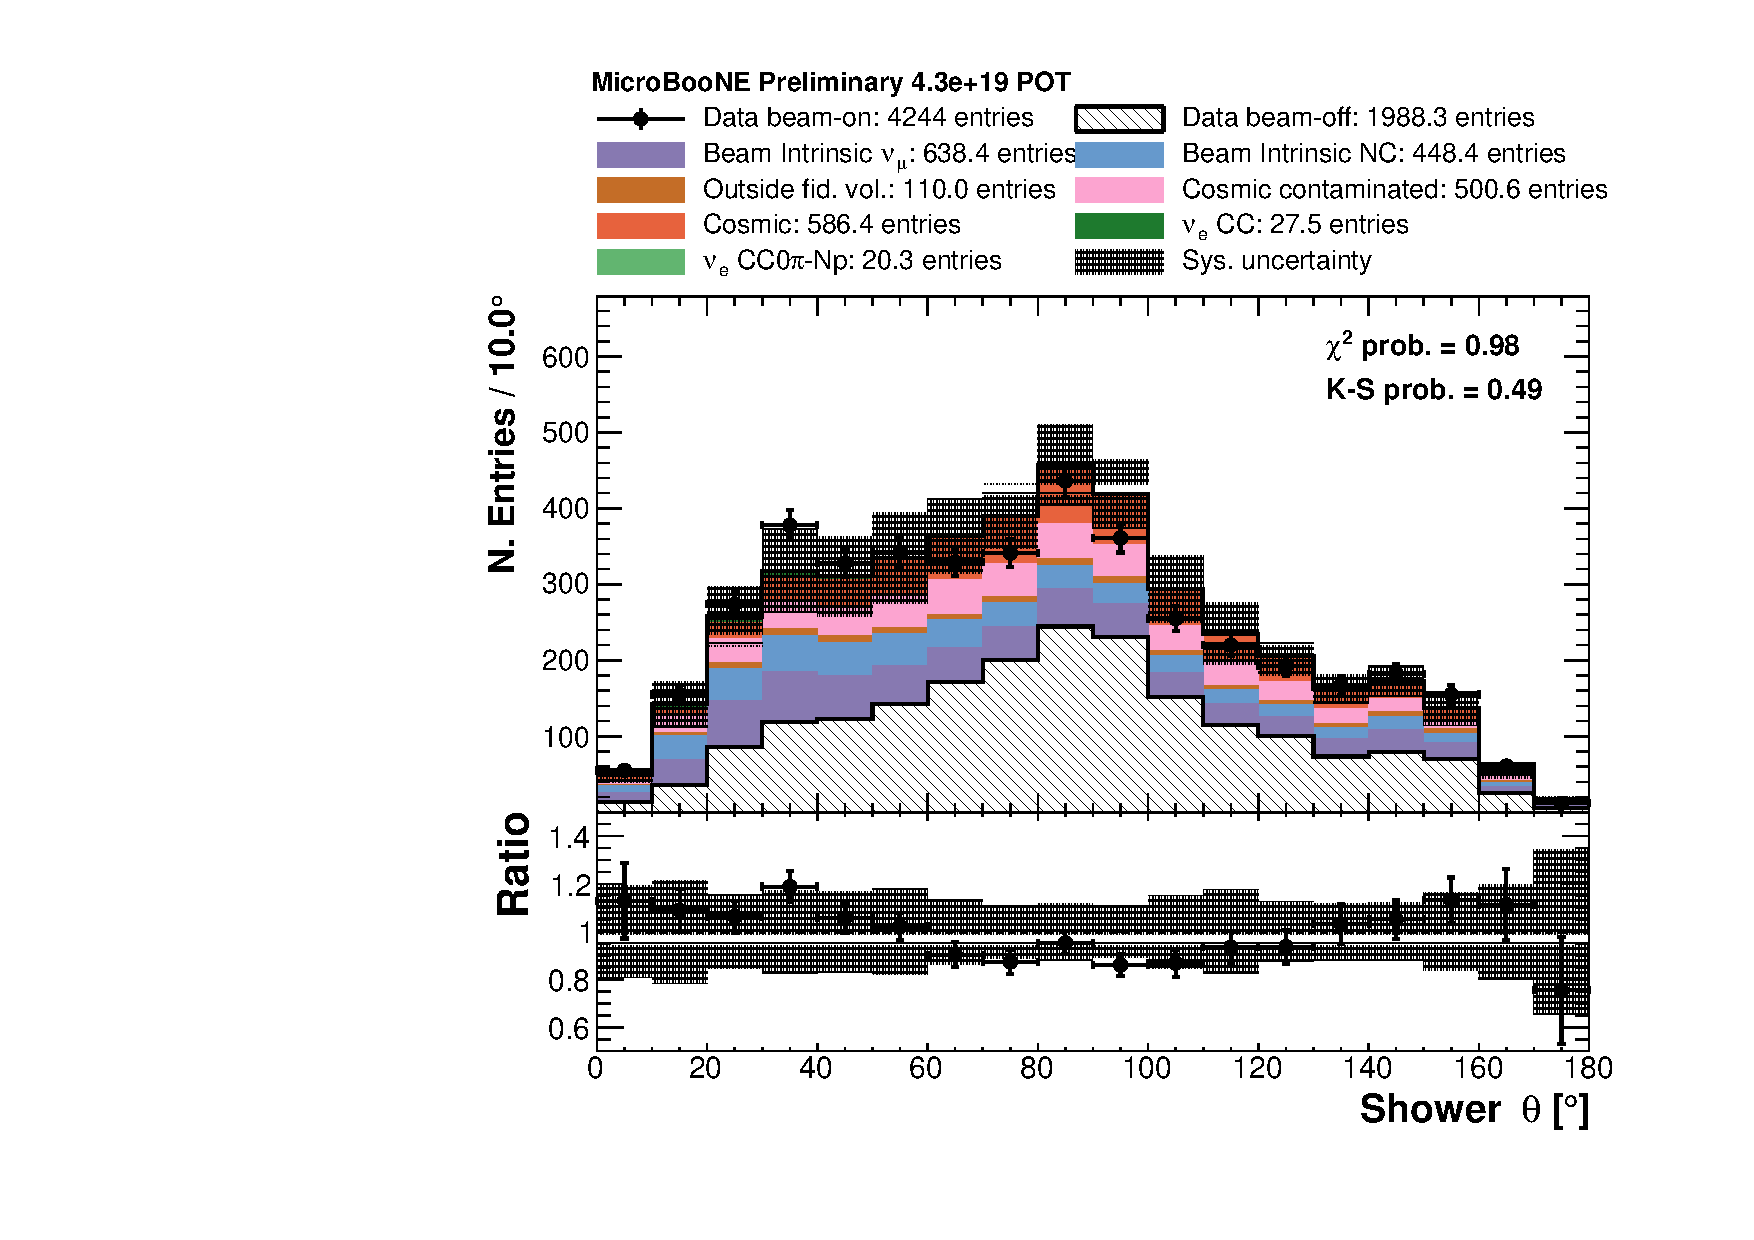
\includegraphics[width=\linewidth]{figures/h_shower_theta.pdf}
    \caption{Inclination angle $\theta$.} 
  \end{subfigure}\hfill
    \begin{subfigure}{0.49\textwidth}
    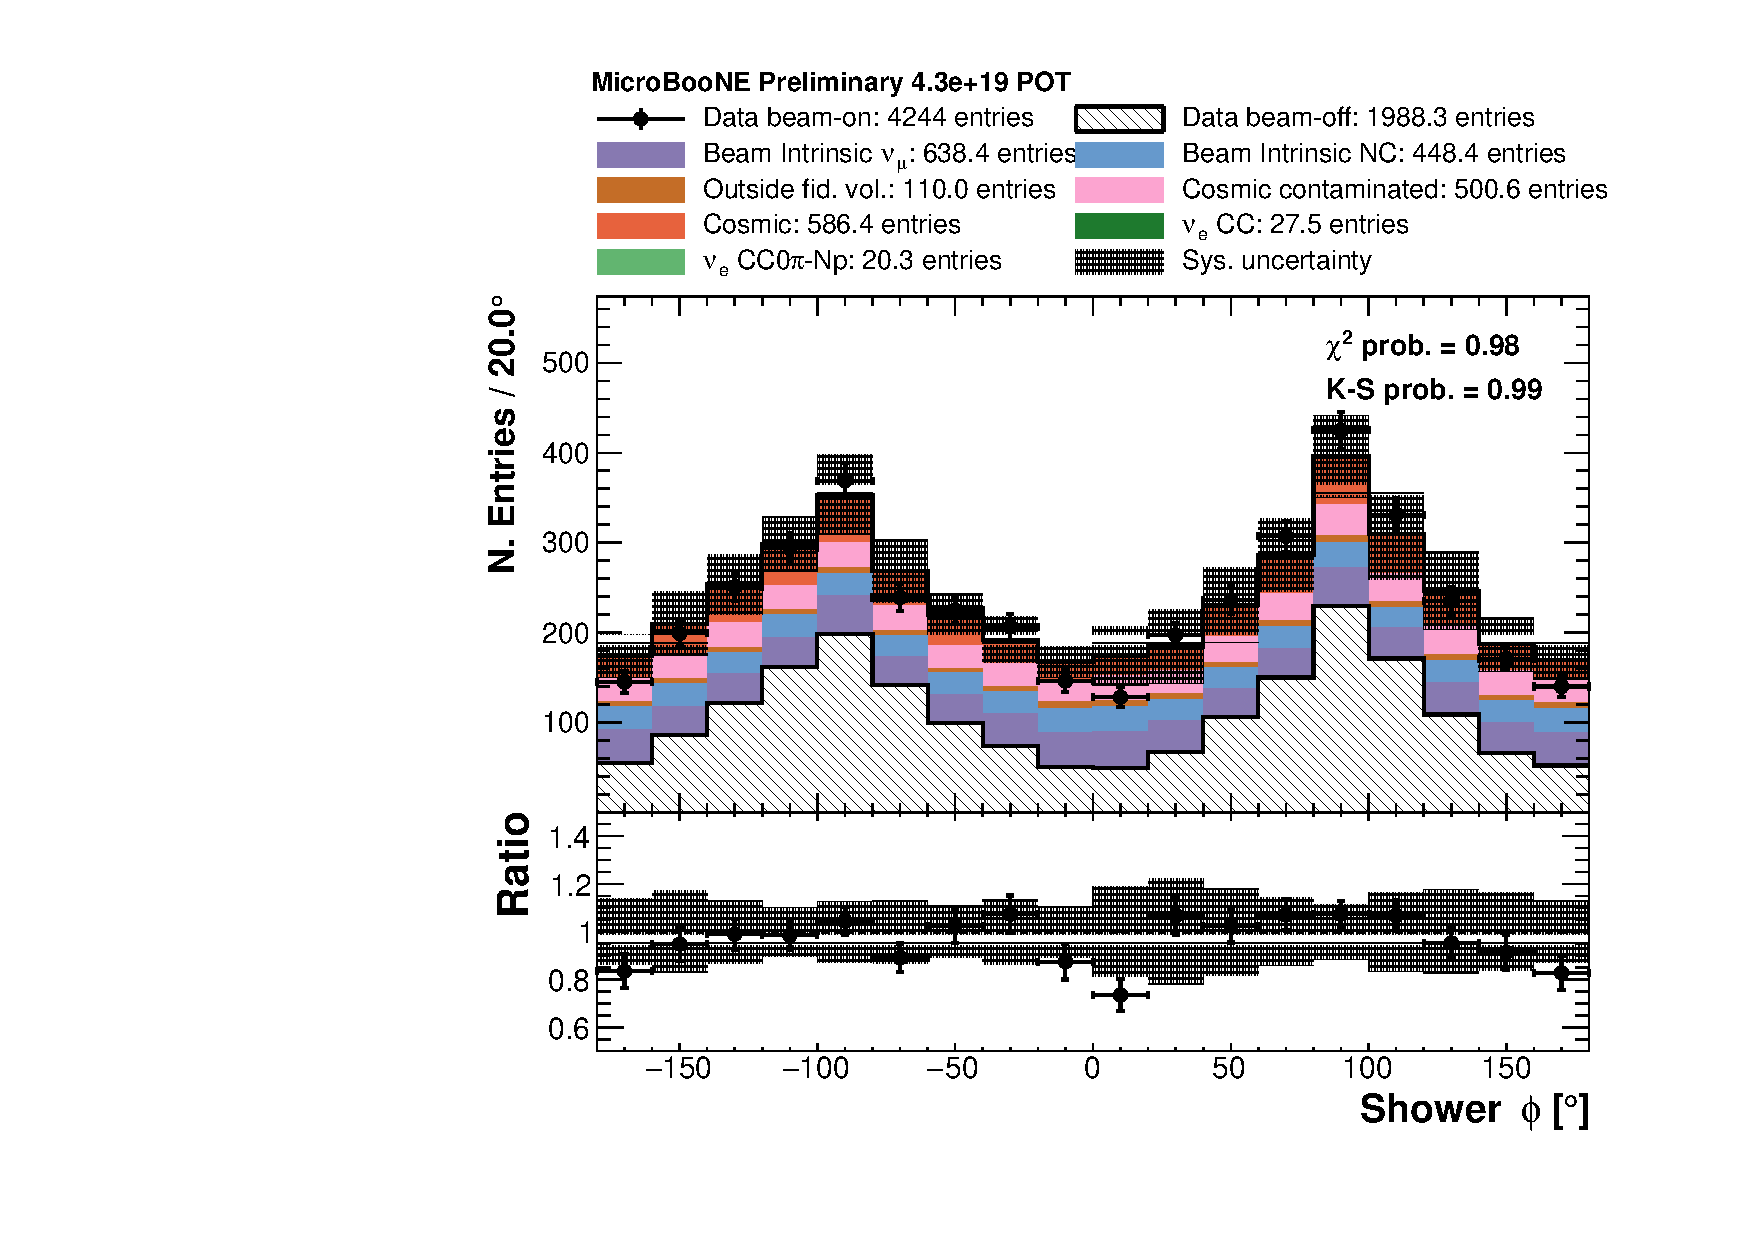
\includegraphics[width=\linewidth]{figures/h_shower_phi.pdf}
    \caption{Azimuth angle $\phi$.} 
  \end{subfigure}
  \caption{Distributions of the inclination angle $\theta$ and the azimuthal angle $\phi$ of the reconstructed showers in the selected events for each event category. The black points represent the data with statistical uncertainties. The coloured stacked histograms represent the simulated events, with the hatched histogram corresponding to the data beam-off sample. The shaded area represents the systematic uncertainty. The bottom part of the plot shows the ratio between the data beam-on events and the stacked histograms.}\label{fig:thetaphi}
\end{figure}

\begin{figure}[htbp]
\centering
  \begin{subfigure}{0.49\textwidth}
    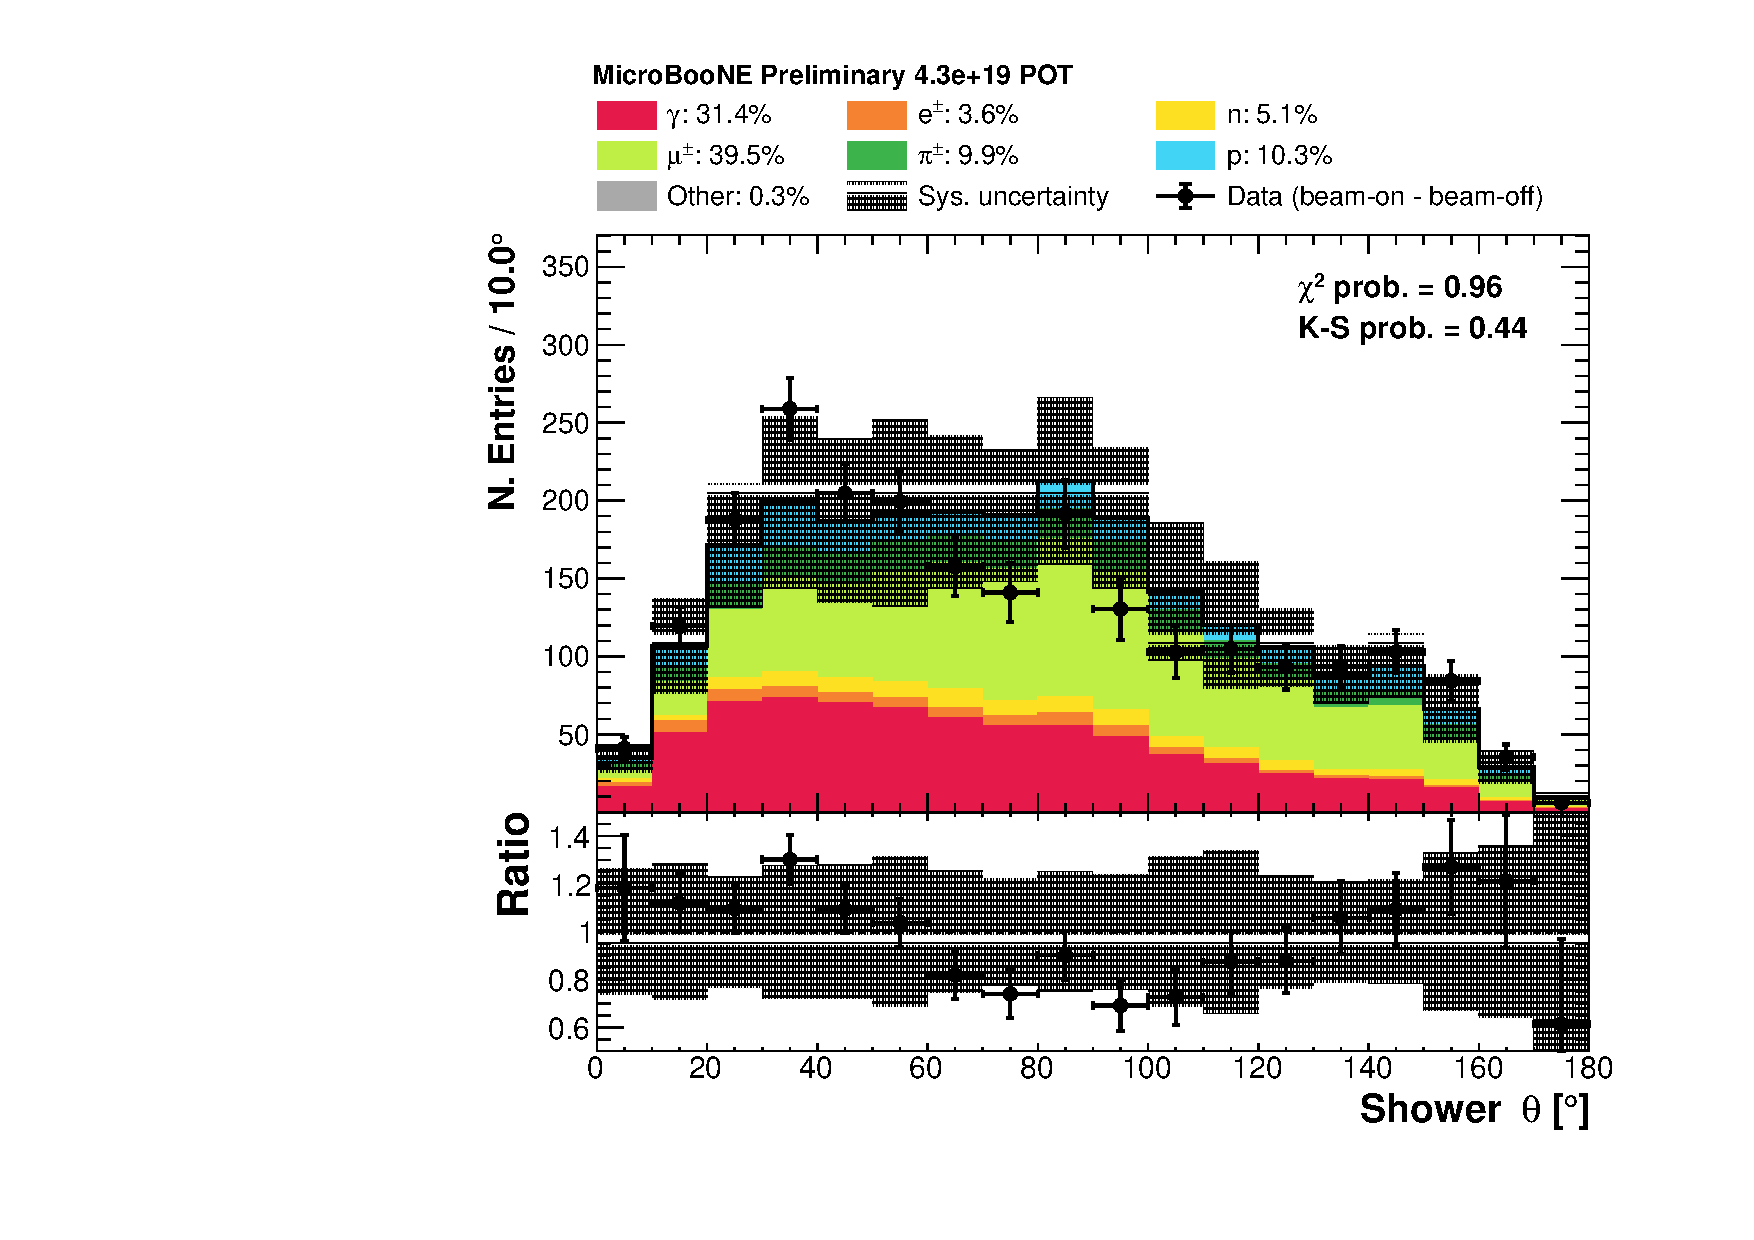
\includegraphics[width=\linewidth]{figures/h_shower_theta_pdg.pdf}
    \caption{Inclination angle $\theta$.}\hfill
  \end{subfigure}
    \begin{subfigure}{0.49\textwidth}
    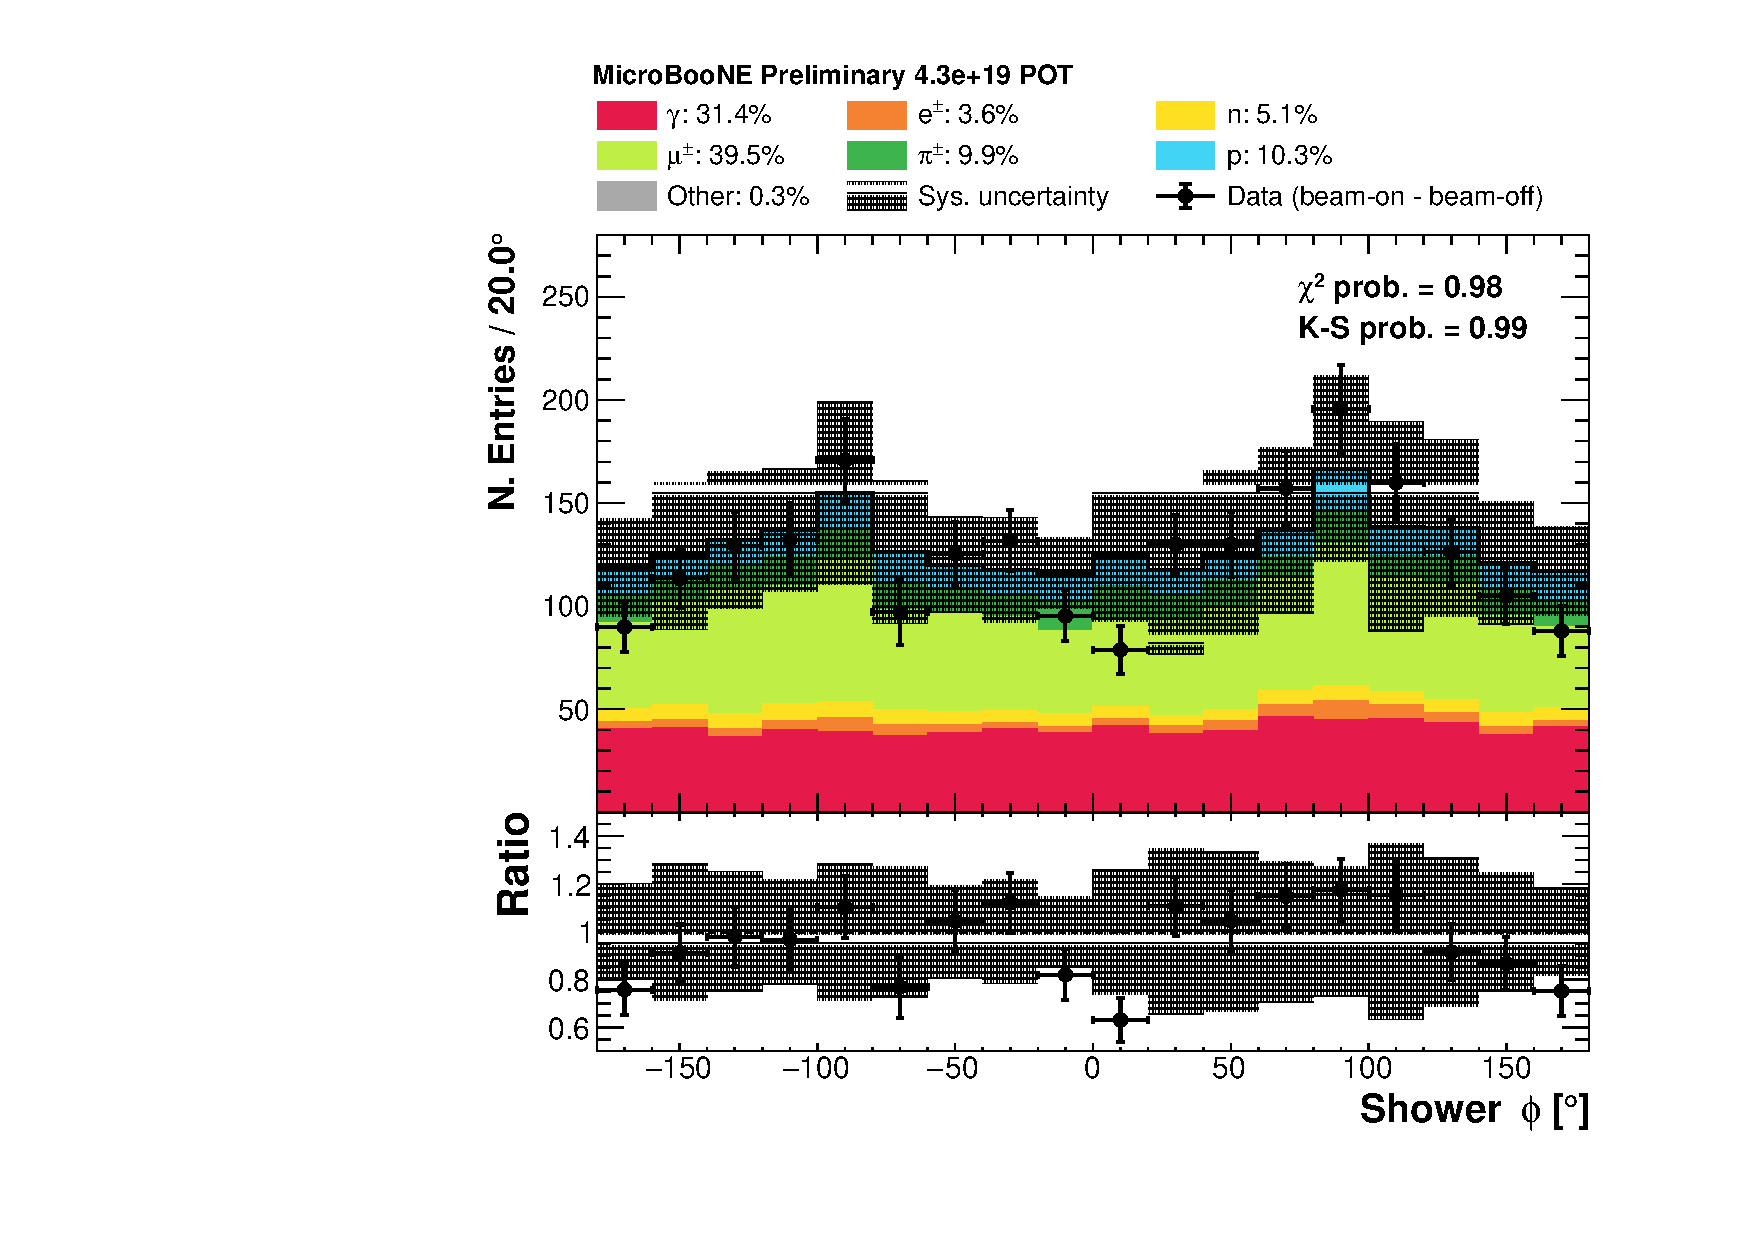
\includegraphics[width=\linewidth]{figures/h_shower_phi_pdg.pdf}
    \caption{Azimuth angle $\phi$.} 
  \end{subfigure}
  \caption{Distributions of the inclination angle $\theta$ and the azimuthal angle $\phi$ of the reconstructed showers, classified according to the primary particle that generated them. The black points represent the statistically subtraction of the data beam-off events from the data beam-on events. The coloured stacked histograms represent the simulated events. The shaded area represents the systematic uncertainty. The bottom part of the plot shows the ratio between the statistical subtraction and the stacked histograms.}\label{fig:thetaphi_pdg}
\end{figure}

A small fraction of the data events was also visually inspected: Figure \ref{fig:evds} shows three event displays of data events compatible with a $\nu_{e}$ CC0$\pi$-Np interaction. 

\begin{figure}[htbp]
\centering
  \begin{subfigure}{0.45\textwidth}
  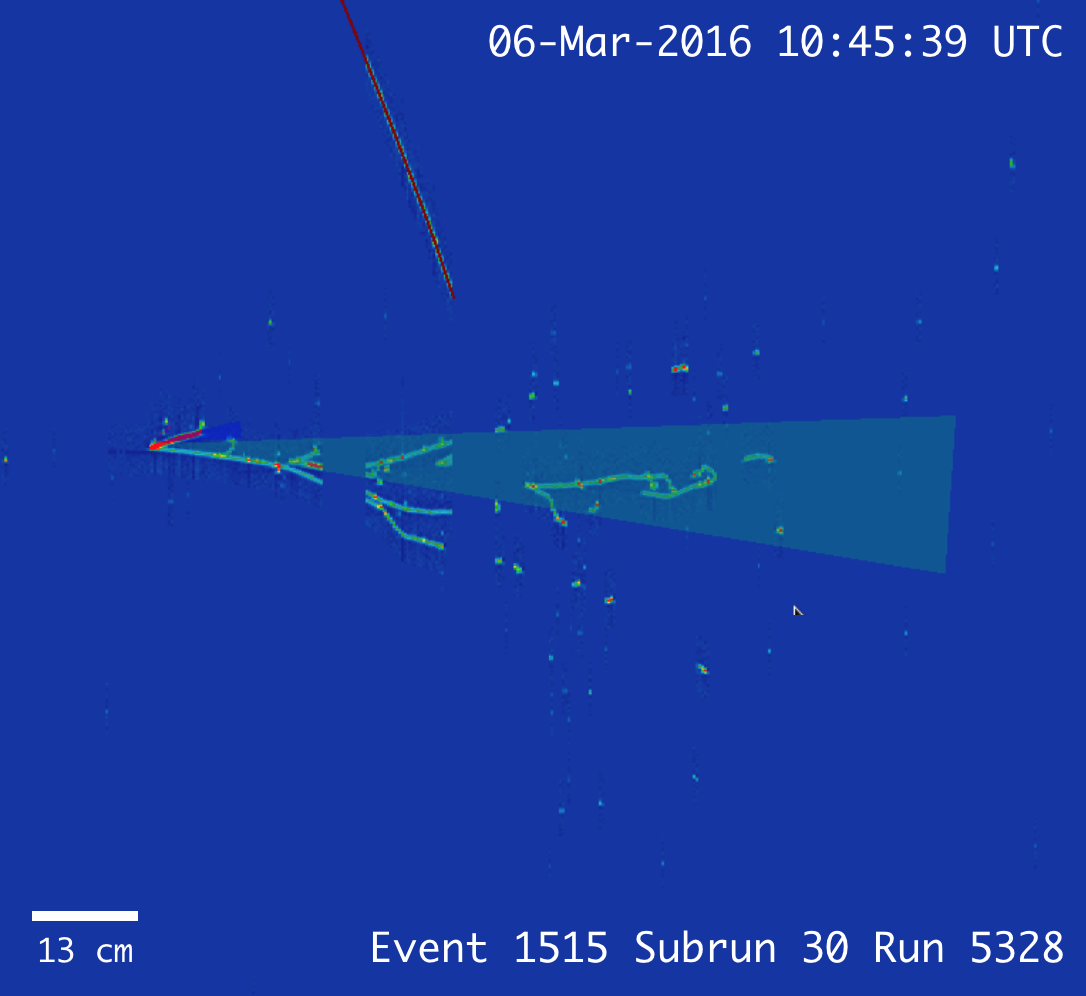
\includegraphics[width=\linewidth]{figures/data3.png}
    \caption{Event 1515, Subrun 30, Run 5328}\end{subfigure}
  \hfill\begin{subfigure}{0.45\textwidth}	
  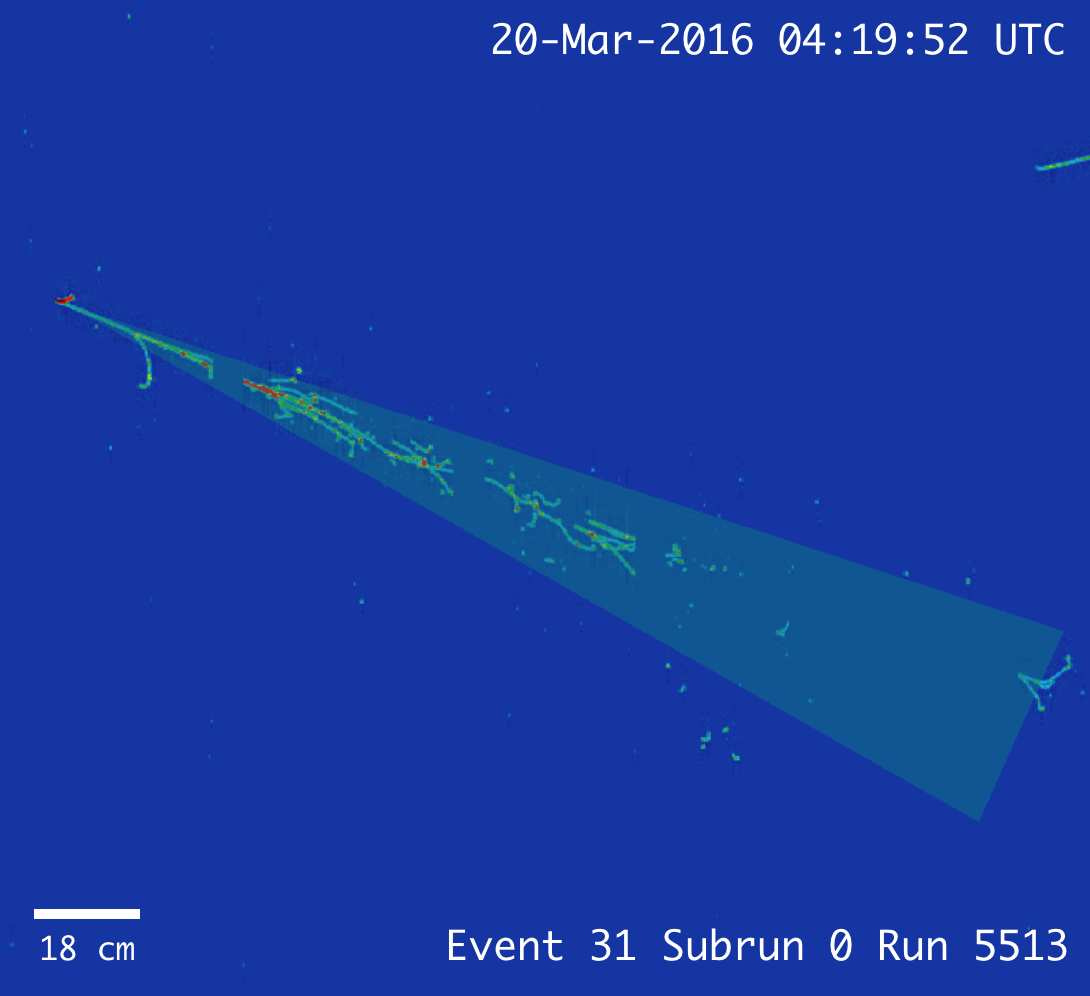
\includegraphics[width=\linewidth]{figures/data2.png}
  \caption{Event 31, Subrun 0, Run 5513}
\end{subfigure}
\vspace{1em}

  \begin{subfigure}{0.45\textwidth}	
  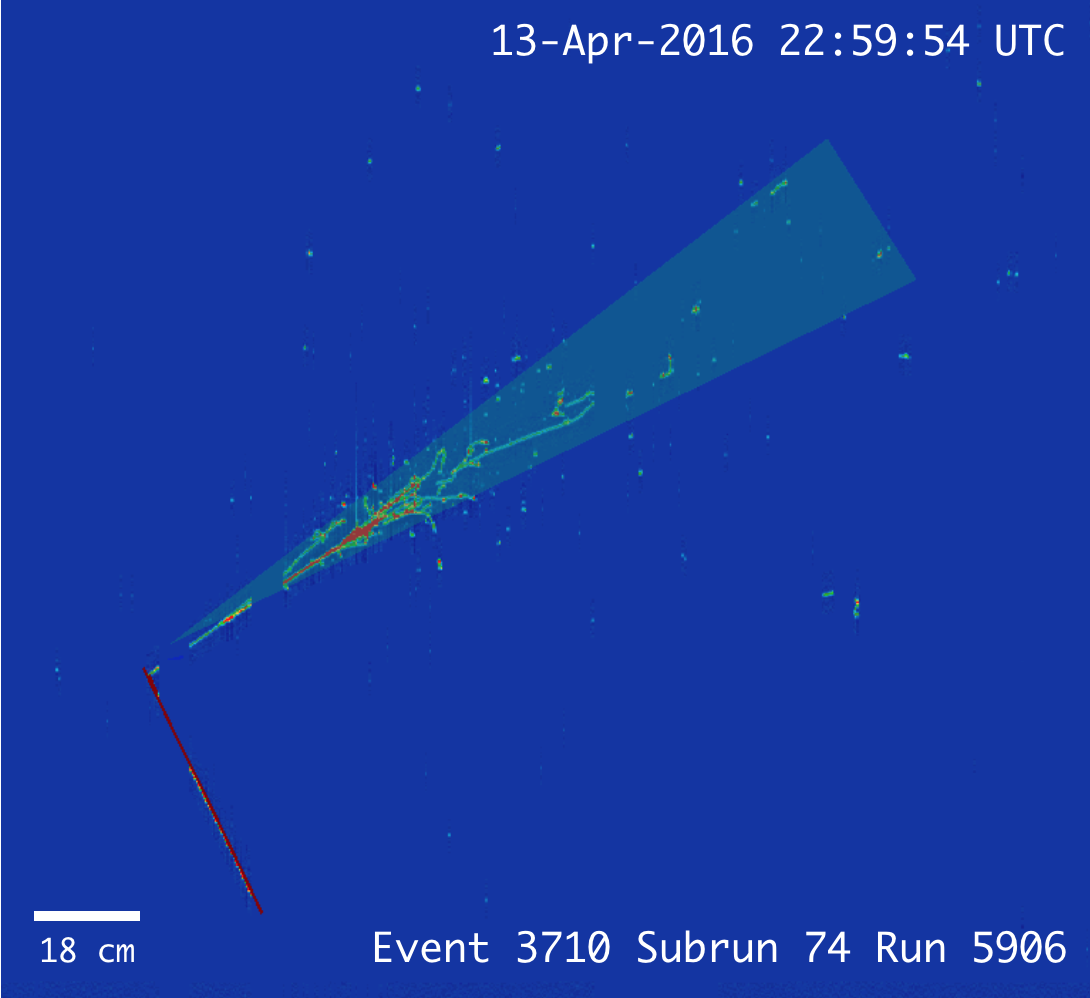
\includegraphics[width=\linewidth]{figures/data1.png}
  \caption{Event 3710, Subrun 74, Run 5906}
\end{subfigure}

  \caption{Event displays of the collection plane of three $\nu_{e}$-like data events selected by our algorithm. The gaps are caused by the presence of missing wires. The red lines correspond to reconstructed track-like objects and the green cones correspond to reconstructed shower-like objects. }
  \label{fig:evds}
\end{figure}


\section{Calorimetry}\label{sec:energyreco}
\subsection{Scope of the energy reconstruction}
In this analysis we restrict ourselves to the measurement of the deposited energy in the TPC of the visible particles in the final state of the $\nu_e$ CC0$\pi$-Np neutrino interaction. Our signal has in its final state, by definition, one electron and at least one proton, with no other visible particles. The energy of the electron is measured by converting the reconstructed charge of all the shower-like objects into deposited energy, as described in Section \ref{sec:showerenergy}. The energy of the protons, instead, can be measured by converting the track length of the reconstructed tracks into deposited energy, using the tabulated stopping power of protons in the liquid argon, with the procedure described in \ref{sec:protonenergy}. The total reconstructed energy corresponds to the sum of the reconstructed energies, corrected by the calibration factors calculated below, and is referred to as $E_{\mathrm{corr}}$. This quantity is then compared with the total kinetic energy of the particles above detection thresholds and corrected by a calibration factor to obtain an estimate of the deposited energy $E_{\mathrm{deposited}}$ (Section \ref{sec:deposited}).


\subsection{Electron energy reconstruction and calibration}\label{sec:showerenergy}
The reconstructed energy $E_{\mathrm{reco}}^{e}$ of a shower-like object is measured converting the charge of the associated hits into deposited energy in the TPC. It is calculated by multiplying the reconstructed charge ($e^{-}_{\mathrm{reco}}$) from hits associated with the reconstructed shower by the calibration factor \cite{Acciarri:2017sjy}:
\begin{equation}
\frac{E_{\mathrm{reco}}^{e} \mathrm{(MeV)}}{e^{-}_{\mathrm{reco}}} = 1.01\frac{e^-}{e^{-}_{\mathrm{reco}}} \times \frac{23.6~\mathrm{eV}}{e^-} \times 10^{-6} \frac{\mathrm{MeV}}{\mathrm{eV}} \times \frac{1}{R} = 3.85\times10^{-5},\label{eq:calib}
\end{equation}
where:
\begin{itemize}

\item the correction factor $1.01\frac{e^-}{e^{-}_{\mathrm{reco}}}$ is obtained measuring the true number of collected electrons $e^{-}$ on the wires using a sample of stopping muons, fitting the $dE/dx$ vs. residual range to values for argon as tabulated by the PDG \cite{PhysRevD.98.030001};
\item $\frac{23.6~\mathrm{eV}}{e^-}$ is the work function for ionizing an argon atom \cite{Shibamura:1975zz};
\item $R = 0.62$ is the recombination factor obtained with the Modified Box Model \cite{Acciarri:2013met} at MicroBooNE's electric field of 270~V/cm assuming an energy loss per length $dE/dx=2.3$~MeV/cm.
\end{itemize}

The reconstructed energy is obtained summing the energy of each hit from the reconstructed showers produced by a simulated electron in the collection plane, produced by a $\nu_{e}$ CC0$\pi$-Np interaction. The starting point of the simulated electron and the starting point of the reconstructed showers are required to be within the fiducial volume. 
Figure \ref{fig:ecalib} shows the calibration slope necessary to convert the electron reconstructed energy $E_{\mathrm{reco}}^{e}$ into true electron energy $E^{e}$. The true energy spectrum has been divided into 10 bins of equal size in the 30-2030~MeV range. Since the reconstructed energy distributions in each true energy bin are asymmetric, the data points are obtained fitting the distributions with a GaussExp function \cite{Das:2016stf}, in order to estimate the most probable value (MPV). The GaussExp function consists of an exponential tail stitched to a Gaussian core and it is often use to measure lossy processes such as the energy reconstructed in a calorimeter. The coordinate on the $E^{e}$ axis are given by the mean of the true energy distribution for each bin. The vertical error bars correspond to the full width at half maximum (FWHM) of the fitted function. The true energy distribution and the reconstruction energy distribution for every bin are shown in Figure \ref{fig:e_spectra}.

\begin{figure}[htbp]
\centering
\begin{overpic}[width=0.95\linewidth]{figures/e_spectra.pdf}
\end{overpic}
% 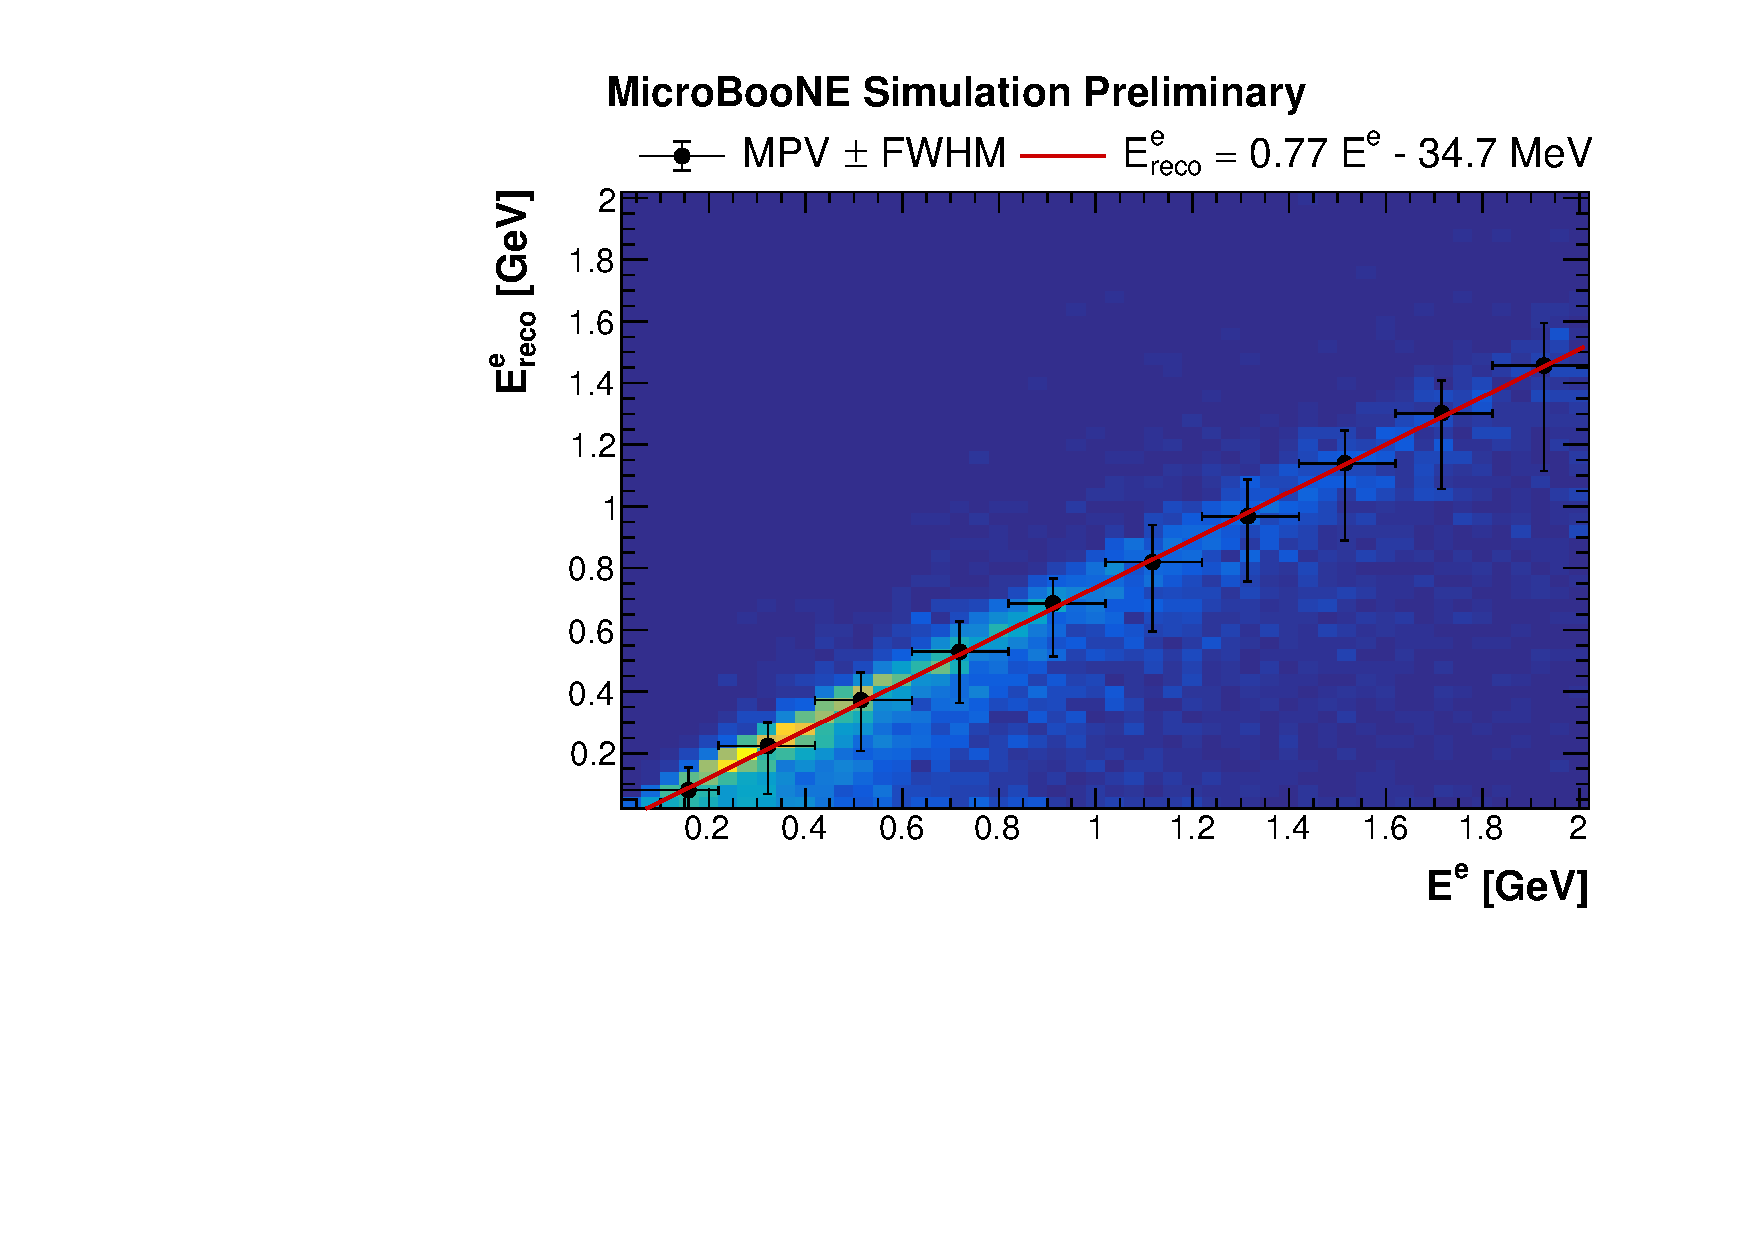
\includegraphics[width=0.65\columnwidth]{figures/ecalib.pdf}
\caption{Reconstructed and true energy distribution for 10 intervals of equal size in the 30-2030 MeV energy range. The reconstructed energy distribution have been fitted with a GaussExp function.}
\label{fig:e_spectra}
\end{figure}


The linear fit of the most probable value points, shown in Figure \ref{fig:ecalib} gives:
\begin{equation}
E_{\mathrm{reco}}^{e} = 0.77~E^{e} - 34.7~\mathrm{MeV}.
\end{equation}
The energy of the shower, corrected by the calibration factor is then defined as:
\begin{equation}
E_{\mathrm{corr}}^{e} = (E_{\mathrm{reco}}^{e} + 34.7~\mathrm{MeV})/0.77.
\end{equation}

\begin{figure}[htbp]
\centering
\begin{overpic}[width=0.7\linewidth]{figures/ecalib.pdf}
\end{overpic}
% 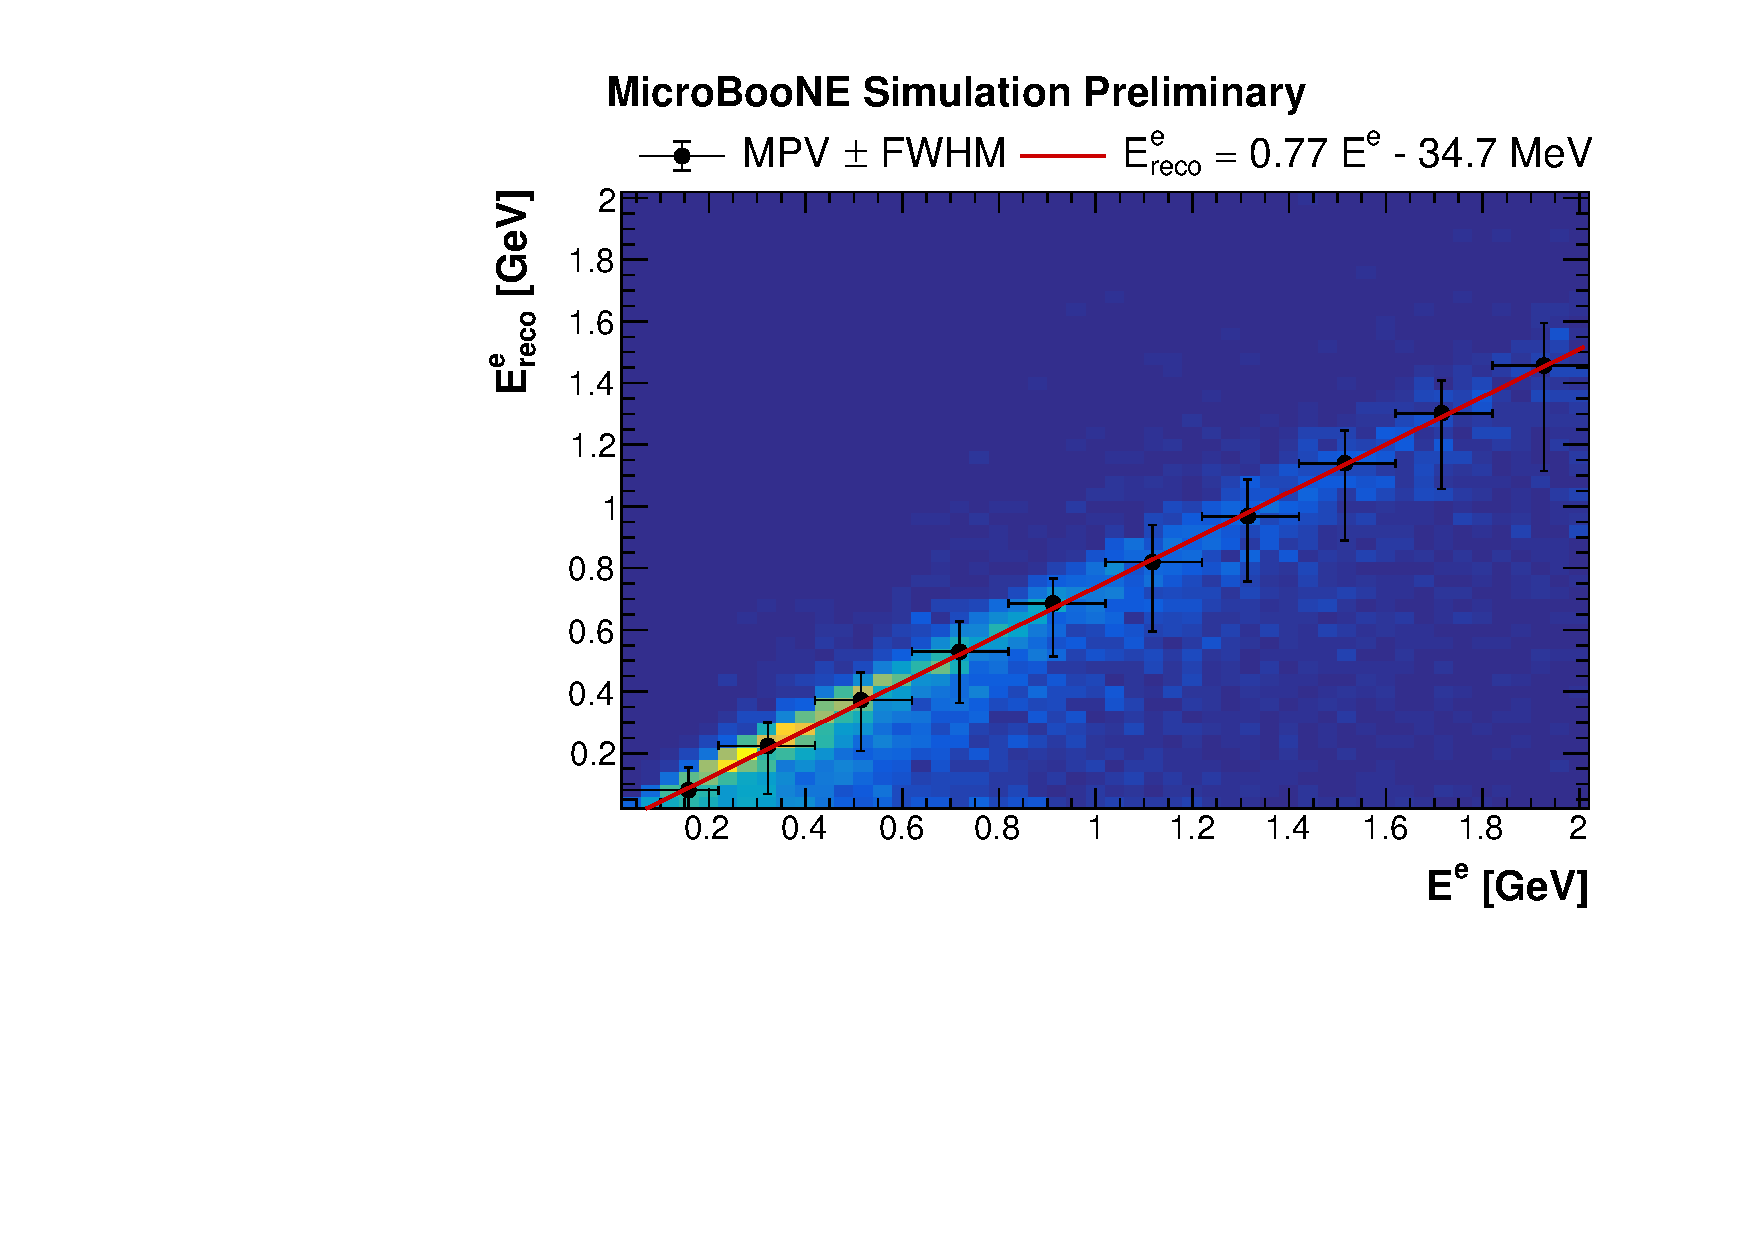
\includegraphics[width=0.65\columnwidth]{figures/ecalib.pdf}
\caption{Bi-dimensional histogram of true electron energy $E^{e}$ vs. reconstructed electron energy $E_{\mathrm{reco}}^{e}$. The reconstructed electron energy is measured summing the energy of each hit associated to reconstructed showers produced by the simulated electron. The black points correspond to the most probable value of the $E_{\mathrm{reco}}^{e}$ distribution for each $E^{e}$ bin, calculated with a GaussExp fit.}
\label{fig:ecalib}
\end{figure}

It is also possible to measure the energy resolution in the simulation by calculating the normalised difference $E_{\mathrm{frac}}$ between the corrected reconstructed energy $E^e_{\mathrm{corr}}$ and the true electron energy $E^e$:
\begin{equation}
    E_{\mathrm{frac}} = \frac{E^e_{\mathrm{corr}}-E^e}{E^e}.
\end{equation}
Figure \ref{fig:electron_res} shows the $E_{\mathrm{frac}}$ distribution for 10 intervals of equal size between 30 and 2030~MeV and the GaussExp fit for each distribution.

\begin{figure}[htbp]
\centering
\begin{overpic}[width=0.95\linewidth]{figures/electron_res.pdf}
\end{overpic}
% 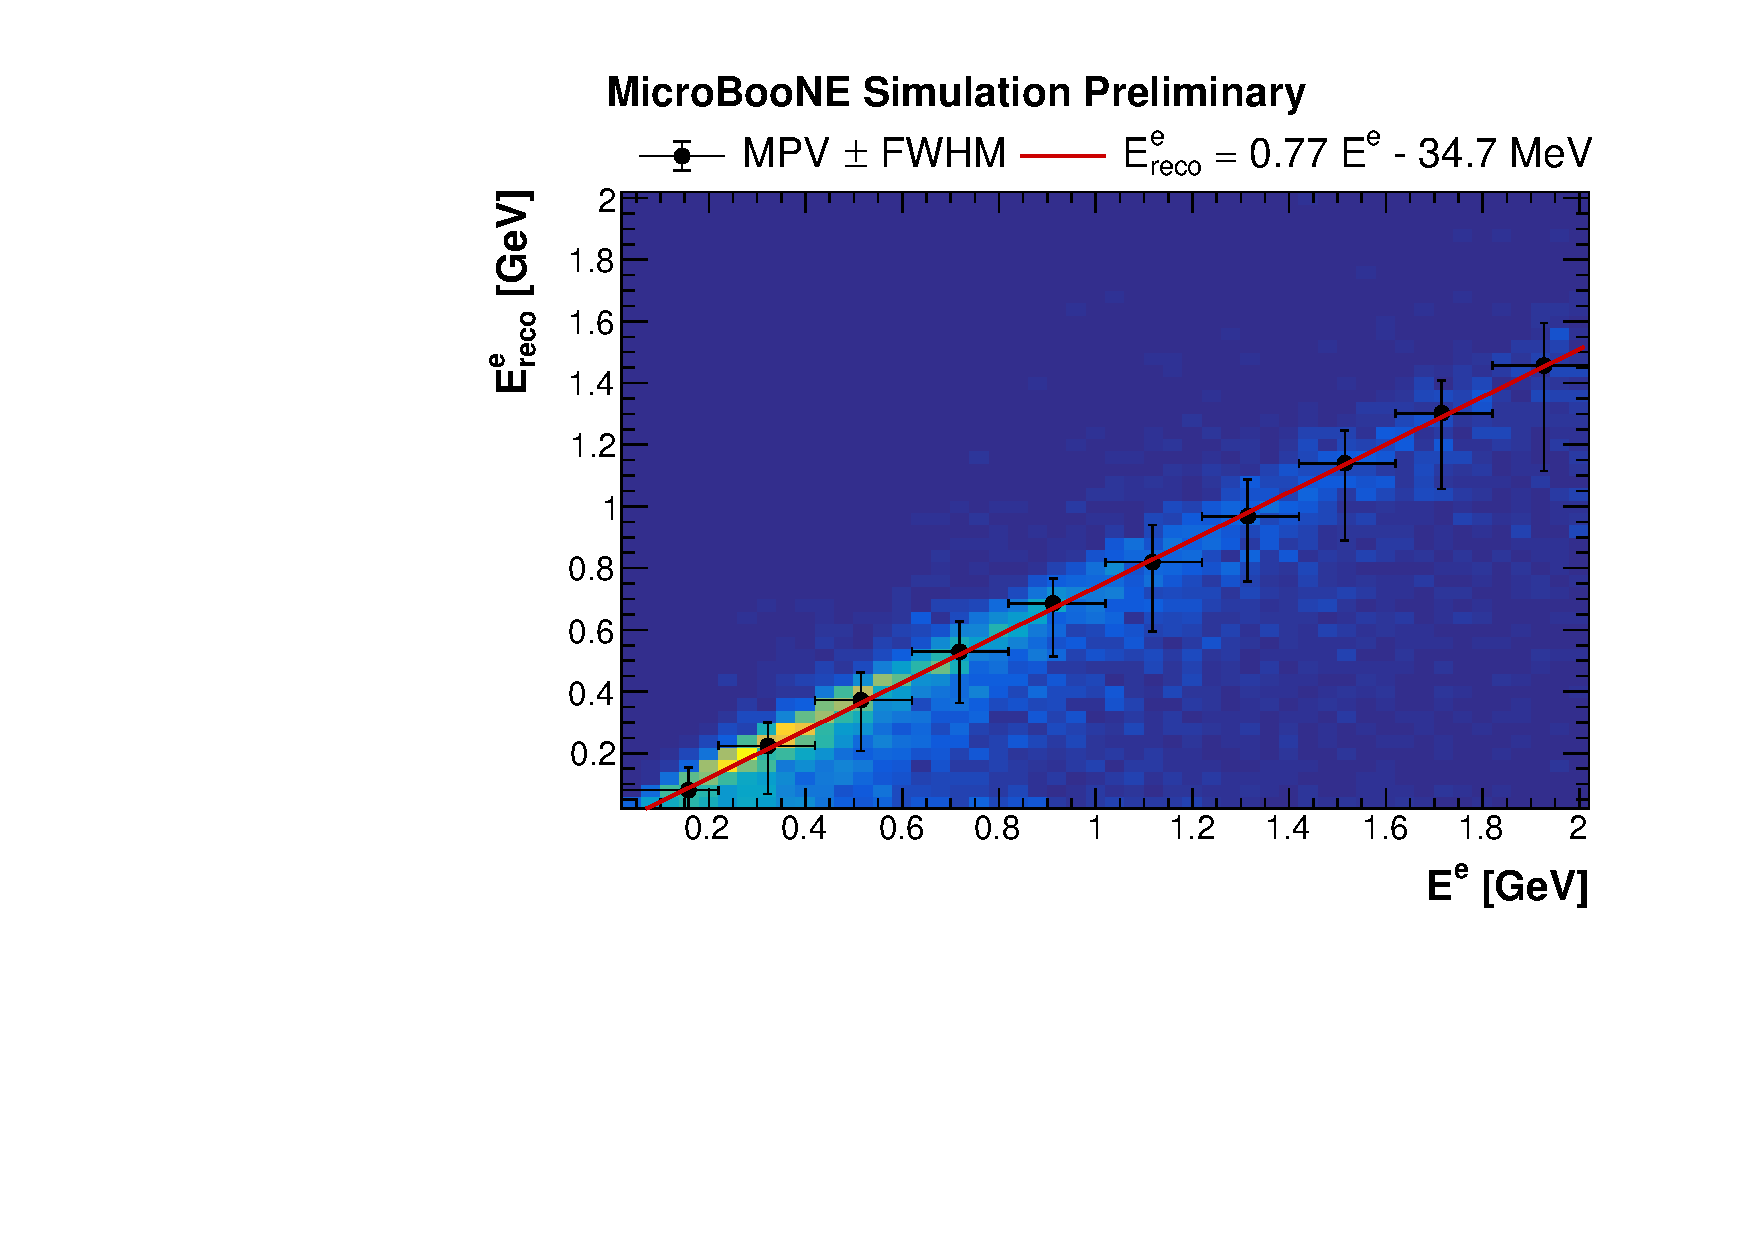
\includegraphics[width=0.65\columnwidth]{figures/ecalib.pdf}
\caption{Normalised energy difference $E_{\mathrm{frac}}$ for 10 intervals of equal size in the 30-2030 MeV energy range. The normalised energy difference distributions have been fitted with a GaussExp function (red line).}
\label{fig:electron_res}
\end{figure}

The fractional energy resolution can then be defined as the ratio between the standard deviation of the Gaussian core $\sigma$ of the GaussExp function and the true electron energy $E_e$. Figure \ref{fig:sigma_e} shows the fractional energy resolution as a function of the true electron energy. The points can be fitted with the classic calorimeter resolution formula \cite{Fabjan:2003aq}:
\begin{equation}
    \frac{\sigma}{E} = \frac{a}{\sqrt{E}} \oplus \frac{b}{E} \oplus c,\label{eq:calo}
\end{equation}
where:
\begin{itemize}
    \item $a = 2.30\%$ is the stochastic term, which is caused by the intrinsic fluctuations of the development of the electromagnetic shower;
    \item $b = 7.53\%$ is the noise term, which comes from the electronics noise of the readout chain and represents the dominant contribution;
    \item $c = 1.21\%$ is the constant term, which is caused by detector non-uniformities (e.g. the presence of missing or unresponsive wires).
\end{itemize} 

\begin{figure}[htbp]
\centering
\begin{overpic}[width=0.85\linewidth]{figures/sigma_e.pdf}
\end{overpic}
\caption{Fractional energy resolution for 10 intervals of equal size in the 30-2030 MeV energy range. The points have been fitted the classic calorimeter energy resolution formula \eqref{eq:calo}.}
\label{fig:sigma_e}
\end{figure}


Another effect which contributes to the broadening of the energy resolution in MicroBooNE is caused by wrong or sub-optimal clustering: if the pattern recognition fails to group together all the hits that corresponds to the electromagnetic shower, or if it includes hits belonging to ionisation tracks (e.g. from cosmic muons), the reconstructed energy will be respectively smaller or larger than the true electron energy.
It is also important to underline that the energy resolution quoted here does not correspond to the intrinsic MicroBooNE energy resolution, but only to the energy resolution for the selected $\nu_e$ CC0$\pi$-Np events.

\subsection{Single proton energy reconstruction and calibration}\label{sec:protonenergy}
Proton energy reconstruction is performed by converting the reconstructed track length $L$ into deposited energy using the proton stopping power in liquid argon tabulated in \cite{pstar}. Liquid argon density $\rho_{\mathrm{LAr}}$ is assumed to be constant at 1.4~g/ml. Figure \ref{fig:proton} shows the proton kinetic energy as a function of the range of the proton in liquid argon (measured as $L \times \rho_{\mathrm{LAr}}$).

\begin{figure}[htbp]
\centering
  \begin{subfigure}{0.49\textwidth}
  \begin{overpic}[width=\linewidth]{figures/proton.pdf}
\put(120,640){\tiny{\textsf{\textbf{MicroBooNE Simulation Preliminary}}}}
\end{overpic}
%     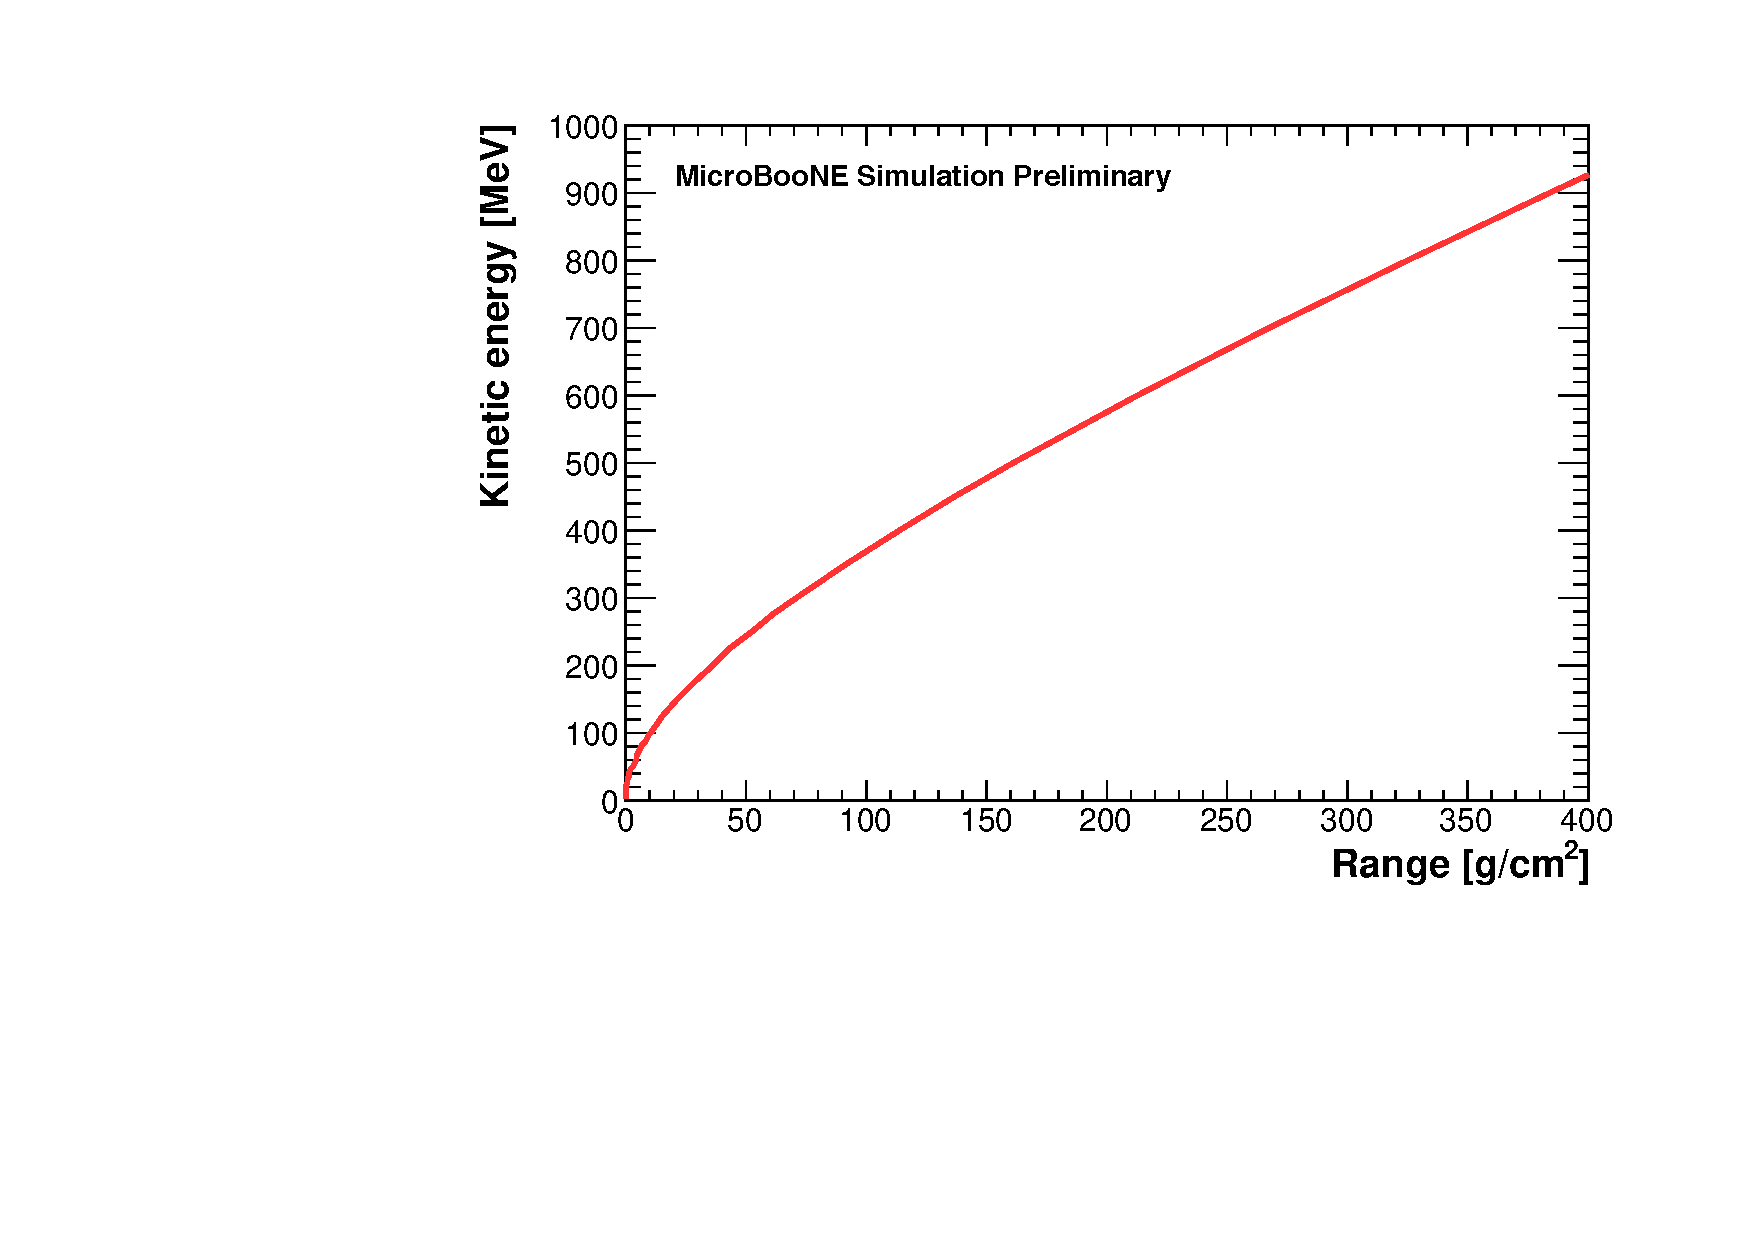
\includegraphics[width=\linewidth]{figures/proton.pdf}
    \caption{Proton kinetic energy as a function of the range of the proton in liquid argon.}\label{fig:proton}
  \end{subfigure}
  \begin{subfigure}{0.49\textwidth}
    \begin{overpic}[width=\linewidth]{figures/pcalib.pdf}\end{overpic}
% 	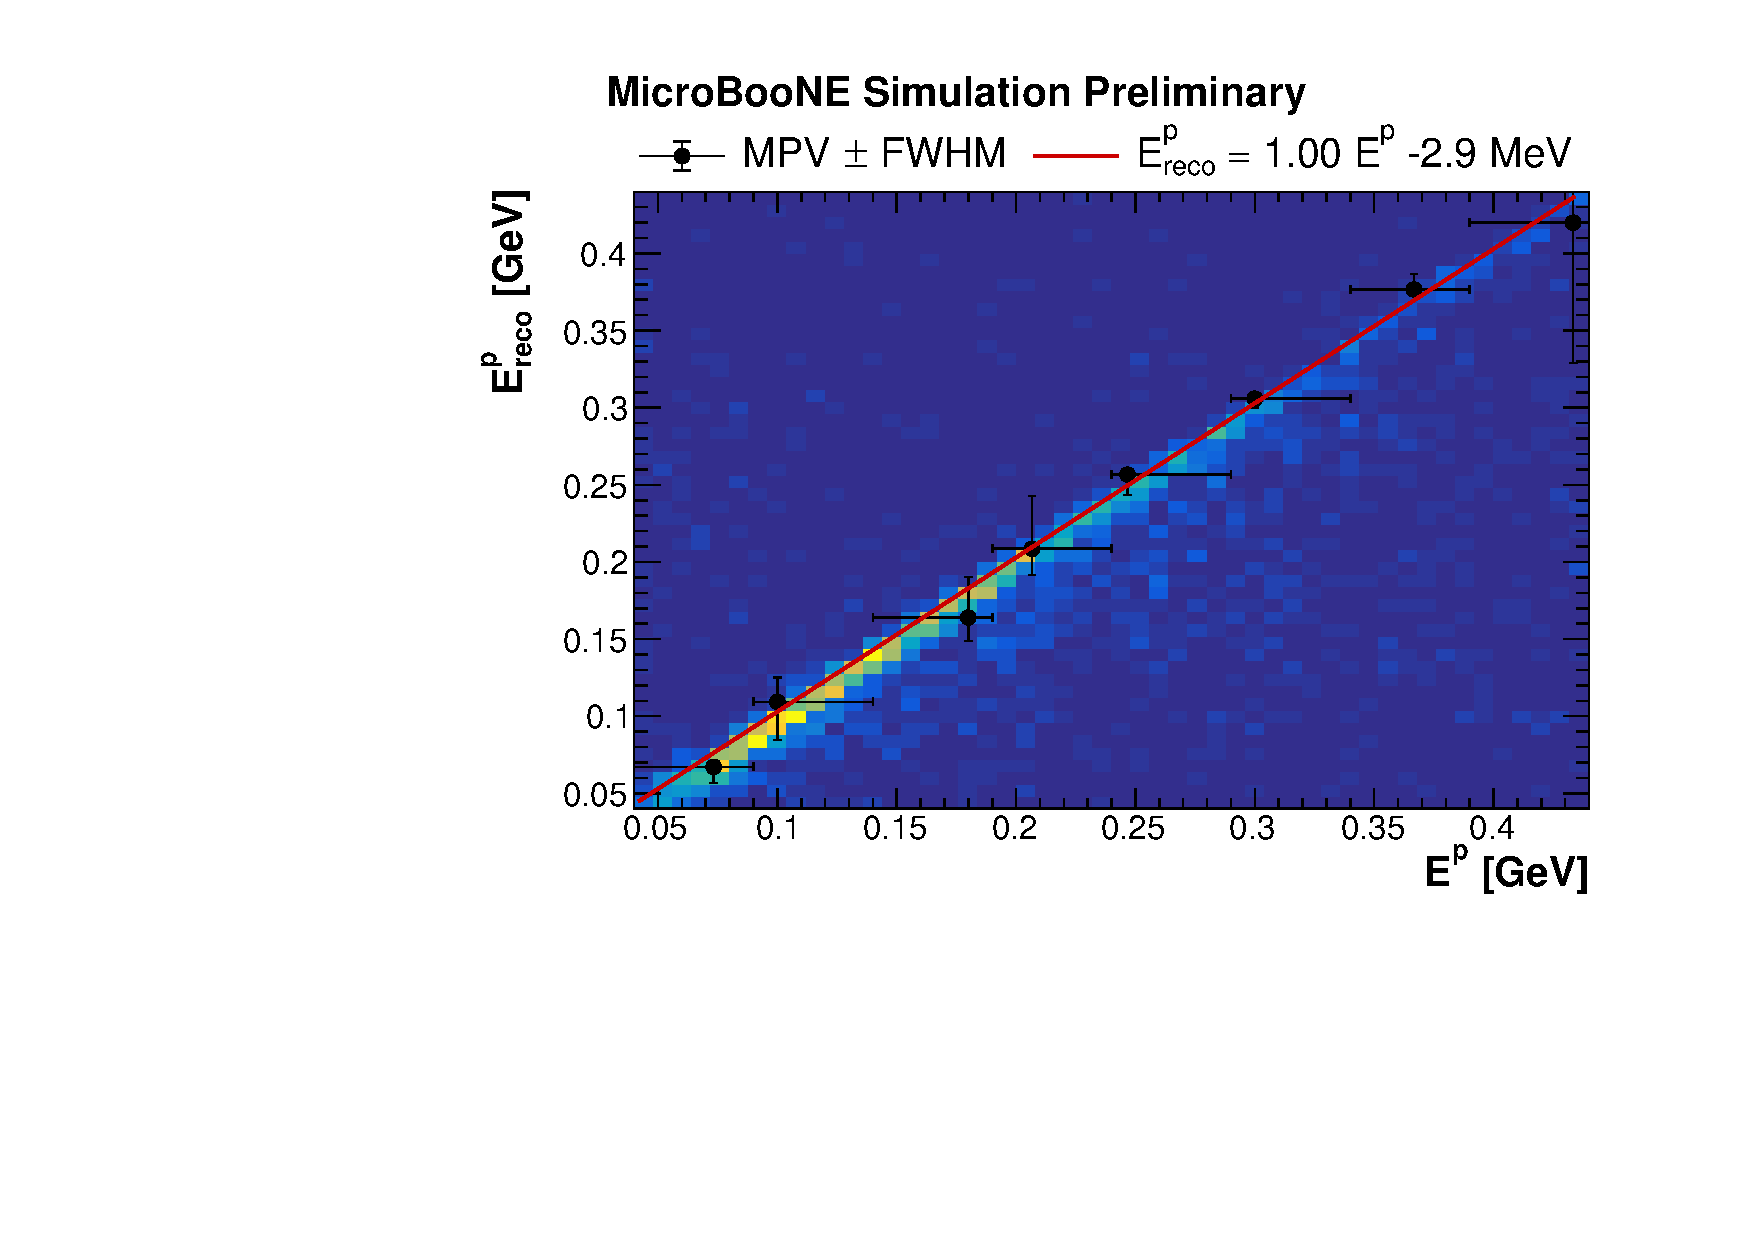
\includegraphics[width=\linewidth]{figures/pcalib.pdf}
     \caption{Bi-dimensional histogram of true proton energy $E^{p}$ vs. reconstructed proton energy $E_{\mathrm{reco}}^{p}$.}\label{fig:pcalib}
   \end{subfigure}
   \caption{The reconstructed proton energy is measured converting the reconstructed track length $L$ into deposited energy using the proton stopping power in liquid argon, as tabulated in \cite{pstar} (left). The calibration is calculated from a linear fit of the most probable values of the $E_{\mathrm{reco}}^{p}$ distribution for each $E^{p}$ bin (right).}
\end{figure}

The calibration constant has been obtained comparing the reconstructed energy of the proton with the true kinetic energy of the simulated proton, in a CC $\nu_{e}$ sample with only one proton in the final state. The true proton and the reconstructed tracks are required to be fully contained within the fiducial volume. Since protons are not minimum-ionising particles, in the case of two or more tracks (\emph{split tracks}) associated to the same proton, the reconstructed length of the tracks has been summed before calculating the corresponding kinetic energy.
Figure \ref{fig:pcalib} shows the calibration slope necessary to convert the proton reconstructed energy $E_{\mathrm{reco}}^{p}$ into true proton kinetic energy $E^{p}$. For each bin of the true proton energy, the most probable value of the corresponding proton reconstructed energy has been obtained with a GaussExp fit. A linear fit of the most probable values gives:
\begin{equation}
E_{\mathrm{reco}}^{p} = 1.00~E^{p} - 2.9~\mathrm{MeV}.
\end{equation}
The energy of the track, corrected by the calibration factor is then defined as:
\begin{equation}
E_{\mathrm{corr}}^{p} = (E_{\mathrm{reco}}^{p} + 2.9~\mathrm{MeV})/1.00
\end{equation}

\subsection{Deposited Energy Reconstruction}\label{sec:deposited}
It is possible to compare the total visible energy in the event $E_{\mathrm{k}}$, defined as the sum of the kinetic energies of the visible particles in the final state, with the sum of the reconstructed energies for shower-like ($E_{\mathrm{corr}}^{e}$) and track-like objects ($E_{\mathrm{corr}}^{p}$) for the selected $\nu_{e}$ CC0$\pi$-Np events. This quantity $E_{\mathrm{corr}}$ is defined as:
\begin{equation}
E_{\mathrm{corr}} = \sum^{N_{p}} E_{\mathrm{corr}}^{p} + \sum^{N_{e}} E_{\mathrm{corr}}^{e},
\end{equation}
where $N_{p}$ is the number of reconstructed tracks and $N_{e}$ is the number of reconstructed showers in the event. For events where we have two or more shower-like objects and no track-like objects, the shower-like object with the lowest proton $\chi^2$ score is chosen as proton candidate (see Section \ref{sec:proton_id}). In these cases we have $N_{p} = 1$ by definition.
The reconstructed energy does not include particles that do not interact in the liquid argon (such as neutrons) and charged particles with a kinetic energy below the detection threshold, defined in Section \ref{sec:eff}. Figure \ref{fig:nucalib} shows the calibration slope necessary to convert the the total reconstructed energy $E_{\mathrm{corr}}$ into visible energy $E_{\mathrm{k}}$. The plot has been obtained using the $\nu_{e}$ CC0$\pi$-Np + cosmic sample. A linear fit of the data points gives:
\begin{equation}
E_{\mathrm{k}} = 0.98~E_{\mathrm{corr}} - 28.5~\mathrm{MeV}.
\end{equation}
The reconstructed visible energy, corrected by the calibration factor is then defined as:
\begin{equation}
E_{\mathrm{deposited}} = (E_{\mathrm{corr}} + 28.5~\mathrm{MeV})/0.98
\end{equation}

Several effects can contribute to this calibration factor: among the others, the presence of regions with unresponsive of missing wires can cause an underestimation of the deposited energy. In the future, this effect can be limited by the use of the other two planes for calorimetric measurements.

\begin{figure}[htbp]
\centering
\begin{overpic}[width=0.85\linewidth]{figures/nucalib.pdf}
\end{overpic}\caption{Bi-dimensional histogram of total visible energy $E^{\mathrm{k}}$ vs. the total reconstructed energy $E_{\mathrm{corr}}$. Black points are obtained measuring the most probable value of the $E_{\mathrm{corr}}$ distribution for each $E_{\mathrm{k}}$ bin.} 
\label{fig:nucalib}
\end{figure}

In this analysis, we will use the quantity $E_{\mathrm{deposited}}$ as an estimate of the total visible energy in the event.

\subsection{Deposited energy binning}\label{sec:depositedenergy}
The binning of the deposited energy distribution must be carefully evaluated, since it is of fundamental importance in the calculation of the significance of an eventual excess. In this analysis, we require the events in a true $E_{\mathrm{k}}$ bin to fall in the same reconstructed $E_{\mathrm{deposited}}$ bin in at least 50\% of the cases for $\nu_e$~CC0$\pi$-Np events. A combination which satisfies this condition and maximises the number of bins in the $[0,3]$~GeV range is:
\begin{equation}
    E_{\mathrm{deposited}}\text{~bins} = [0, 0.2, 0.4, 0.6, 0.9, 1.25, 1.9, 3]~\text{GeV},
\end{equation}
which is then chosen as our binning for the $E_{\mathrm{deposited}}$ distributions.
Figure \ref{fig:migration} shows the migration matrix between $E_{\mathrm{deposited}}$ and $E_{\mathrm{k}}$. It shows the probability that an event with a true energy $E_{\mathrm{k}}$ in the $i$ bin has a reconstructed energy $E_{\mathrm{deposited}}$ in the same $i$ bin. Our binning criteria ensures that each element on the diagonal has a value larger than 0.50.

\begin{figure}[htbp]
\centering
\begin{overpic}[width=0.85\linewidth]{figures/migration.pdf}
\end{overpic}
\caption{Migration matrix between $E_{\mathrm{deposited}}$ and $E_{\mathrm{k}}$. It shows the probability that an event with a true energy $E_{\mathrm{k}}$ in the $i$ bin has a reconstructed energy $E_{\mathrm{deposited}}$ in the same $i$ bin.}
\label{fig:migration}
\end{figure}


\subsection{Measurement of the electromagnetic shower energy loss}\label{sec:dedx}
The mean energy loss per length of charged particles $\left\langle dE/dx\right\rangle$ can be described by the \emph{Bethe equation} as defined in Section 30.2.2 of \cite{PhysRevD.98.030001}:
\begin{equation}
    -\left\langle\frac{dE}{dx}\right\rangle = Kz^2\frac{Z}{A}\frac{1}{\beta^2}\left[\frac{1}{2}\ln\frac{2m_e c^2\beta^2\gamma^2 T_{\mathrm{max}}}{I^2}-\beta^2-\frac{\delta(\beta\gamma)}{2}\right],\label{eq:bethe}
\end{equation}
where $T_{\mathrm{max}}$ is the maximum possible energy transfer in a single collision, $I$ is the mean excitation energy, and $\delta(\beta\gamma)$ is a density correction. 

In materials of moderate thickness such as LAr, the energy loss probability distribution is described by the asymmetric Landau distribution \cite{Landau:1944if}, which drives the mean of the energy loss of eq. \eqref{eq:bethe} into the tail of the distribution. For this reason, ``the
mean of the energy loss given by the Bethe equation [\dots] is thus ill-defined
experimentally and is not useful for describing energy loss by single particles'' (Section 30.2.7 of \cite{PhysRevD.98.030001}).
The most probable value of the Landau distribution, which should be used instead, is given by: 
\begin{equation}
    \Delta_p = \xi\left[\ln\frac{2mc^2\beta^2\gamma^2}{I}+\ln\frac{\xi}{I}+j-\beta^2-\delta(\beta\gamma)\right],\label{eq:landau}
\end{equation}
where $\xi = (K/2)\langle Z/A \rangle (x/b^2)$~MeV, $j=0.2$, and $x$ is the thickness of the material in $\mathrm{g}\cdot\mathrm{cm}^2$ (Section 30.2.7 of \cite{PhysRevD.98.030001}). 

An important feature of the LArTPC technology is its ability to distinguish between electrons and photons in the final state by measuring their $dE/dx$. Photons that undergo pair-production, which is the dominant process above 10~MeV, produce a $e^+e^-$ pair. If the pair is boosted, the trajectories of the positron and the electron overlap, producing an average $dE/dx$ which is twice the one of a single, minimum-ionising electron. 

In MicroBooNE, the $dE/dx$ for electromagnetic showers is measured with a procedure analogous to the one developed by the ArgoNeuT collaboration and described in \cite{Acciarri:2016sli}. In this document, neutrinos were produced by the NuMI neutrino beam and the events were visually inspected to select electron and photon showers.

\begin{figure}[htbp]
\centering
\begin{overpic}[width=0.75\linewidth]{figures/evd_dedx.pdf}
\end{overpic}\caption{Event display of an electron shower candidate, showing the $1\times4$~cm$^2$ area used for the $dE/dx$ calculation. Each small black rectangle corresponds to a reconstructed shower hit.}
\label{fig:evd_dedx}
\end{figure}

In our implementation, as a first step, all the hits of the collection plane within a rectangle of 4~cm along the direction of the shower and 1~cm perpendicular to the shower are collected, as shown in the event display in Figure \ref{fig:evd_dedx}.

Subsequently, the $dQ/dx$ for each hit is measured dividing the collected charge ($dQ$) by the pitch ($dx$) between each hit and the next one along the shower direction. The pitch corresponds to the distance in the TPC that a particle travels between its two projections  on adjacent wires, which is \emph{at least} the wire spacing (3~mm for MicroBooNE \cite{Acciarri:2016smi}). Electromagnetic showers aligned with the wire direction correspond to a large value of the pitch. 

The $dE/dx$ is calculated from the $dQ/dx$ using the calibration factor measured in Section \ref{sec:showerenergy}, eq. \eqref{eq:calib}.
Since the Landau distribution of the $dE/dx$ hit values has an asymmetric tail, we assign to the shower the median (and not the mean) of the $dE/dx$ hit distribution, as an estimation the most probable value. The median metric has been proved in \cite{Acciarri:2016sli} to be to most robust over a variety of box lengths.

\begin{figure}[htbp]
\centering
\begin{overpic}[width=0.75\linewidth]{figures/dedx.pdf}
\end{overpic}\caption{Area-normalised distributions for the measured $dE/dx$ for simulated electrons and photons.}
\label{fig:dedx_gamma_e}
\end{figure}

Figure \ref{fig:dedx_gamma_e} shows the area-normalised histograms of the $dE/dx$ in the collection plane for simulated electron and photon showers. The events below 1~MeV/cm correspond for both distributions to showers with a low number of associated hits, or where the shower was mostly aligned with the wires of the collection plane (having as such a high pitch value). Figure \ref{fig:pitch} shows the pitch distribution in the collection plane and a bi-dimensional histogram of the $dE/dx$ vs. the pitch for photon showers: events with a $dE/dx$ below 1~MeV/cm mostly correspond to a high value of the pitch. 

\begin{figure}[htbp]
  \begin{subfigure}{0.49\textwidth}
  \begin{overpic}[width=0.88\linewidth]{figures/pitch.pdf}
\end{overpic}
    \caption{Pitch distribution for simulated electron showers in the collection plane (log-scale).}
  \end{subfigure}\hfill
  \begin{subfigure}{0.49\textwidth}
    \begin{overpic}[width=\linewidth]{figures/dedx_vs_pitch.pdf}\end{overpic}
     \caption{Bi-dimensional histogram of measured $dE/dx$ vs. pitch for photon showers.}
   \end{subfigure}
   \caption{Electromagnetic showers aligned with the wire orientation will have a large pitch value and their measured $dE/dx$ will be shifted towards low values.}\label{fig:pitch}
\end{figure}

The electron showers have a peak around 2~MeV/cm, as expected. The photon showers, instead, have a peak around 4~MeV/cm and a second peak around 2~MeV/cm, which represents a limitation to our $e/\gamma$ separation capabilities. This peak is caused by mainly two effects:
\begin{itemize}
    \item photons that undergo Compton scattering will transfer most of their energy to the electron, producing a shower with the same $dE/dx$ of an electron. This effect decreases with the photon energy and is dominant below 10~MeV, as shown in Figure \ref{fig:compton};
    
    \begin{figure}[htbp]
    \centering
    \begin{overpic}[width=0.75\linewidth]{figures/compton.png}
    \end{overpic}\caption{Cross section of gammas on argon between 1 MeV and 1 GeV. Here, $\kappa$ refers to the pair production cross section for the nuclear field and electron field. Compton scattering is dominant below 10 MeV. From \cite{Acciarri:2016sli}.}
    \label{fig:compton}
    \end{figure}
    
    \item very asymmetric $\gamma\rightarrow e^+e^-$ pair production. When the positron and the electron do not overlap, the measured $dE/dx$ distribution will be peaked around 2~MeV/cm. The electron and the positron can also be produced with very different energies, as shown in Figure \ref{fig:asymmetry}. In this case, the distribution of the $dE/dx$ values in the $1\times4$~cm$^2$ box will be shifted towards 2~MeV/cm. 
    
    \begin{figure}[htbp]
    \centering
    \begin{overpic}[width=0.75\linewidth]{figures/asymmetry.pdf}
    \end{overpic}\caption{Pair production relative cross-section as a function of the fraction of the photon energy $k$ transferred to either the electron or positron with energy $\epsilon$. From \cite{Caratelli:2018nob}.}
    \label{fig:asymmetry}
    \end{figure}
\end{itemize}

A comparison between the data and Monte Carlo distributions of the reconstructed showers $dE/dx$ is shown in Figure \ref{fig:dedx_datamc} of Section \ref{sec:bkg}.

\subsection{Particle identification of reconstructed tracks}\label{sec:proton_id}
The measurement of the $dE/dx$ along the reconstructed tracks allows to perform powerful particle identification, as demonstrated by a the ArgoNeuT collaboration in \cite{Acciarri:2013met}. 

This capability is particularly important for the search of low-energy electron neutrinos. A $\nu_e$ CC0$\pi$-1p neutrino interaction is topologically identical to a cosmic muon stopping in the LAr, since they both appear as a track with a small shower attached. However, the energy loss of a proton produced in a neutrino interaction is sensibly different from the one of a cosmic muon, for two main reasons:
\begin{itemize}
    \item the Bragg peak of the stopping cosmic muon corresponds to starting point of the Michel electron shower, while the Bragg peak of the proton track is far from the interaction vertex;
    \item the proton $dE/dx$ profile for protons differs from the $dE/dx$ profile for muons.
\end{itemize}
Being able to distinguish between proton and muon tracks is therefore essential in order to reject cosmogenic background. Events with a $\nu_{\mu}$ interaction with only a stopping muon in the final state can also be rejected with the same technique.

It is possible to parametrise the relation between the theoretical $dE/dx$ of a ionisation track and its \emph{residual range} with a power-law function:
\begin{equation}
    \frac{dE}{dx} = A R^b,
\end{equation}
where $A$, which has dimensions MeV/cm$^{1-b}$, and $b$, which is dimensionless, depend on the particle which produced the ionisation trail. The residual range $R$, in this case measured in centimetres, is the distance between a point on the track and its end ($R=0$ correspond to the track end-point).
Figure \ref{fig:range} shows the $dE/dx$ as a function of the residual range $R$ for several particle types. The values of $A$ and $b$ for each particle type are reported in Table \ref{tab:range}.

\begin{table}[htbp]
   \centering
   \caption{Stopping power parametrisation for various particle types in liquid argon (from \cite{Acciarri:2013met}.)}\label{tab:range}
   \begin{tabular}{lcr}
     \toprule
     Particle type & $A$ [MeV/cm$^{1-b}$] & $b$ \\
     \midrule
     Proton & 17 & -0.42 \\
     Kaon & 14 & -0.41 \\
     Pion & 8 & -0.37 \\
     Muon & 7 & -0.36 \\
     \bottomrule
   \end{tabular}
\end{table}

\begin{figure}[htbp]
\centering
\begin{overpic}[width=0.75\linewidth]{figures/range.pdf}
\end{overpic}\caption{Parametrised $dE/dx$ in liquid argon for various particles as a function of the residual range $R$. Parameters values can be found in Table \ref{tab:range}.}
\label{fig:range}
\end{figure}

The measured $dE/dx$ vs. $R$ profile can be compared with the theoretical expectation and the score of the $\chi^2$ test can be computed for different particle hypothesis. Figure \ref{fig:chi2} shows the $\chi^2$ score in the proton hypothesis for reconstructed proton tracks and reconstructed muon tracks in a Monte Carlo simulation. As expected, proton tracks are peaked at low values of the $\chi^2$, while the muon tracks correspond to much larger $\chi^2$ scores.

\begin{figure}[htbp]
\centering
\begin{overpic}[width=0.75\linewidth]{figures/chi2.pdf}
\end{overpic}\caption{Area-normalised distributions for the $\chi^2$ score in the proton hypothesis for reconstructed proton tracks and reconstructed muon tracks in a Monte Carlo simulation.}
\label{fig:chi2}
\end{figure}

A comparison between the data and Monte Carlo distributions of the $\chi^2$ score in the proton hypothesis is shown in Figure \ref{fig:proton_bkg} of Section \ref{sec:bkg}.

% Validation section should include: 
% Data/MC Agreement after precuts on all important variables
% Sideband Checks
% Corsika In-time vs BNB-ext
% Future Validation Studies

\section{Validation}
\subsection{Electromagnetic shower energy loss}
A way to verify if we are effectively selecting electron neutrinos is to study the distribution of the electromagnetic showers energy loss per length $dE/dx$. If the data events contain a well-reconstructed electron in the final state, the $dE/dx$ distribution will be peaked around 2~MeV/cm.
Figure \ref{fig:dedx_after} shows the $dE/dx$ distributions for data and Monte Carlo after the application of the rectangular cuts (left) and after the application of the BDTs cuts (right). As expected, the peak is in both cases around 2~MeV/cm, meaning that the $dE/dx$ of the reconstructed showers in data are compatible with electrons in the final state.

\begin{figure}[htbp]
\centering
  \begin{subfigure}{0.48\textwidth}
    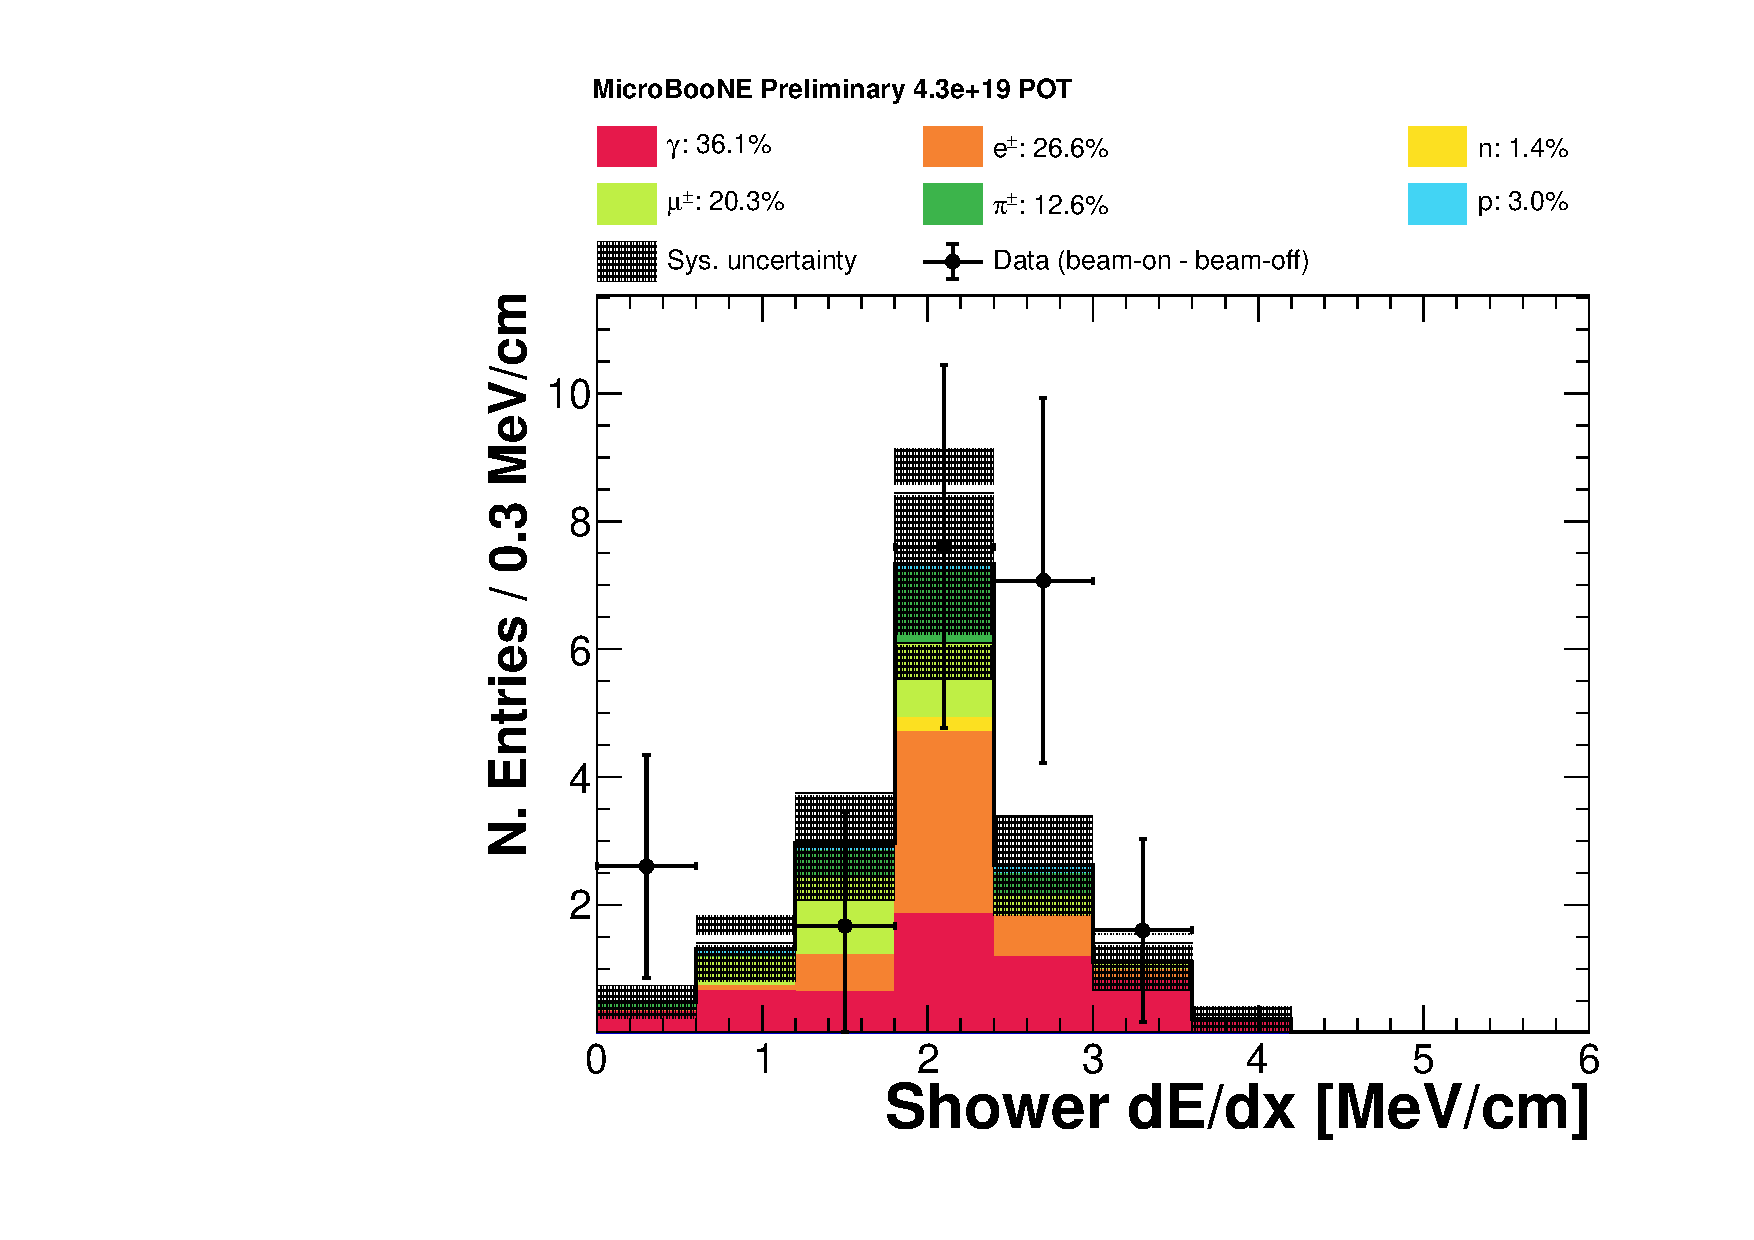
\includegraphics[width=\linewidth]{figures/dedx_cuts.pdf}
    \caption{Rectangular cuts.} 
  \end{subfigure}
    \begin{subfigure}{0.48\textwidth}
    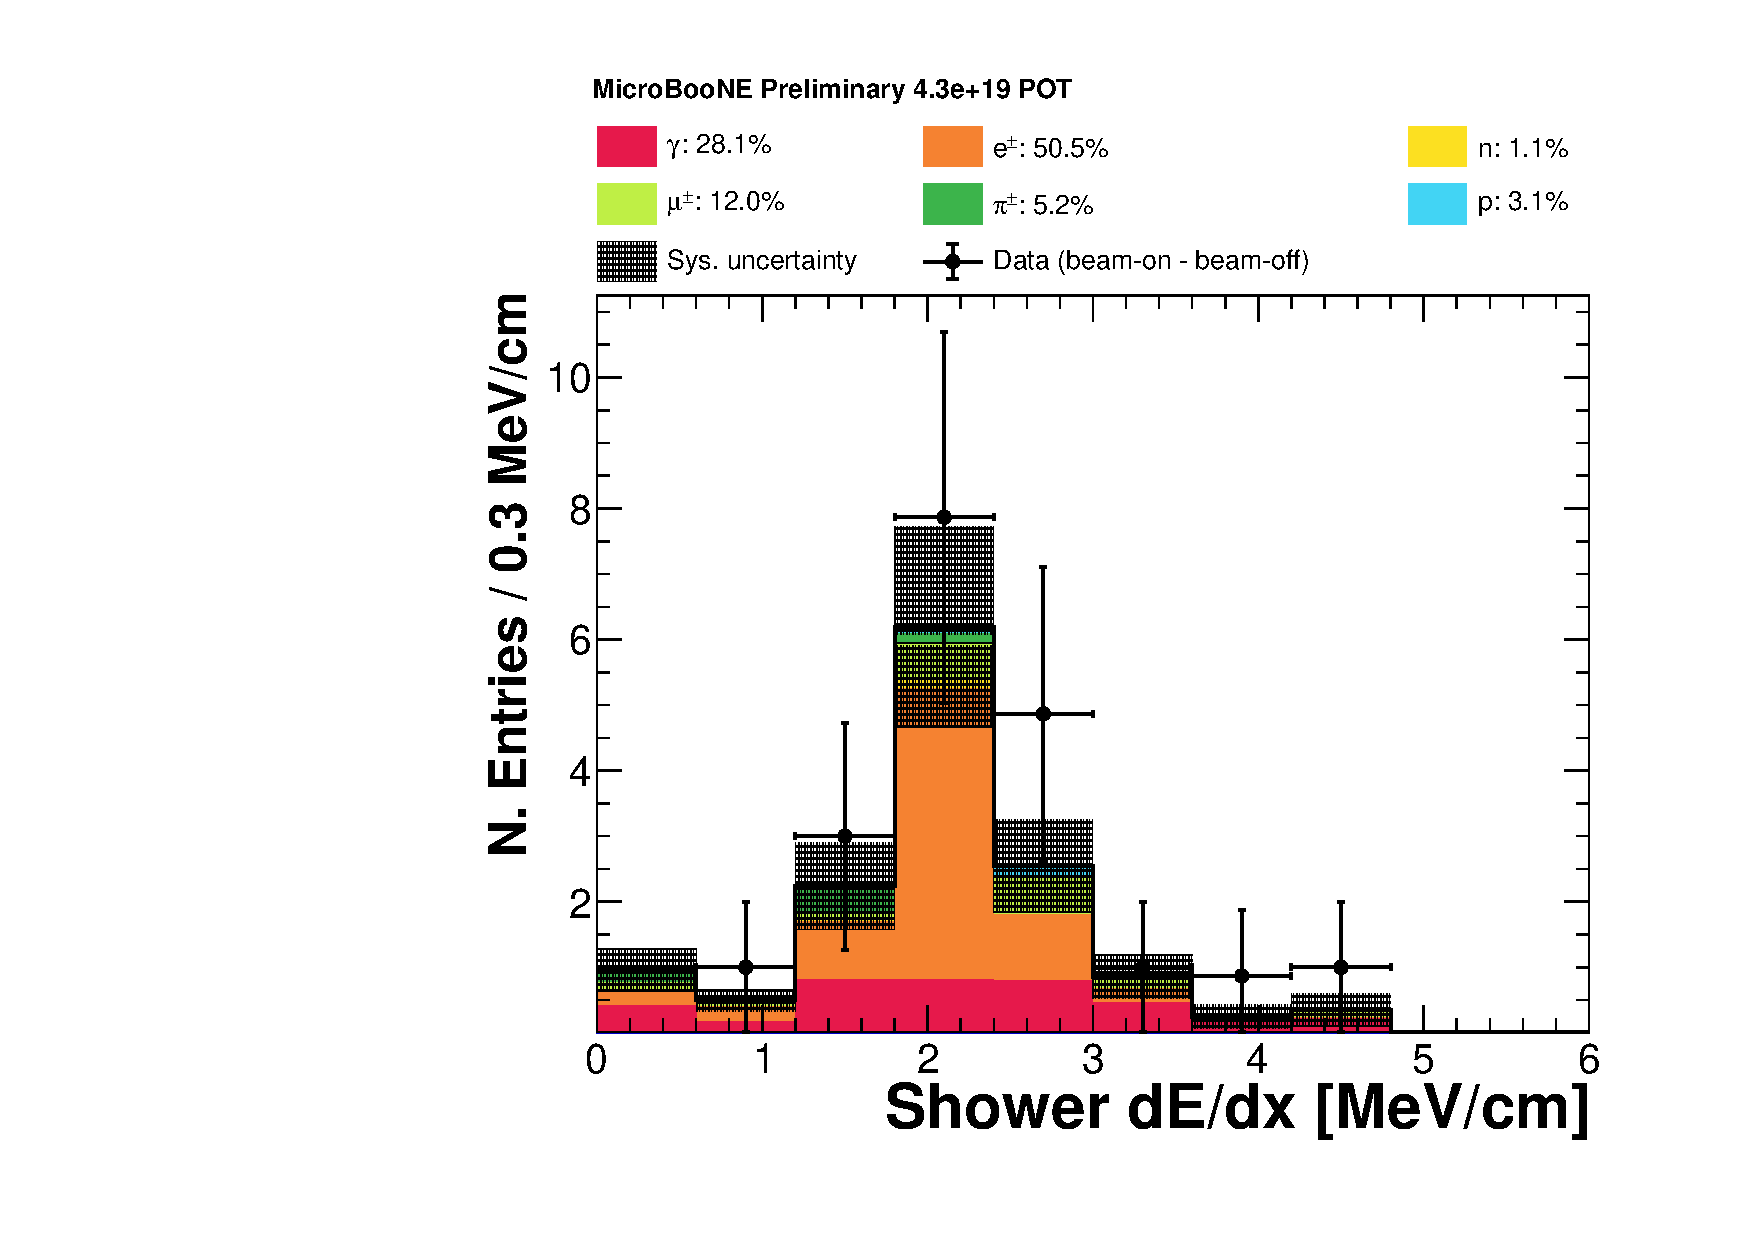
\includegraphics[width=\linewidth]{figures/dedx_bdt.pdf}
    \caption{BDTs.} 
  \end{subfigure}
  \caption{Distribution of the reconstructed showers $dE/dx$ after rectangular cuts (left) and BDTs cuts (right). The black points represent the statistical subtraction of the data beam-off events from the data beam-on events. The coloured stacked histograms represent the simulated events, classified according to the particle which generated the shower.}
  \label{fig:dedx_after}
\end{figure}

\subsection{Side-bands checks}
In this section we will study the agreement between data and Monte Carlo for selected samples orthogonal to the $\nu_{e}$ CC0$\pi$-Np-enriched sample obtained in Section \ref{sec:bkg}. In order to validate the analysis, some of the background-rejecting cuts are inverted or removed in order to enhance different background components.
\subsubsection{NC-enhanced selection}
It is possible to enhance the neutral-current component (defined as \emph{beam intrinsic NC} in our analysis) by (1) inverting the cut on the shower $dE/dx$, and (2) removing the cut on the shower distance (see Figures \ref{fig:dedx_norm}, \ref{fig:showerd_norm}). The $dE/dx$ of the most energetic shower must be within 3.2~MeV/cm and 5~MeV/cm to select electromagnetic cascades that were initiated by a photon. It also ensures that this NC-enhanced sample is orthogonal to the $\nu_{e}$ CC0$\pi$-Np selected sample. The cut on the shower distance is removed to include events where the photon conversion is far from the neutrino interaction vertex.
Thus, our final sample will mainly contain NC events, with some contamination of $\nu_{\mu}$ CC$\pi^{0}$ events where the muon track was tagged as a proton-like track.

\begin{figure}[htbp]
\centering
  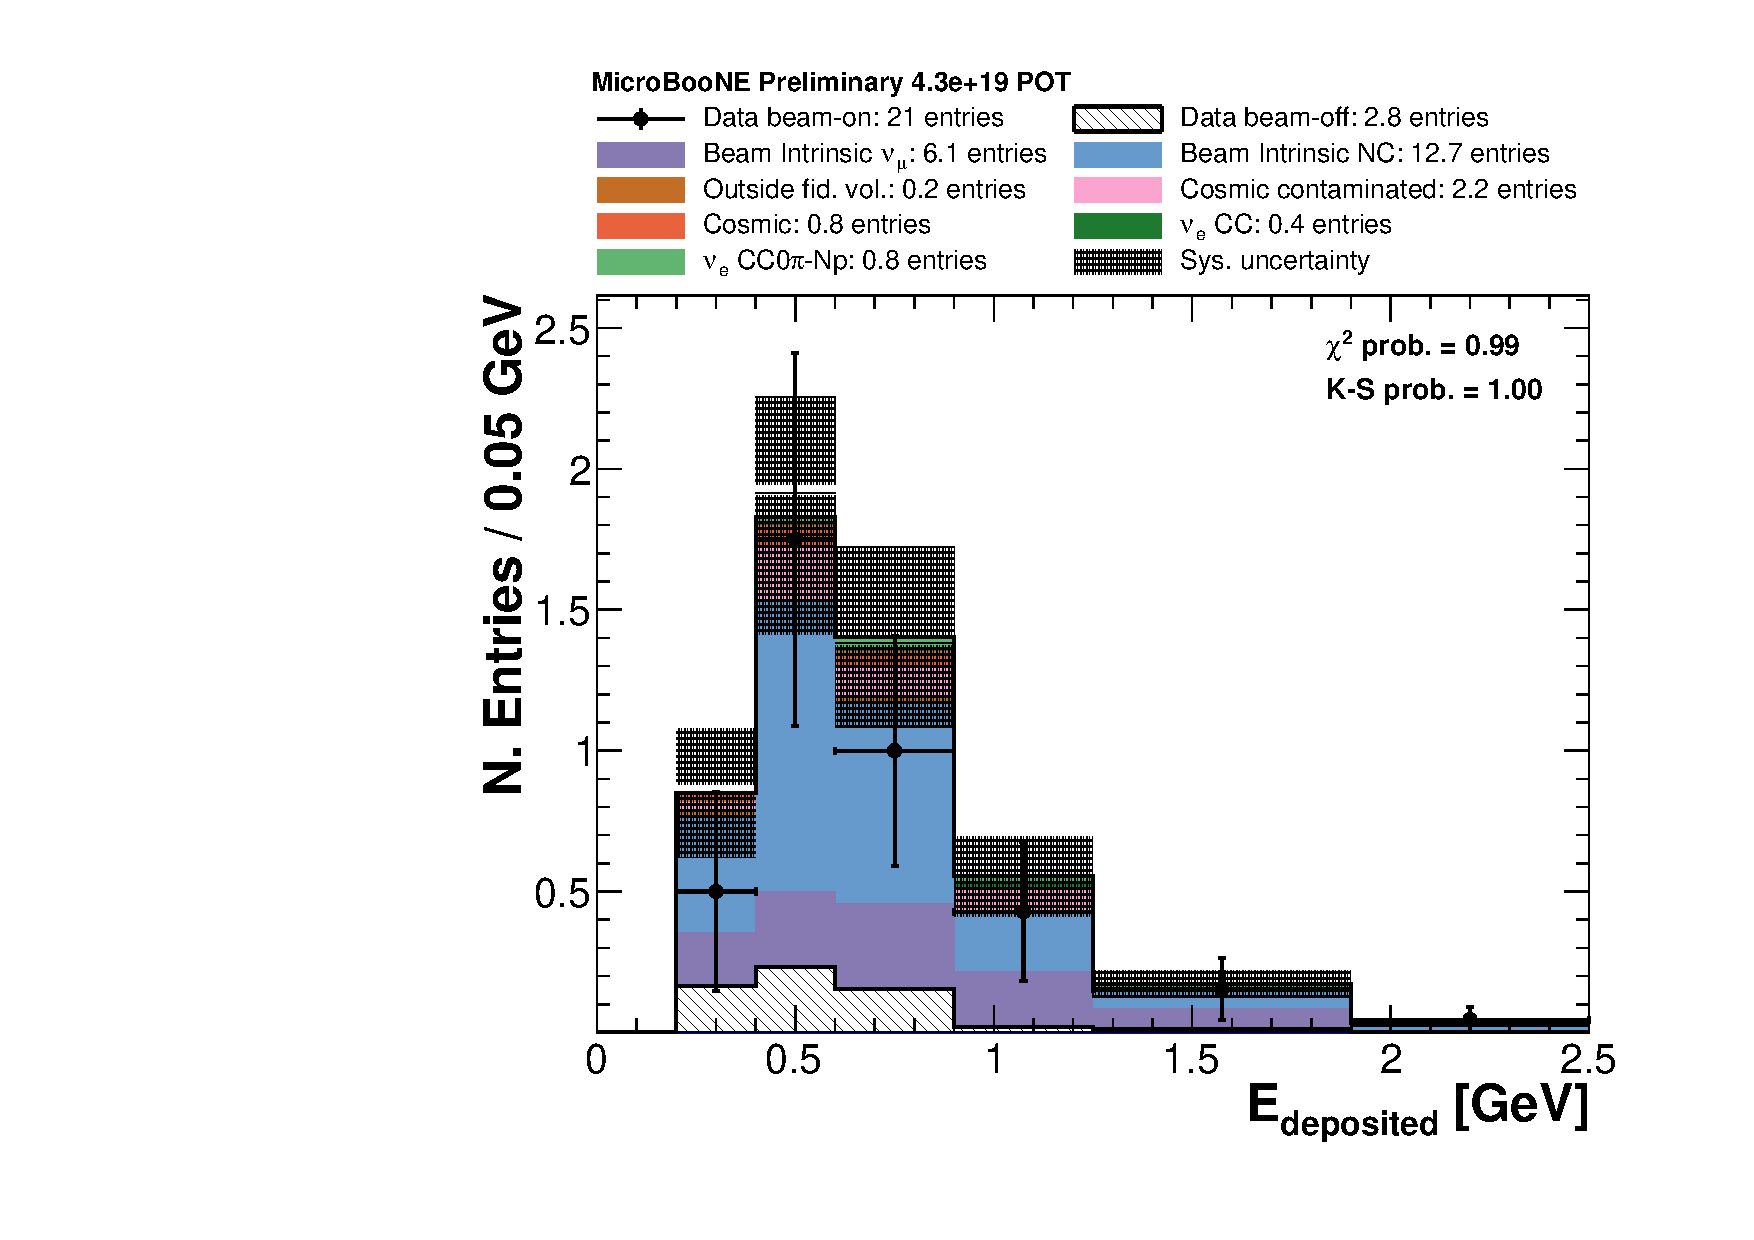
\includegraphics[width=0.7\linewidth]{figures/nc_reco.pdf}
  \caption{Reconstructed energy spectrum of the events selected with the NC-enhanced reverse cuts. The black points represent the data with statistical uncertainties. The coloured stacked histograms represent the simulated events, with the hatched histogram corresponding to the data beam-off sample. The shaded area represents the systematic uncertainty.}\label{fig:photon}
\end{figure}

Figure \ref{fig:photon} shows the comparison between data and Monte Carlo for the reconstructed energy spectrum $E_{deposited}$ of the NC-enhanced event spectrum. The agreement is good both in shape and normalisation: the data points are within the systematic uncertainties of the simulation in every bin.
%The reconstructed energy $E_{corr}$ here corresponds to the sum of the reconstructed energies of the shower-like objects and the reconstructed energies of the track-like objects $E_{corr} = E_{corr}^{p}+E_{corr}^{e}$.



\subsubsection{CC \texorpdfstring{$\nu_{\mu}$}{numu}-enhanced selection}
It is possible to enhance the presence of the CC $\nu_{\mu}$ background (defined as \emph{beam intrinsic $\nu_{\mu}$} in our analysis) by (1) removing the cut on the total number of hits in the collection plane, (2) removing the cut on the fraction of shower hits, (3) requiring a minimum track length, (4) requiring at least a track with $40 < \chi_p^{2} < 220$ (muon-like track), and (5) requiring that the event is selected by the external $\nu_{\mu}$ CC-inclusive analysis \cite{ubxsec} (see Figures \ref{fig:nhits_integral}, \ref{fig:ratio_norm}, \ref{fig:length_norm}, and \ref{fig:proton_norm}). Also in this case the CC $\nu_{\mu}$-enhanced sample will be orthogonal to the $\nu_{e}$ CC0$\pi$-Np selected sample.
A CC $\nu_{\mu}$ event has, by definition, a muon in the final state: as such, requiring a track length larger than 20~cm and changing the cut on the proton $\chi^2_p$ score decreases our muon-rejection power. The goal of the external analysis is to select CC $\nu_{\mu}$ events, so instead of vetoing those events as described in Section \ref{sec:numu}, we invert this requirement by allowing only these events.

\begin{figure}[htbp]
\centering
  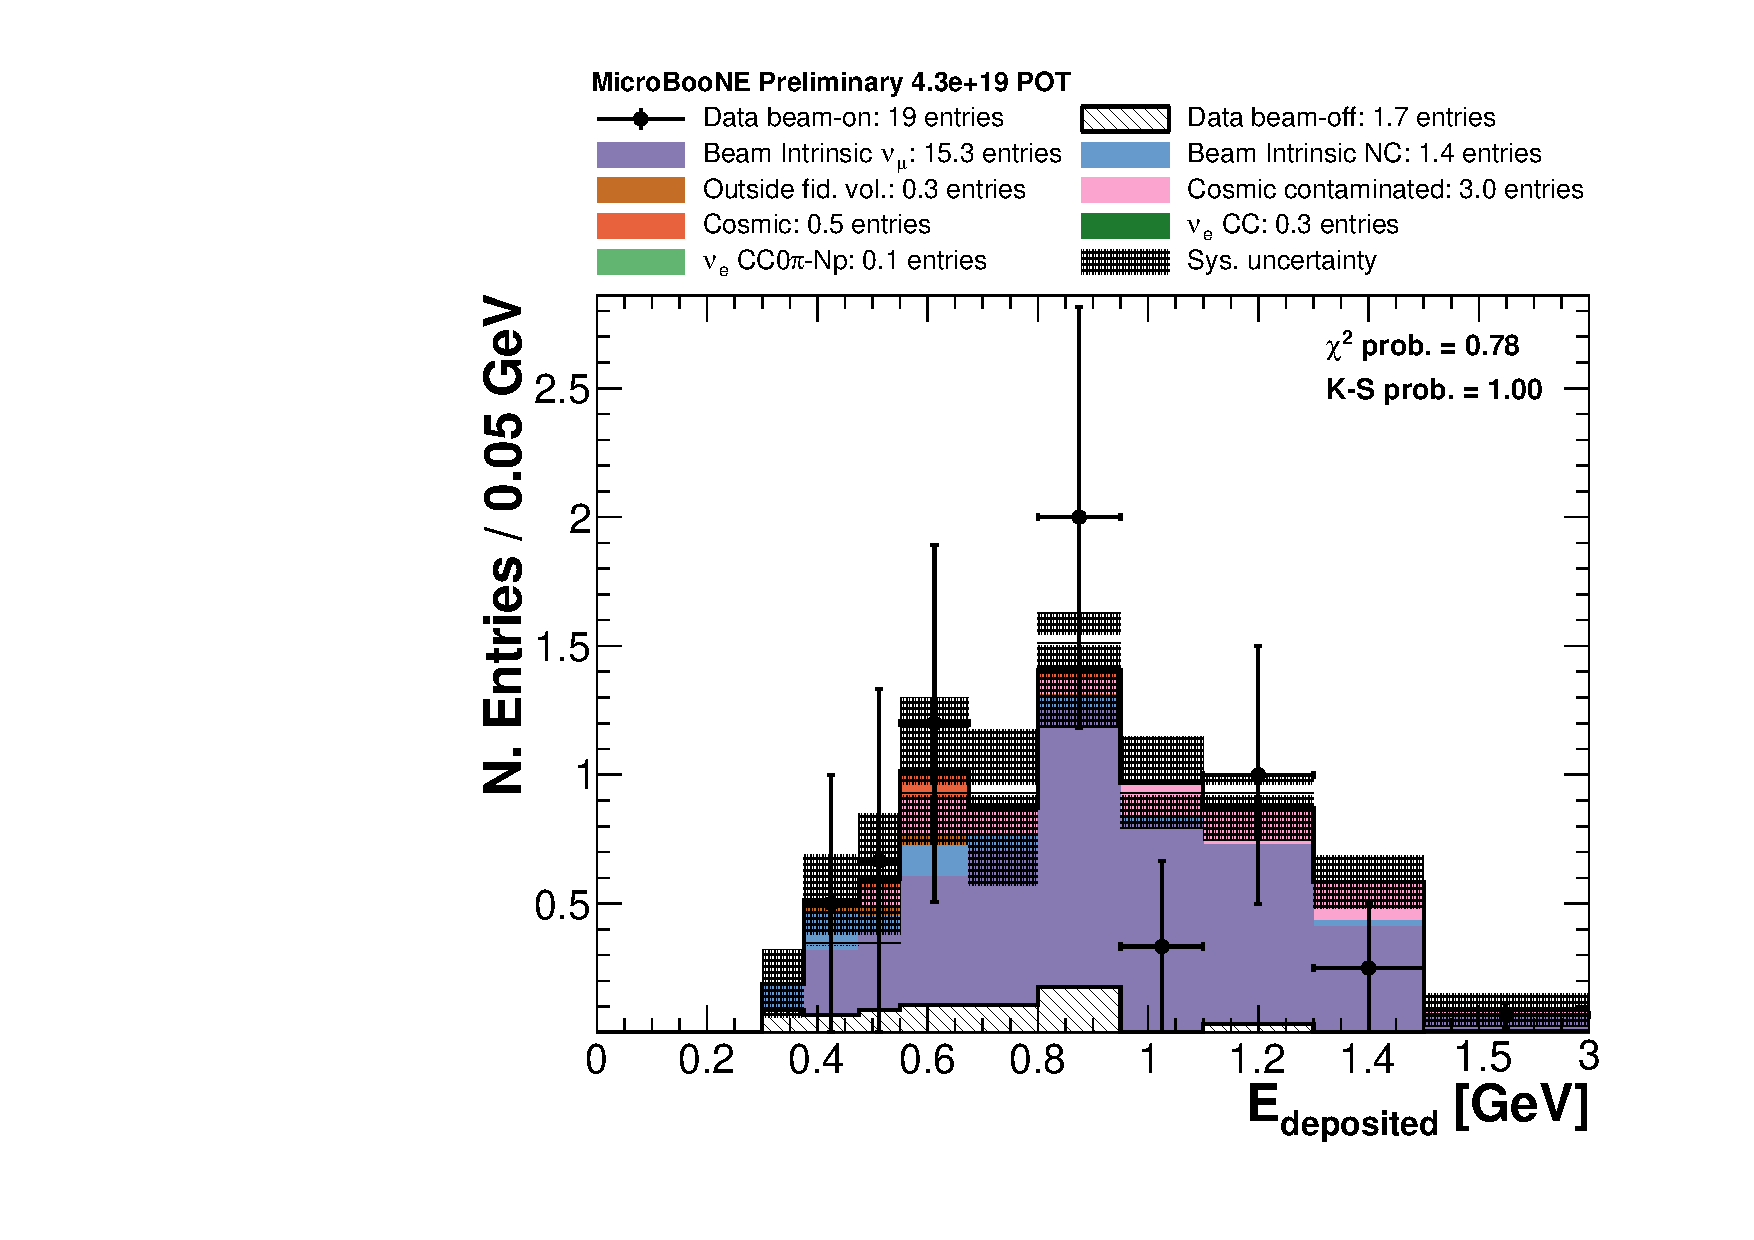
\includegraphics[width=0.7\linewidth]{figures/numu_reco.pdf}
  \caption{Reconstructed energy spectrum of the events selected with the CC~$\nu_{\mu}$-enhanced reverse cuts. The black points represent the data with statistical uncertainties. The coloured stacked histograms represent the simulated events, with the hatched histogram corresponding to the data beam-off sample. The shaded area represents the systematic uncertainty. The bottom part of the plot shows the ratio between the data beam-on events and the stacked histograms.}\label{fig:numu_inverted}
\end{figure}

Figure \ref{fig:numu_inverted} shows the agreement between data and Monte Carlo for the reconstructed energy spectrum of the CC $\nu_{\mu}$-enhanced event sample.
The agreement is good both in shape and normalisation: the data points are within the systematic uncertainties of the simulation in every bin.



% \subsection{Future Validation Studies}

% \subsubsection{Cosmic-ray studies}
% In order to validate the cosmic-ray components of our selected events it is possible to compare simulated events with a CORSIKA cosmic ray producing a flash in the optical system during the beam-gate window and the data off-beam sample. 
% In this way we will be able to check if the distributions of the variables we use (e.g. shower energy, shower $dE/dx$) show a good agreement between the simulation and a well-understood set of data events. 
% It will help to validate the cosmic background components and also the energy and $dE/dx$ reconstruction procedures.

\subsection{NuMI beam event studies}
It is possible to run this analysis on the complementary and independent neutrino dataset, acquired with the NuMI beam trigger. The NuMI beam is created from 120 GeV protons hitting a carbon target \cite{Adamson:2015dkw}, while the BNB is created from 8 GeV protons on a beryllium target. The NuMI beam has also a higher intrinsic $\nu_{e}$ component than the BNB (5\% vs. 0.5\%). Figure \ref{fig:numibeam} shows a comparison of the NuMI and BNB beam fluxes for the MicroBooNE detector. Even though it is around $8^{\circ}$ off-axis, MicroBooNE still receives $\sim2500$ $\nu_{e}$ interactions per year. 

As such, a study of the events selected in the NuMI dataset is of fundamental importance to validate the $\nu_{e}$ CC0$\pi$-Np selection algorithm, since it provides a completely independent set of electron neutrinos with different energy and angular distributions. 
However, the price to pay is the poor understanding of the flux at such off-axis angle. This does not affect the validation, but it makes a search for an excess extremely challenging. 

\begin{figure}[htbp]
\centering
  \begin{subfigure}{0.45\textwidth}
    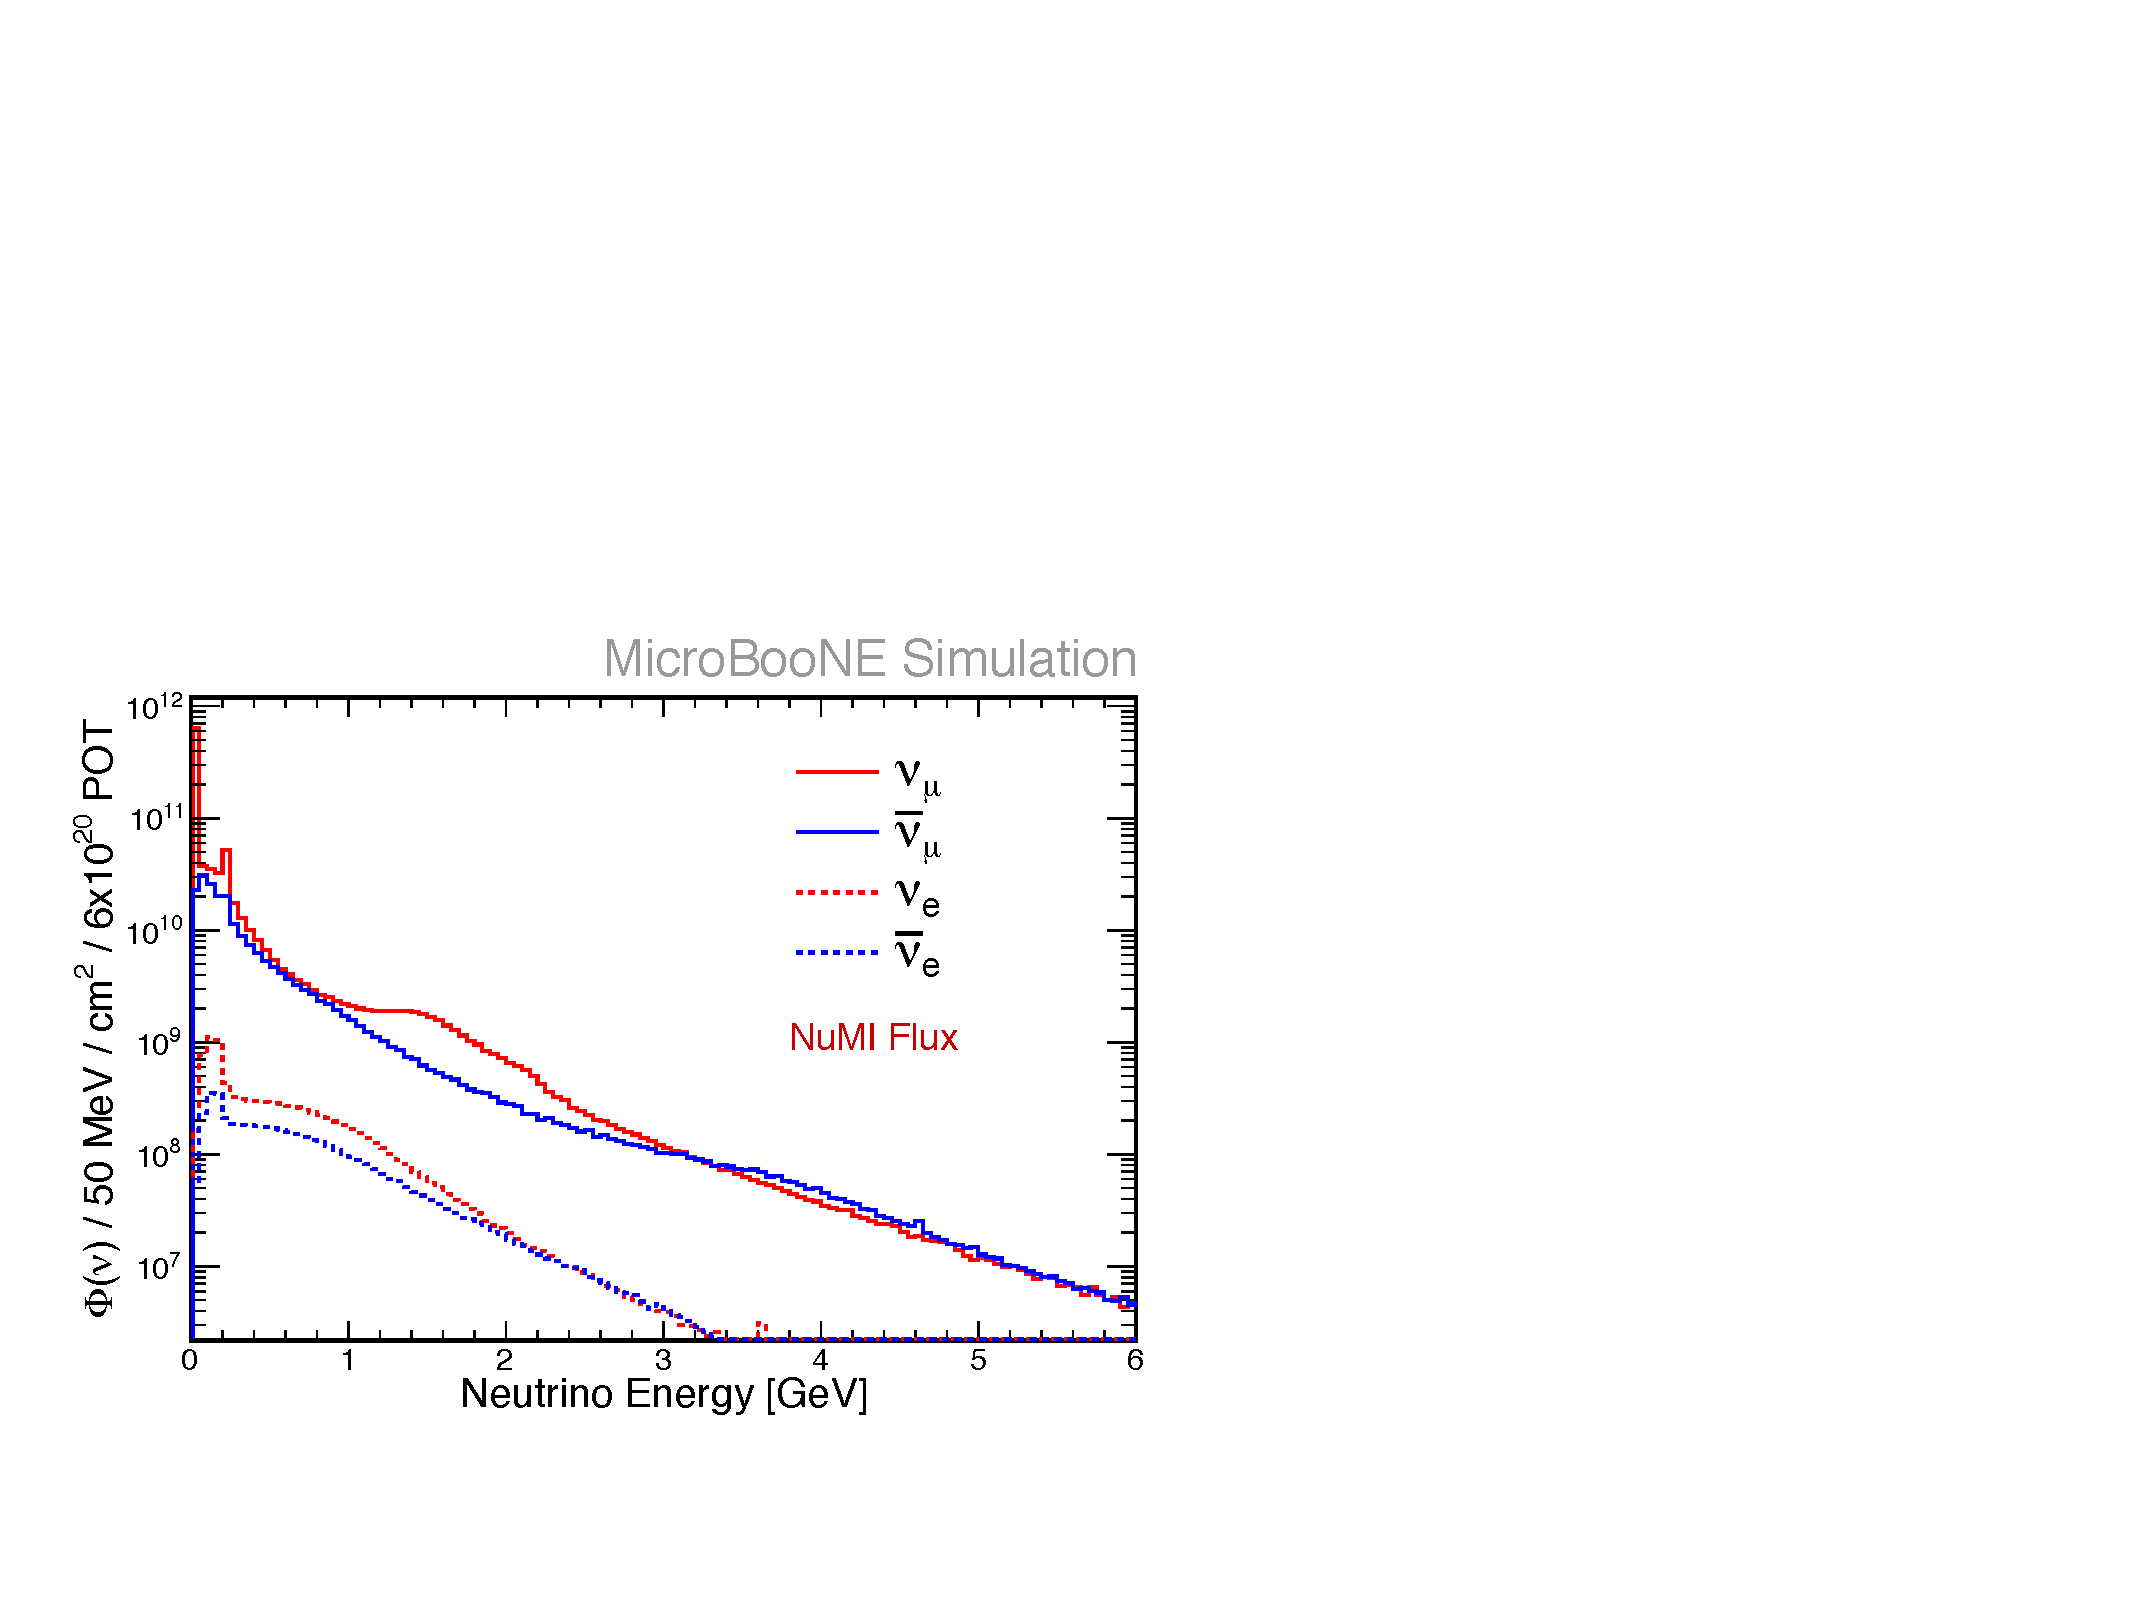
\includegraphics[width=\linewidth]{figures/numi.pdf}
    \caption{NuMI beam flux.} 
  \end{subfigure}
    \begin{subfigure}{0.45\textwidth}
    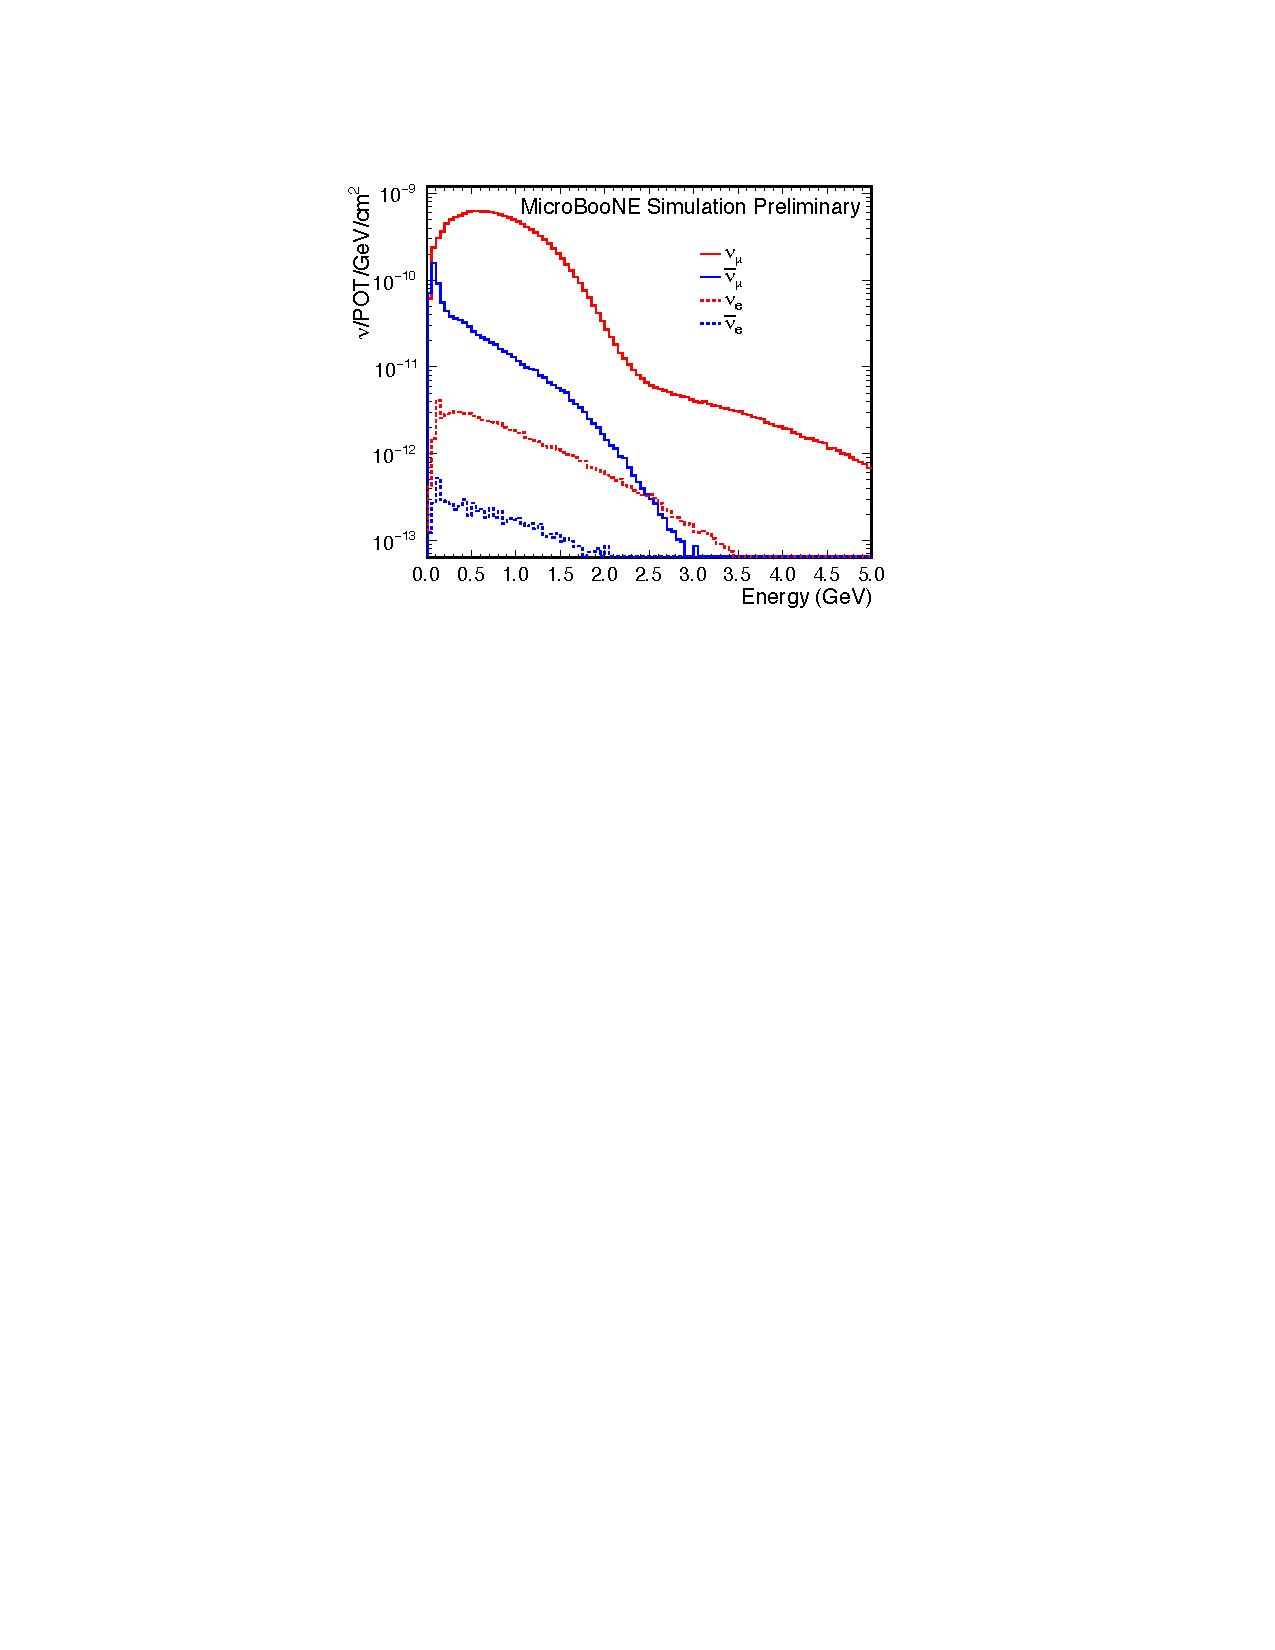
\includegraphics[width=\linewidth]{figures/bnbflux.pdf}
    \caption{BNB beam flux.} 
  \end{subfigure}
  \caption{NuMI and BNB neutrino fluxes for each neutrino and antineutrino component, when the beams are in neutrino mode.}\label{fig:numibeam}
\end{figure}

In order to run on this data sample, it is necessary to change the requirement on the reconstructed flash, since the beam-gate window is $[6,16]$~\si{\micro}s after the trigger time.
We apply the same rectangular cuts described in Section \ref{sec:cuts}, plus a threshold of 100~MeV on the reconstructed energy of the leading shower. This last cut allows us to remove a large fraction of cosmogenic background without significantly affecting our $\nu_e$ CC0$\pi$-Np selection efficiency.

\begin{figure}[htbp]
\centering
  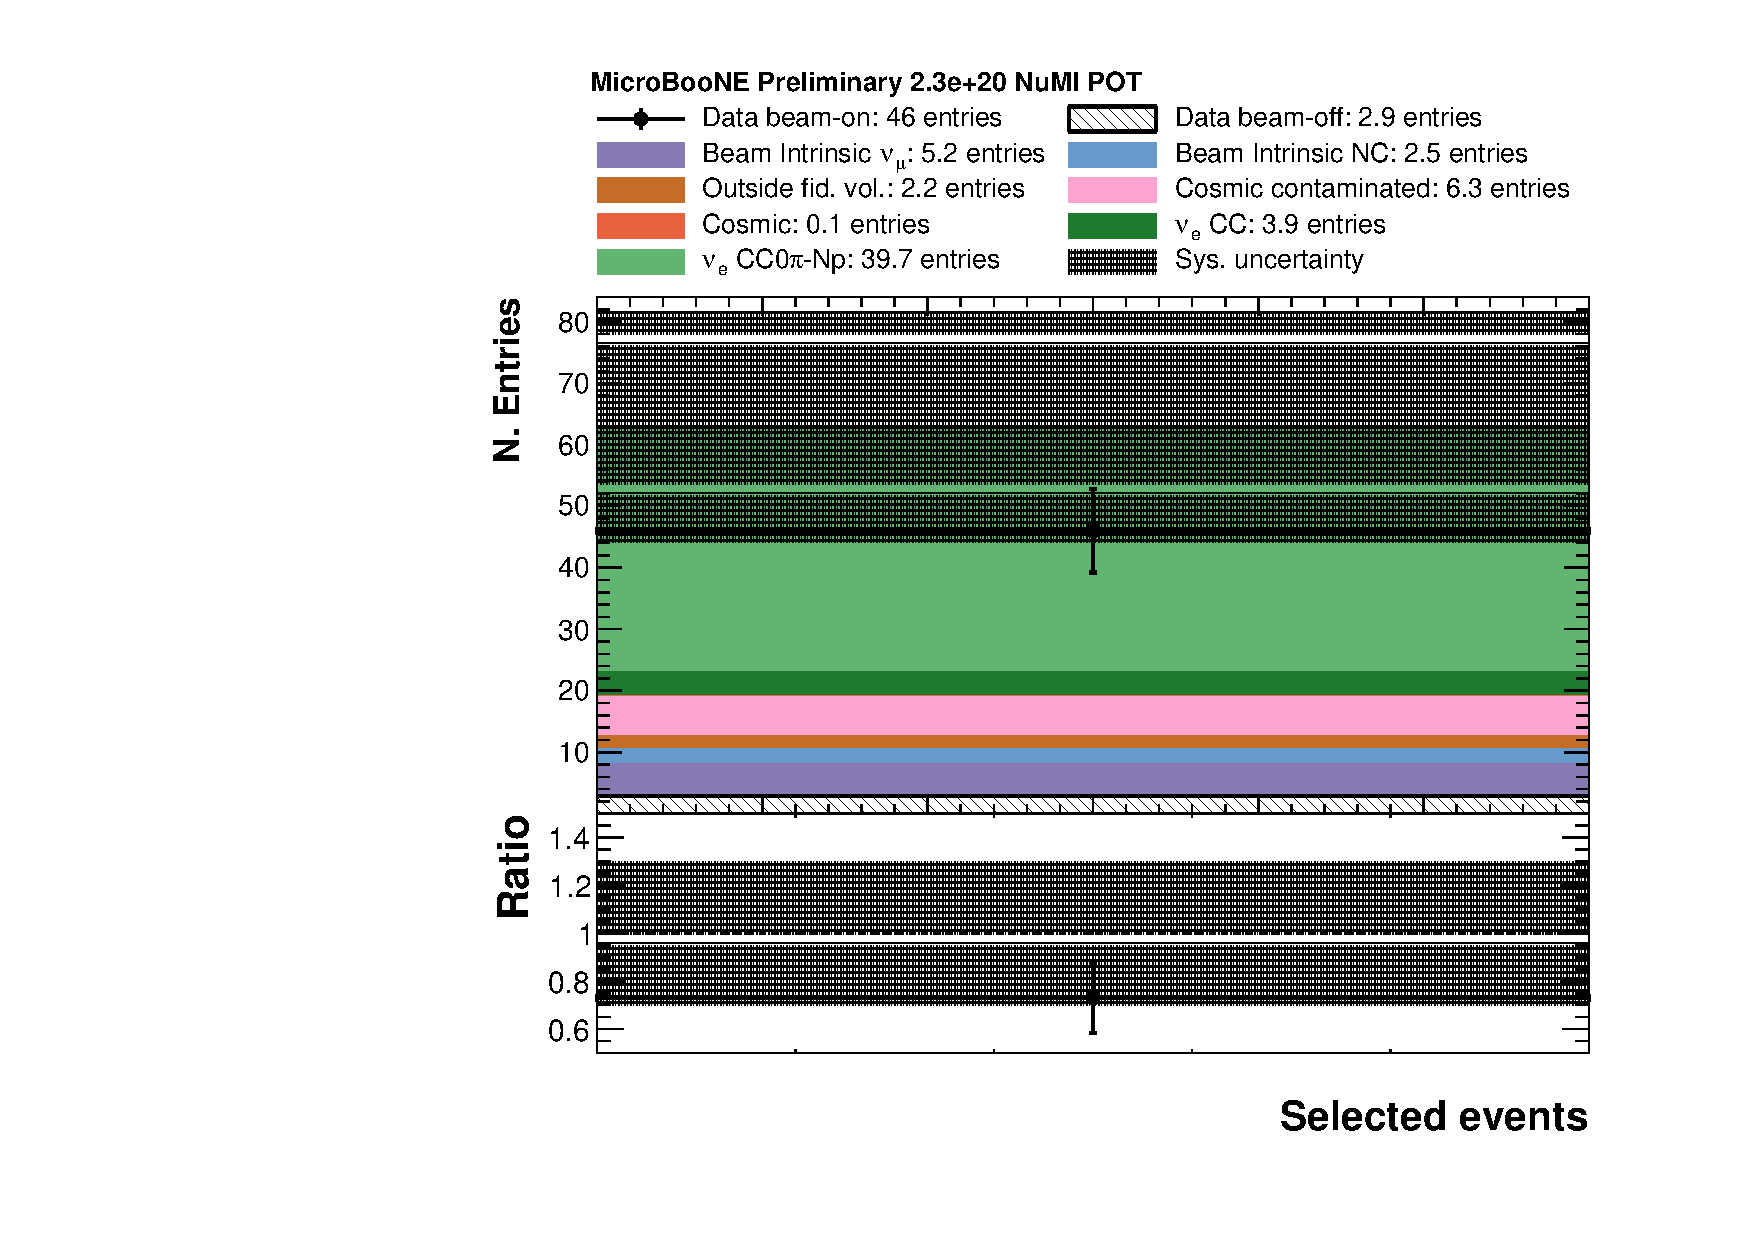
\includegraphics[width=0.75\linewidth]{figures/numi_events.pdf}
  \caption{Number of selected events after the selection and rectangular cuts described in Section \ref{sec:cuts}, plus an additional threshold on the leading shower energy of 100~MeV. The simulated events are classified according to the event category. The number of events corresponds to $2.3\times10^{20}$ NuMI POT in neutrino mode.}\label{fig:numi_nue}
\end{figure}

Figure \ref{fig:numi_nue} shows the number of selected events in data and Monte Carlo for $2.3\times10^{20}$ NuMI POT, collected between February and June 2016 in neutrino mode. Proper systematic uncertainties for NuMI events still need to be assessed, since the off-axis positioning introduces a large uncertainty in the flux that needs to be carefully evaluated. A conservative estimate gives an expected 30\% systematic uncertainty in the number of selected events.

We select 46 data events, $39.7\pm11.9$ signal ($\nu_e$~CC0$\pi$-Np) events, and $23.1\pm6.9$ background events. In order to calculate the significance of the detection of $\nu_e$~CC0$\pi$-Np events, it is necessary to take into account the large size of the signal $s$ with respect to the background $b$. In this case, the usual formula:
\begin{equation}
    \sigma = \frac{s}{\sqrt{b}}
\end{equation}
is not valid. Thus, we adopt a profile-likelihood ratio test, as described in \cite{Cowan:2010js}.
Assuming a 30\% systematic uncertainty, the expected (observed) significance for the detection of $\nu_e$~CC0$\pi$-Np events is 3.4$\sigma$ (2.2$\sigma$). The statistical-only significance is $6.8\sigma$ ($4.2\sigma$).

This result represents a very important cross-check for the analysis, since it gives us confidence that we are indeed selecting $\nu_e$~CC0$\pi$-Np interactions. It also provides a larger sample of electron neutrinos, allowing us to study in detail the shower properties, which will lead to improved cuts and selection efficiencies.
\section{Systematic uncertainties}\label{sec:systematics}
In this analysis, the systematic uncertainties of the quantities described in Section \ref{sec:methodology} can be divided into three main categories: 
\begin{description}
\item[Neutrino generator.] Our Monte Carlo simulation relies on the neutrino generator provided by the GENIE collaboration \cite{Andreopoulos:2009rq}. This generator can be configured to use different physics models, which can affect the relative abundance and the energy of the particles in the final state.
\item[Flux simulation.] The amount of $\nu_{\mu}$ and $\nu_{e}$ reaching the MicroBooNE detector is evaluated by an independent simulation of the neutrino flux of the BNB, used also in the MiniBooNE experiment. This simulation is affected by some uncertainties that need to be taken into account.
\item[Detector simulation.] The detector response (noise removal, signal processing, hit reconstruction) must be carefully simulated in order to achieve a good agreement between data and Monte Carlo in the reconstructed quantities used for background rejection. 
\end{description}

The systematic uncertainties related to the neutrino generator and the flux are evaluated by simulating several \emph{universes}, where the GENIE and flux parameters are varied within their uncertainties. The covariance matrix is defined as:
\begin{equation}
    E_{ij}^{\mathrm{flux, GENIE}} = \frac{1}{N_{u}} \sum^{N_{u}}_{u=0} (x^{u}_{i} - x^{cv}_{i}) (x^{u}_{j} - x^{cv}_{j}),\label{eq:covariance}
\end{equation}
where $i,j$ are the bins of the $x$ reconstructed variable, $N_{u}$ is the number of simulated universes (100 in our case), $x^{u}$ is the reconstructed variable in the $u$ universe and $x^{cv}$ is the central value of the reconstructed variable. 
The detector systematic uncertainties are instead evaluated by varying one parameter per time. In this case, the covariance matrix is:
\begin{equation}
    E_{ij}^{\mathrm{det}} = \sum^{v}_{s=0} (x^{s}_{i} - x^{cv}_{i}) (x^{s}_{j} - x^{cv}_{j}),\label{eq:cov_det}
\end{equation}
where $v$ is the number of detector variations samples and $x^{s}$ is the value of the reconstructed variable in the $s$ sample. The total covariance matrix $E$ is defined as:
\begin{equation}
    E = E^{\mathrm{stat}} + E^{\mathrm{GENIE}} + E^{\mathrm{flux}} + E^{\mathrm{det}},\label{eq:cov_tot}
\end{equation}
where $E^{\mathrm{stat}}$ corresponds to the statistical uncertainty of the Monte Carlo and data off-beam samples, given their limited size. 
The systematic uncertainty for the bin $i$, shown in the plots of Section \ref{sec:methodology}, corresponds to $\sqrt{E_{ii}}$. The fractional covariance matrix $F$ is directly obtained from the covariance matrix and the central values as:
\begin{equation} 
    F_{ij} = \frac{E_{ij}}{x_{i}^{cv} x_{j}^{cv}}.
\end{equation}

\subsection{GENIE systematic uncertainties}
In order to estimate the GENIE systematic uncertainties, the standard GENIE parameters described in \cite{Andreopoulos:2009rq} are simultaneously varied within their uncertainties in $N_{u} = 100$ simulated universes. To each universe it will correspond a \emph{weight}, which is applied when filling the histograms of the reconstructed quantities.

Figure \ref{fig:eff_genie} shows the central value of the $\nu_{e}$ CC0$\pi$-Np selection efficiency and the corresponding value for each GENIE variation universe. The variation in this case is expected to be small, since we are essentially dividing two distributions with the same weight. Figure \ref{fig:reco_genie} and Figure \ref{fig:frac_genie} show that the variations in the reconstructed energy spectrum are larger at lower energies, which is the energy region most affected by the GENIE parameters' uncertainties. The GENIE-related uncertainty in the number of selected events from the BNB+cosmic sample is 7.6\%.


\begin{figure}[htbp]
  \begin{center}
    \begin{subfigure}{0.45\textwidth}
      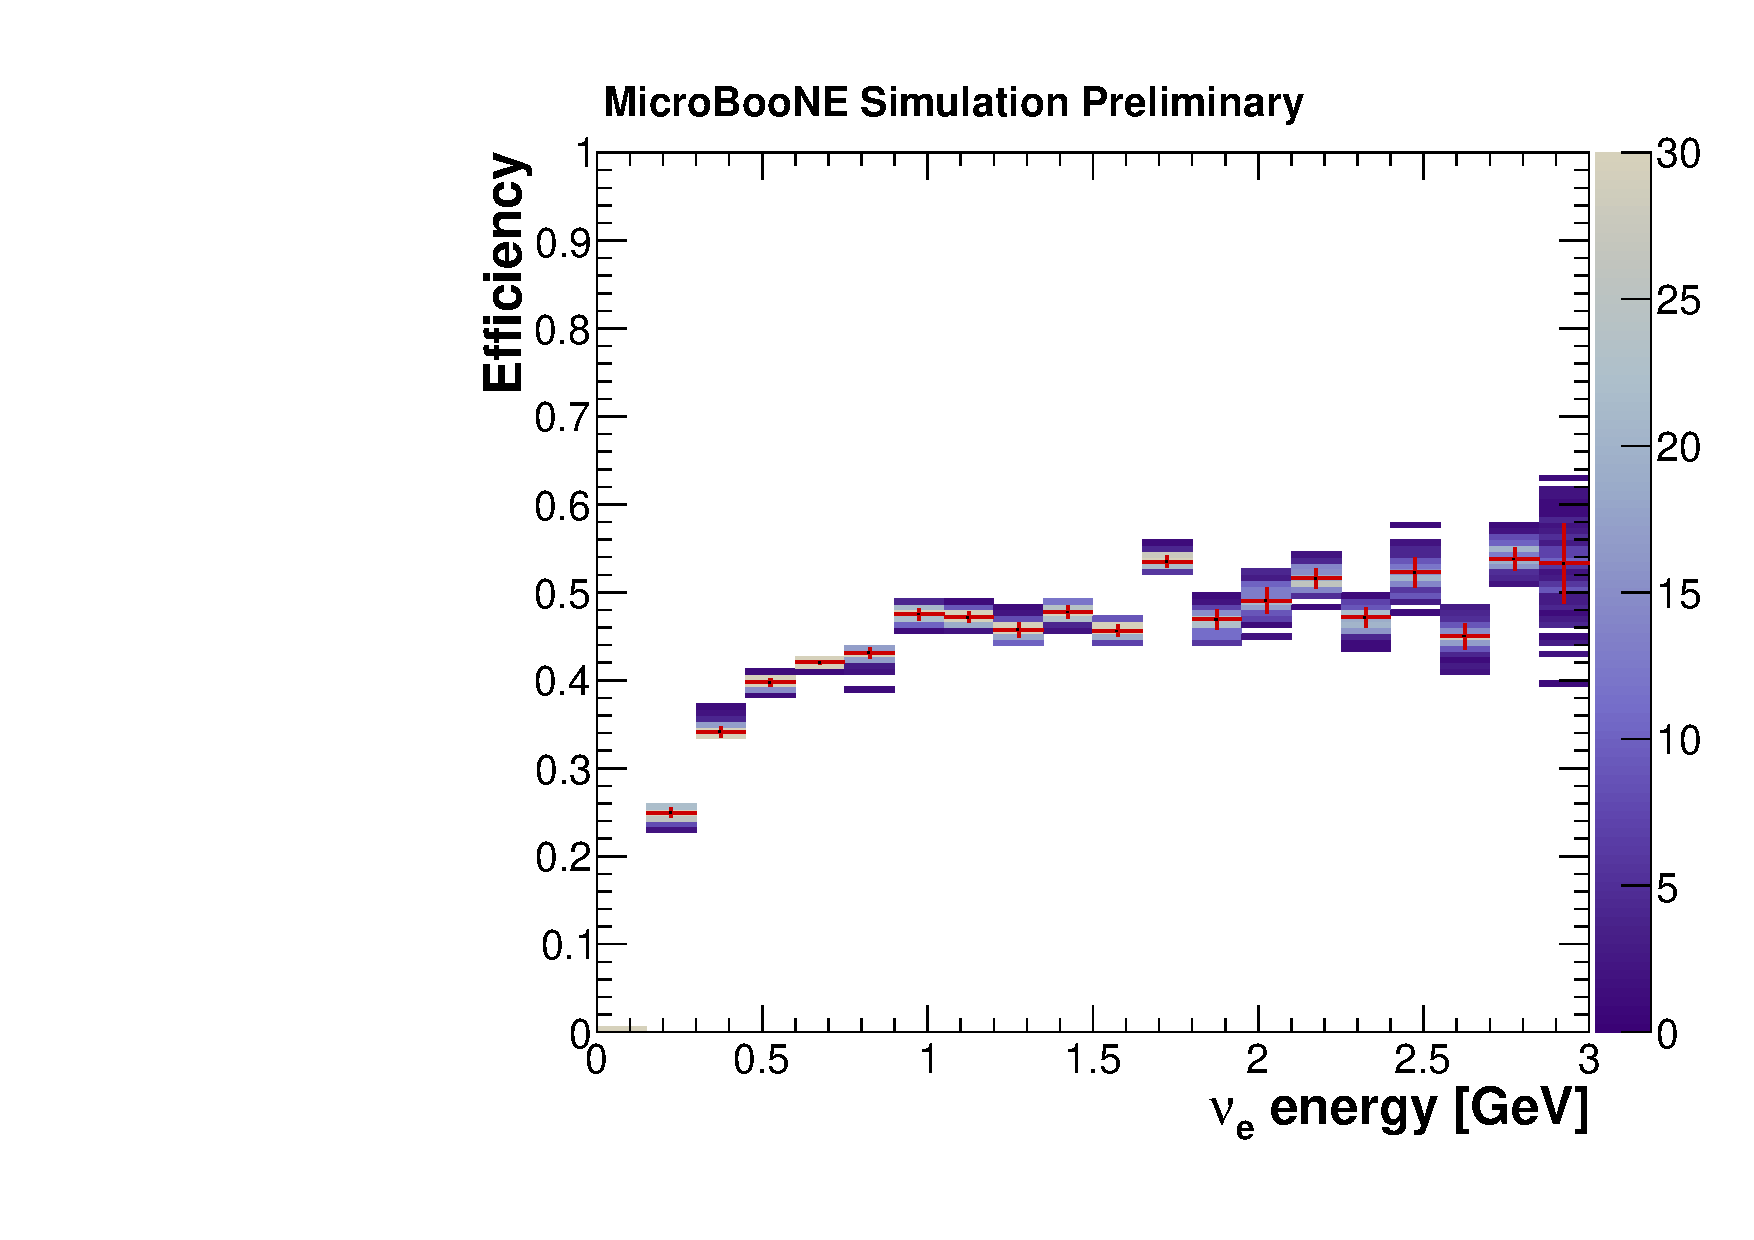
\includegraphics[width=\linewidth]{figures/eff_ene_genie.pdf}
      \caption{$\nu_{e}$ CC0$\pi$-Np selection efficiency.}  \label{fig:eff_genie}
    \end{subfigure}
    \begin{subfigure}{0.45\textwidth}
      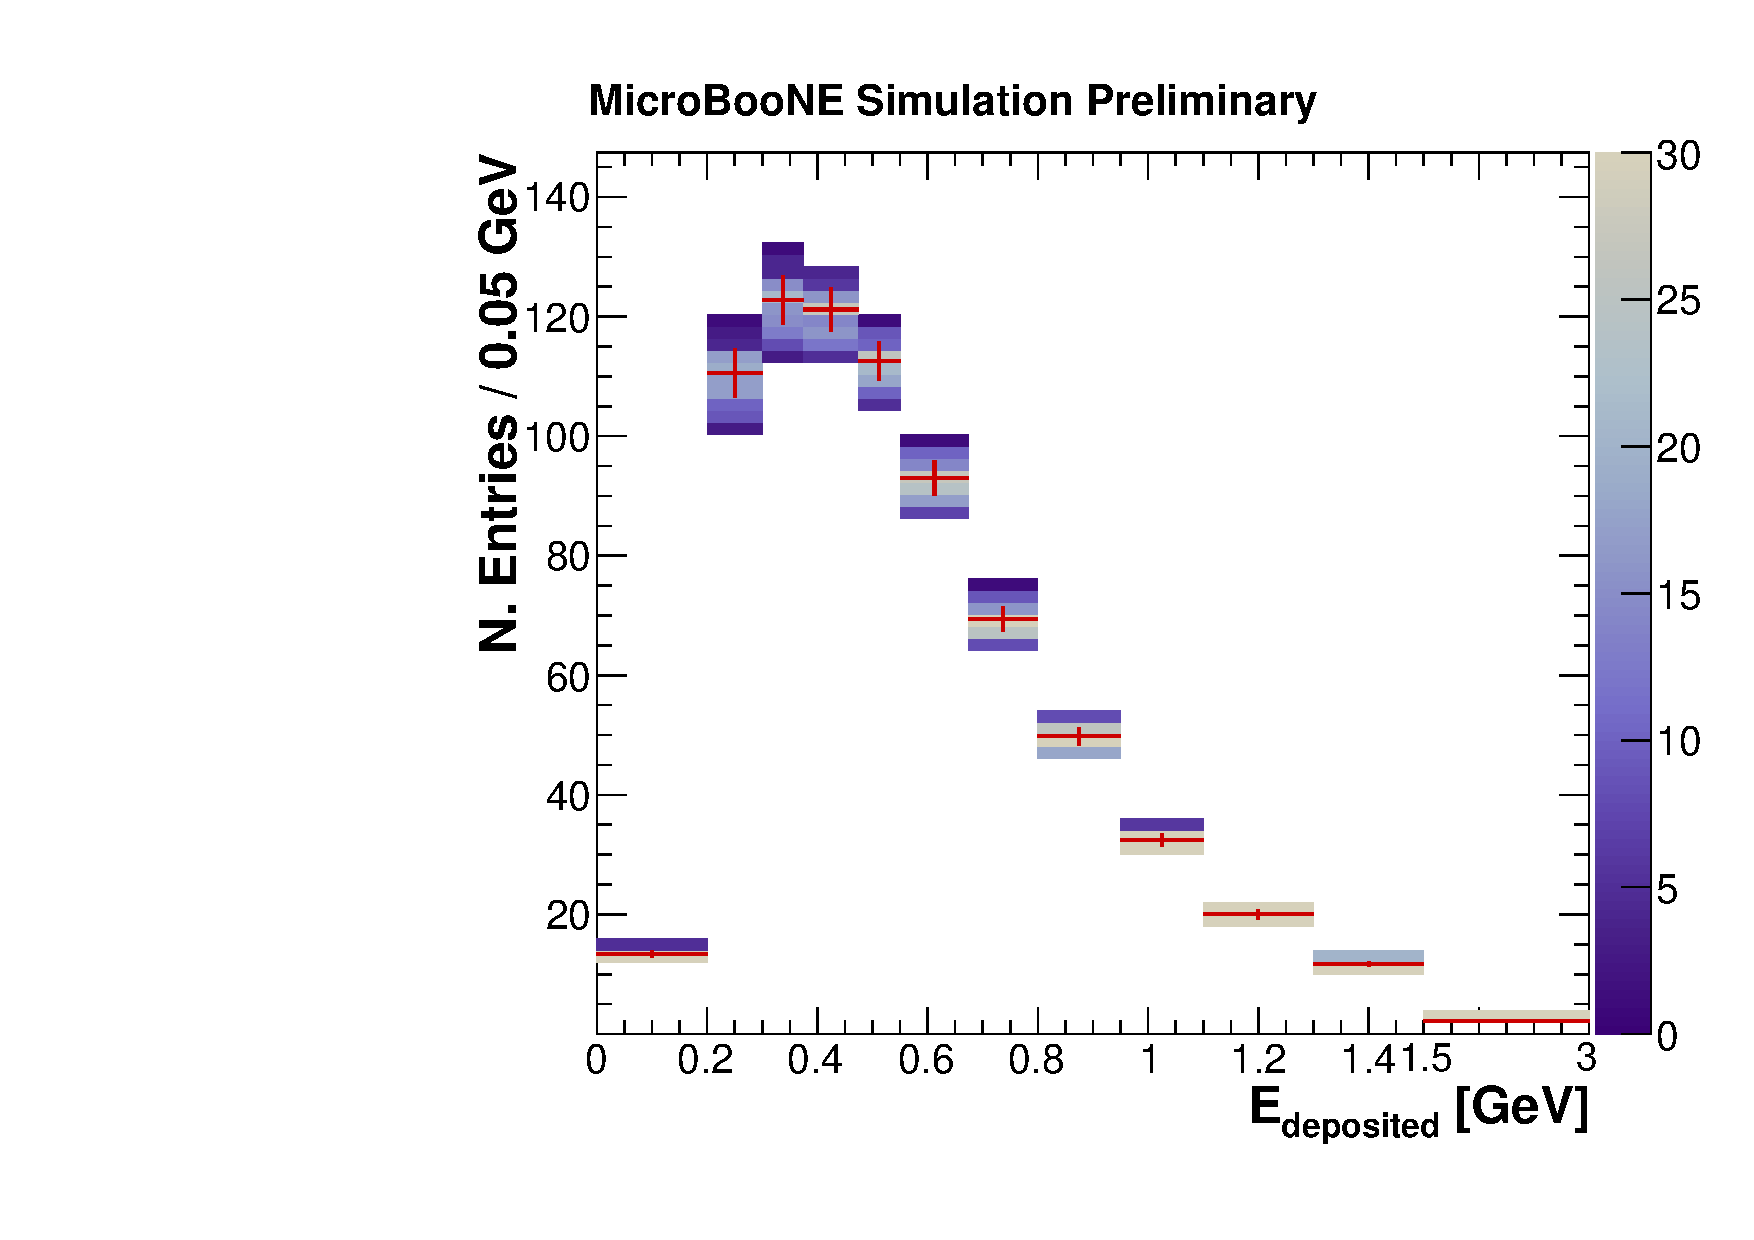
\includegraphics[width=\linewidth]{figures/reco_genie.pdf}
      \caption{$\nu_{e}$ CC0$\pi$-Np candidates energy spectrum in the BNB+cosmic sample.}  \label{fig:reco_genie}
    \end{subfigure}
    \begin{subfigure}{0.45\textwidth}
      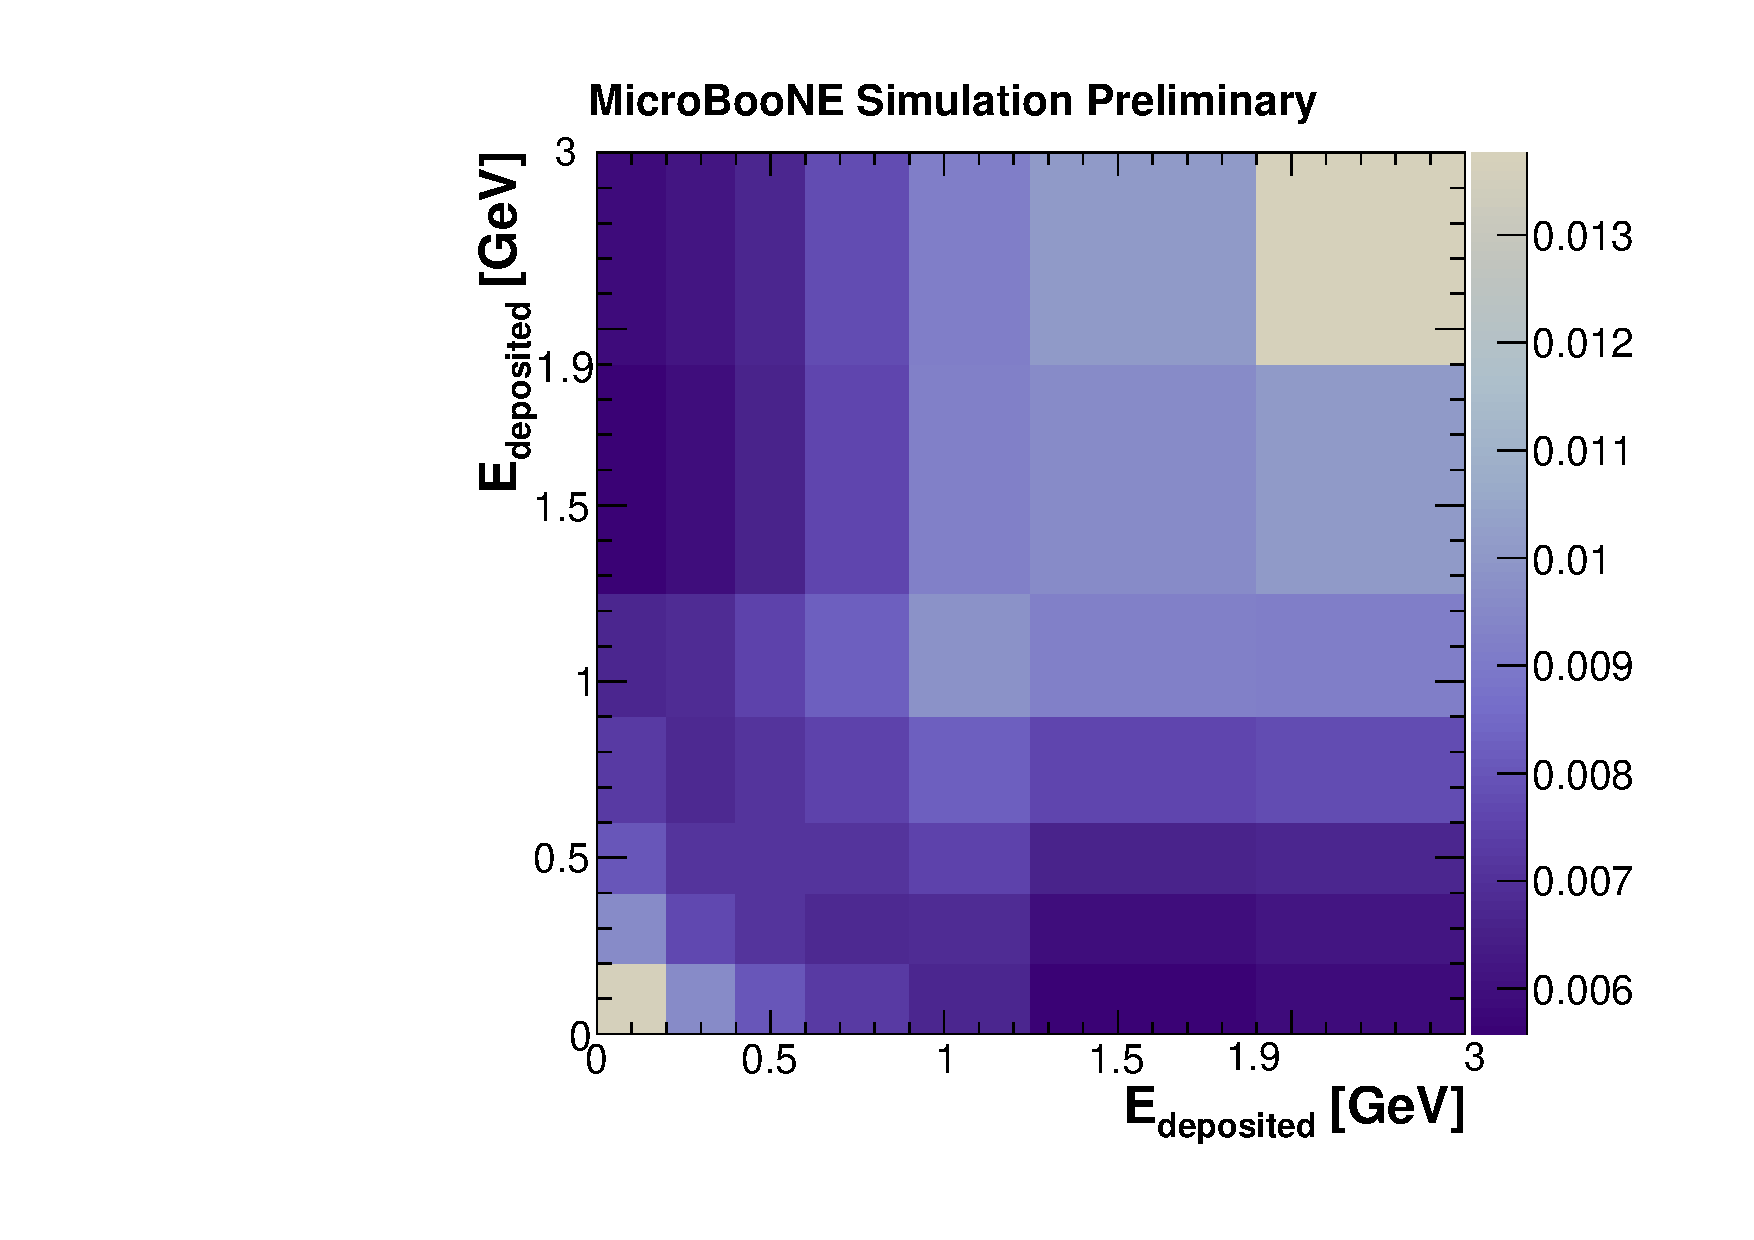
\includegraphics[width=\linewidth]{figures/frac_genie.pdf}
      \caption{GENIE variations fractional covariance matrix.}  \label{fig:frac_genie}
    \end{subfigure}
    	\caption{Selection efficiency, reconstructed energy spectrum, and fractional covariance matrix obtained by varying the standard GENIE parameters in 100 simulated universes. The red bars correspond to the central value and its GENIE systematic uncertainty only.} \label{fig:genie_sys}
	\end{center}
\end{figure}


\subsection{Flux systematic uncertainties}
MicroBooNE is using the same simulation of the BNB flux of the MiniBooNE collaboration. The systematic uncertainties of this simulation, thoroughly described in \cite{AguilarArevalo:2008yp}, can be divided into five main categories:
\begin{description}
\item[Proton delivery:] the numbers of protons hitting the target is affected by the uncertainties in the proton beam optics, which in turns affects the amount of neutrinos in the beam.
\item[Particle production]. The rate and spectrum of secondary particles in the interaction between the protons and the beryllium (the target material) affects the rate and spectrum of the neutrinos. This is main uncertainty in the flux simulation \cite{AguilarArevalo:2008yp}.
\item[Hadronic interactions:] the rate and shape of the flux is affected by the rate of hadronic interactions and the hadronic survival probability both in the target and in the horn.
\item[Horn magnetic field:] uncertainties in the distribution of the magnetic field affect the spectrum of the neutrino flux.
\item[Beamline geometry:] misalignments or displacements of the beamline with respect to the detector can affect the relative neutrino flavour abundances and the flux rate.
\end{description}

In this analysis, the systematic uncertainties related to the flux simulation are evaluated by generating 100 universes, where the flux parameters are varied within their uncertainties. 

Figure \ref{fig:eff_flux} shows the central value of the $\nu_{e}$ CC0$\pi$-Np selection efficiency and the corresponding value for each flux variation universe. Also here, the variation in the efficiency is small, as expected. Figure \ref{fig:reco_flux} shows a bias of the variation samples with respect to the nominal simulation, which does not correspond to the average of the universes. This is caused by an inconsistency of the pion production cross-section used in the generation of the universes \cite{ubxsec}. In this case, the nominal value is considered as the central value in the covariance matrix definition \eqref{eq:covariance}. The flux-related uncertainty in the number of selected events from the BNB+cosmic sample is 7.8\%.

\begin{figure}[htbp]
  \begin{center}
    \begin{subfigure}{0.45\textwidth}
      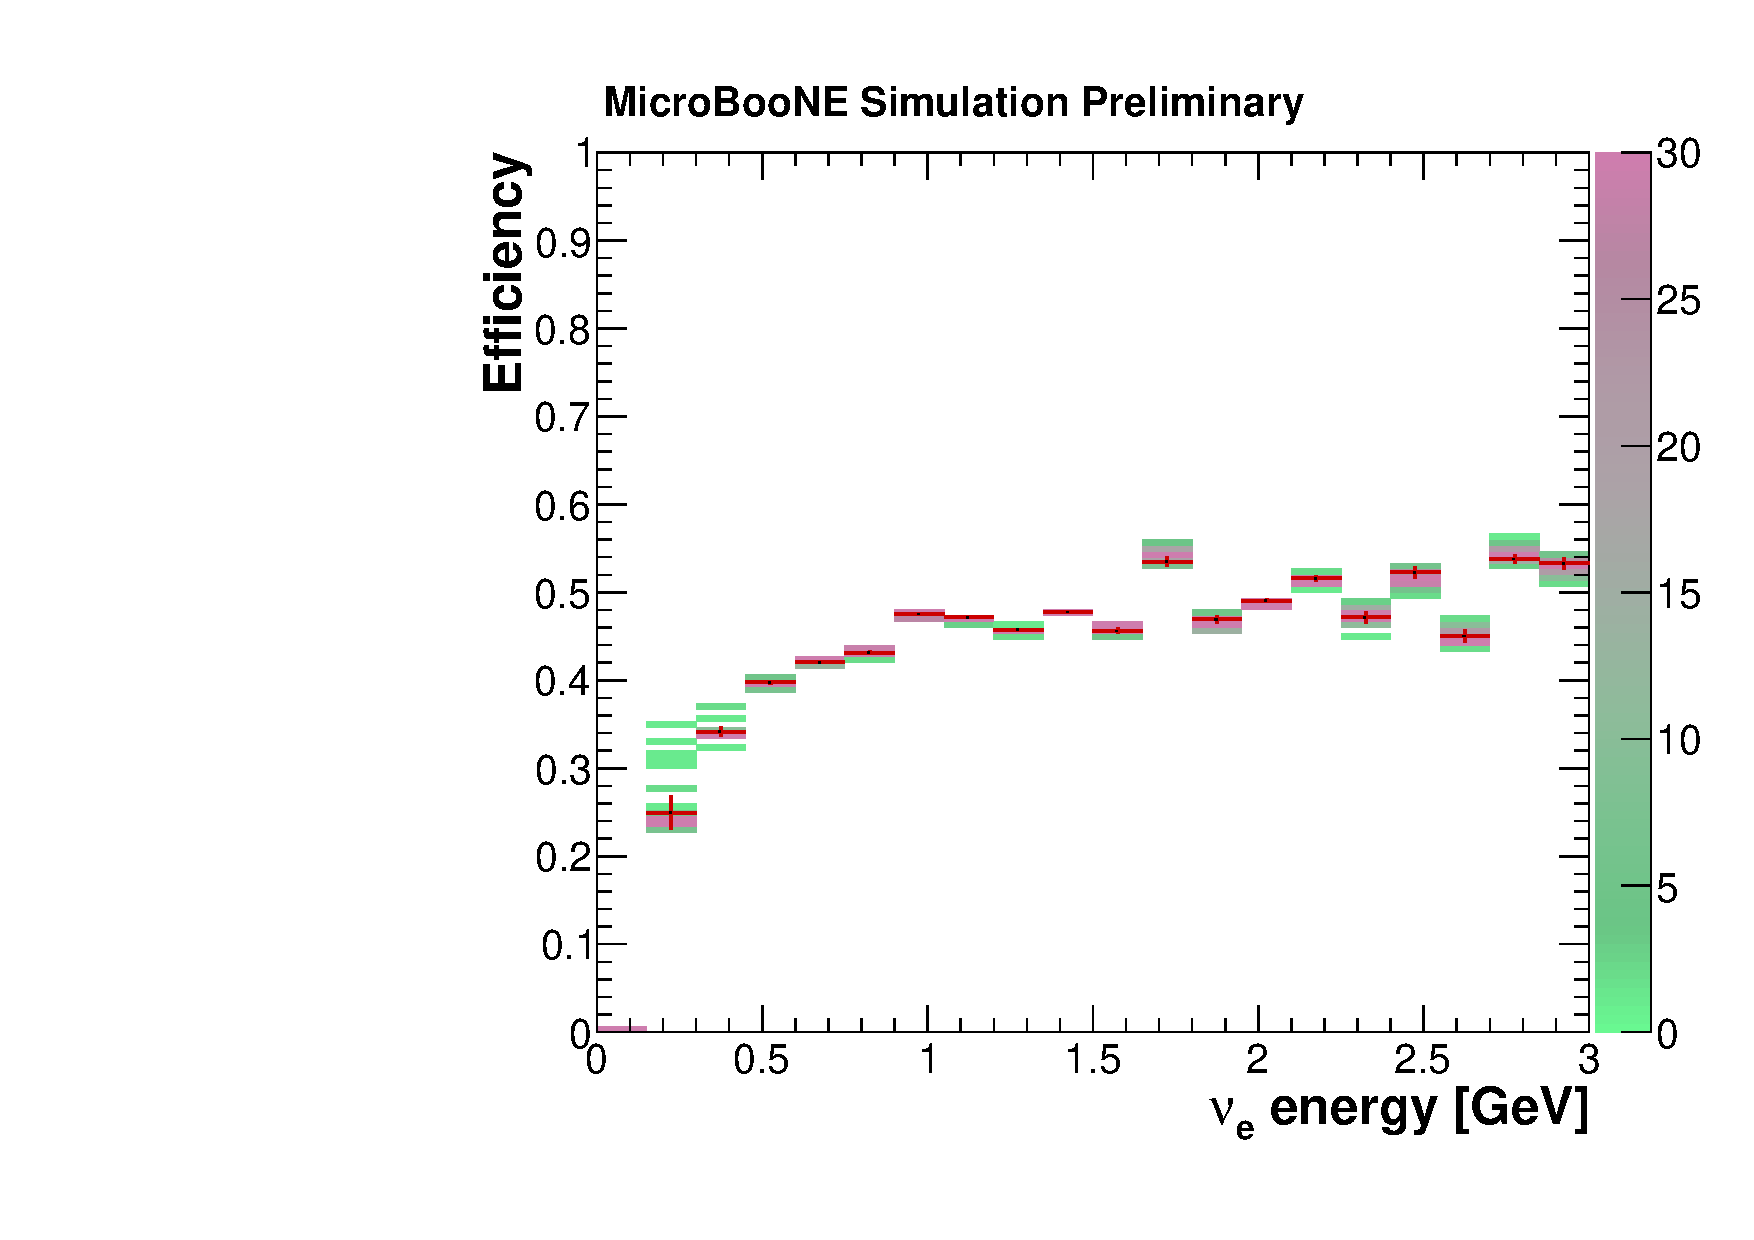
\includegraphics[width=\linewidth]{figures/eff_ene_flux.pdf}
      \caption{$\nu_{e}$ CC0$\pi$-Np selection efficiency.}  \label{fig:eff_flux}
    \end{subfigure}
    \begin{subfigure}{0.45\textwidth}
      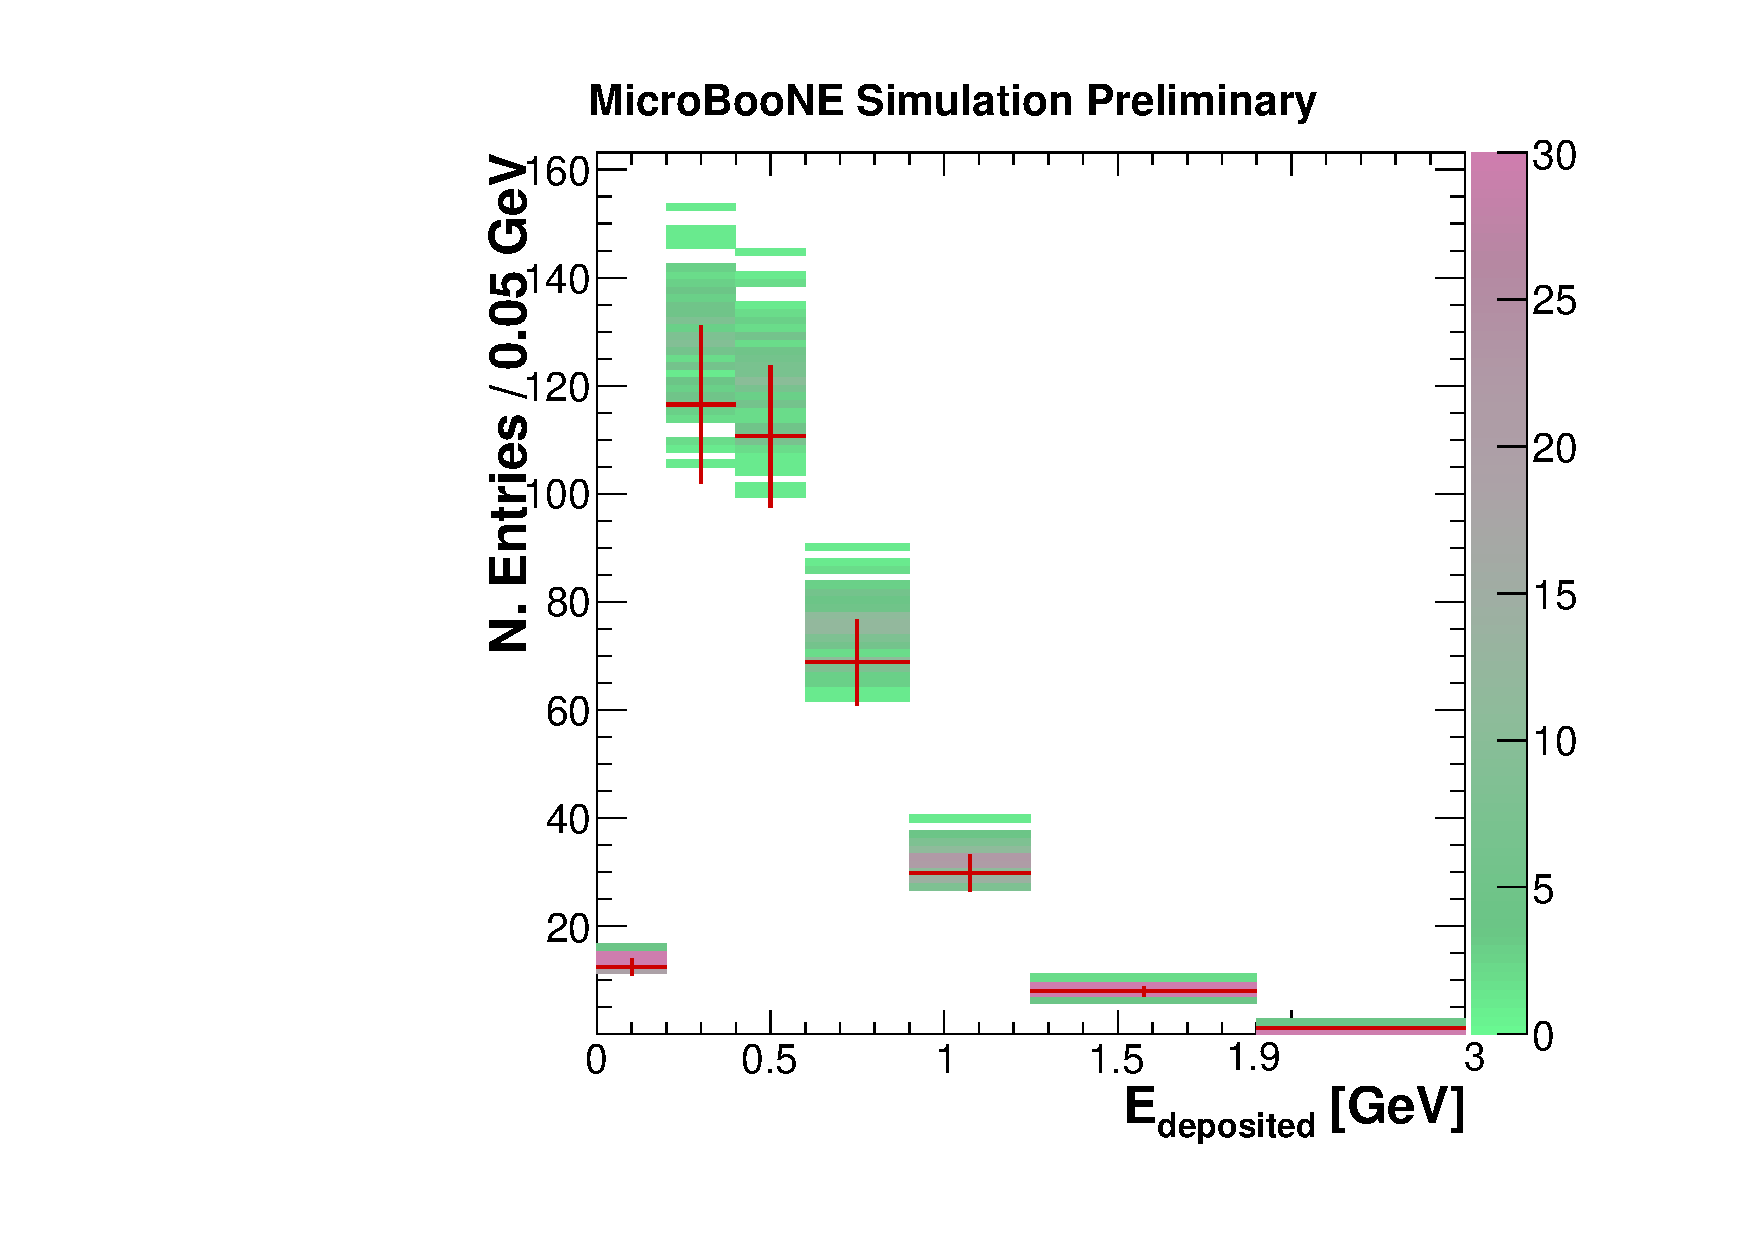
\includegraphics[width=\linewidth]{figures/reco_flux.pdf}
      \caption{$\nu_{e}$ CC0$\pi$-Np candidates energy spectrum in the BNB+cosmic sample.}  \label{fig:reco_flux}
    \end{subfigure}
    \begin{subfigure}{0.45\textwidth}
      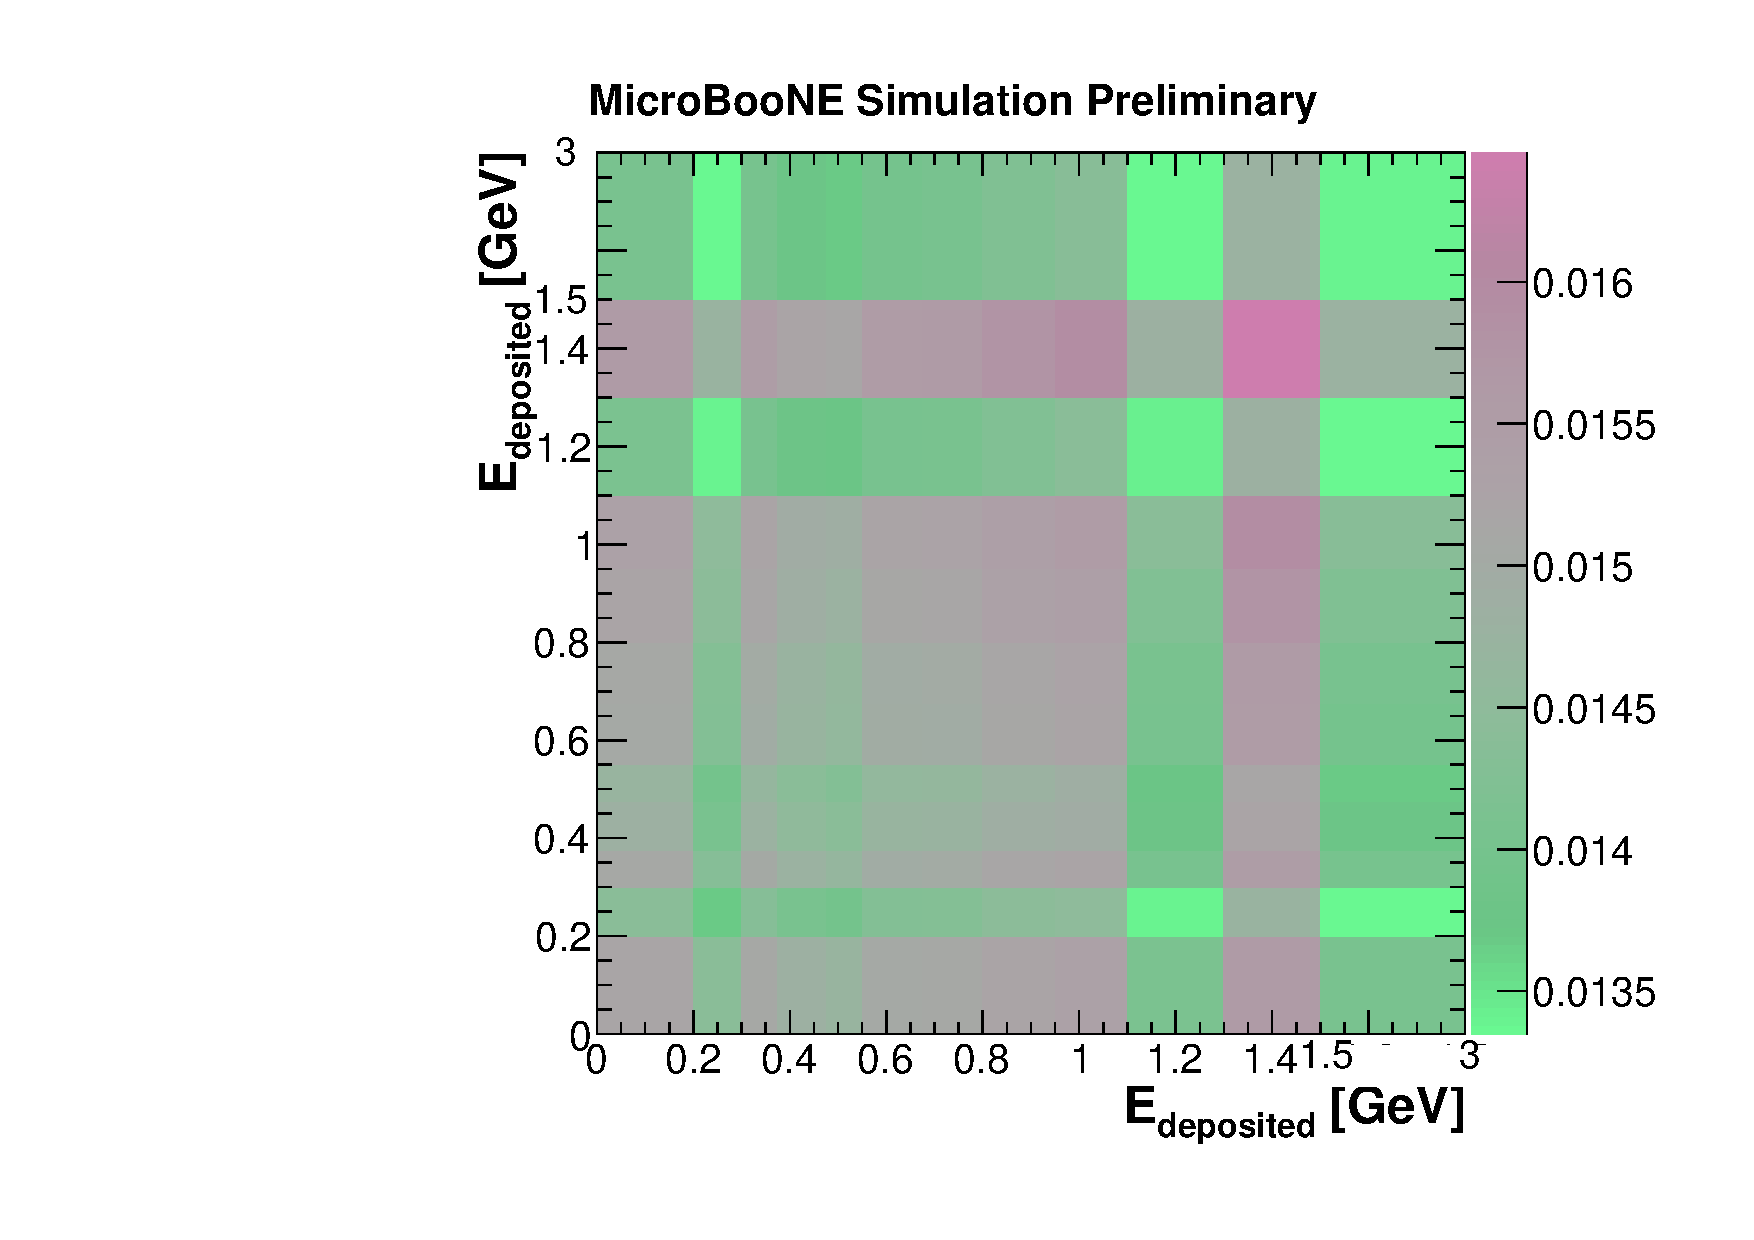
\includegraphics[width=\linewidth]{figures/frac_flux.pdf}
      \caption{Flux variations fractional covariance matrix.}  \label{fig:frac_flux}
    \end{subfigure}
    	\caption{Selection efficiency, reconstructed energy spectrum, and fractional covariance matrix obtained by varying the BNB flux parameters in 100 simulated universes.  The red bars correspond to the central value and its flux systematic uncertainty only.} \label{fig:flux_sys}
	\end{center}
\end{figure}

\subsection{Detector systematic uncertainties}
The detector systematic uncertainties have been measured by simulating several samples where a single detector parameter is varied by its uncertainty or a different physics model is used. In this case, the covariance matrix is evaluated using the definition in eq. \eqref{eq:cov_det}. The fractional covariance matrix and the reconstructed energy spectrum are shown in Figure \ref{fig:frac_det} and Figure \ref{fig:reco_det}, respectively.
The uncertainty related to the detector systematic effects in the number of selected events from the BNB+cosmic sample is 21.9\%. Given the limited size of the detector variation samples, a flat 21.9\% uncertainty is applied to the BNB+cosmic component of the $\nu_{\mu}$ and NC-enhanced samples.

\begin{figure}[htbp]
  \begin{center}
    \begin{subfigure}{0.45\textwidth}
      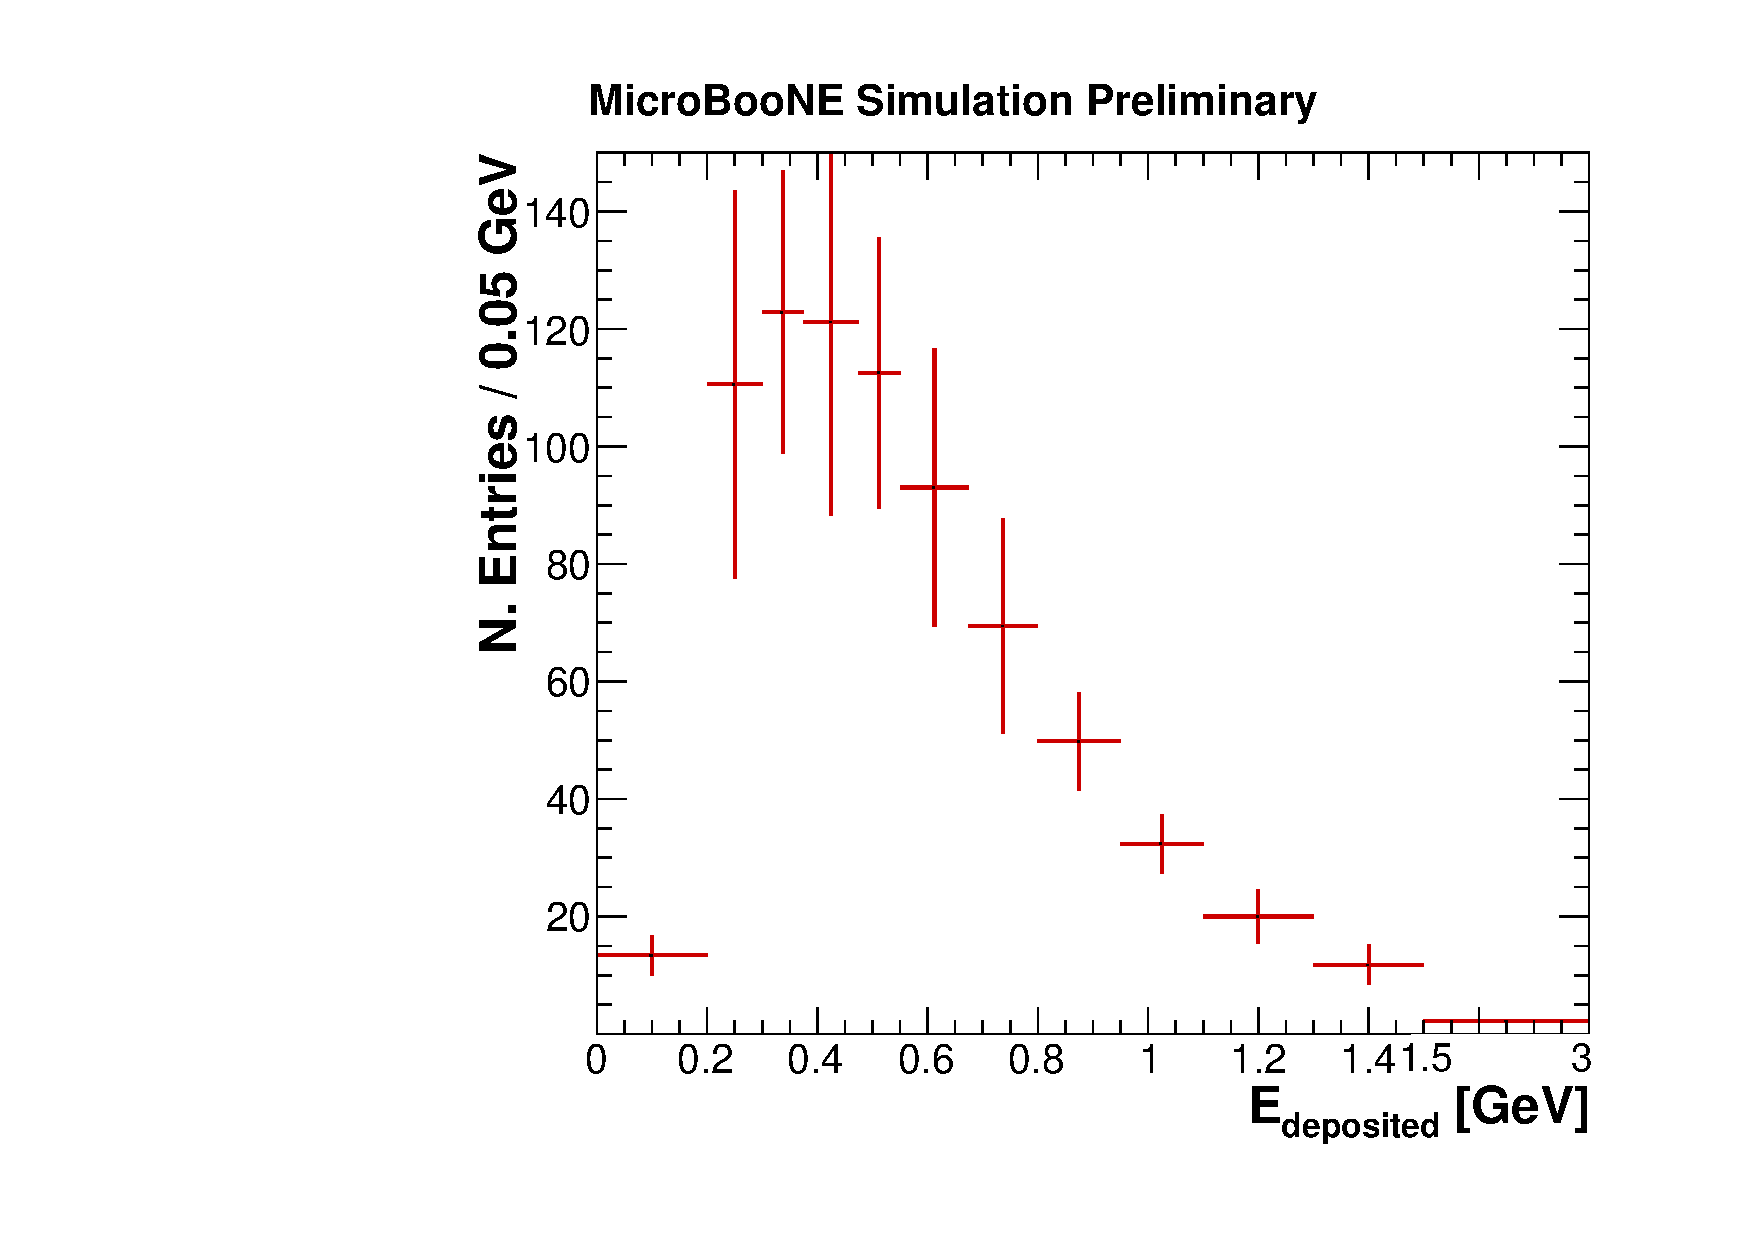
\includegraphics[width=\linewidth]{figures/reco_det.pdf}
      \caption{$\nu_{e}$ CC0$\pi$-Np candidates energy spectrum in the BNB+cosmic sample.}  \label{fig:reco_det}
    \end{subfigure}
    \begin{subfigure}{0.45\textwidth}
      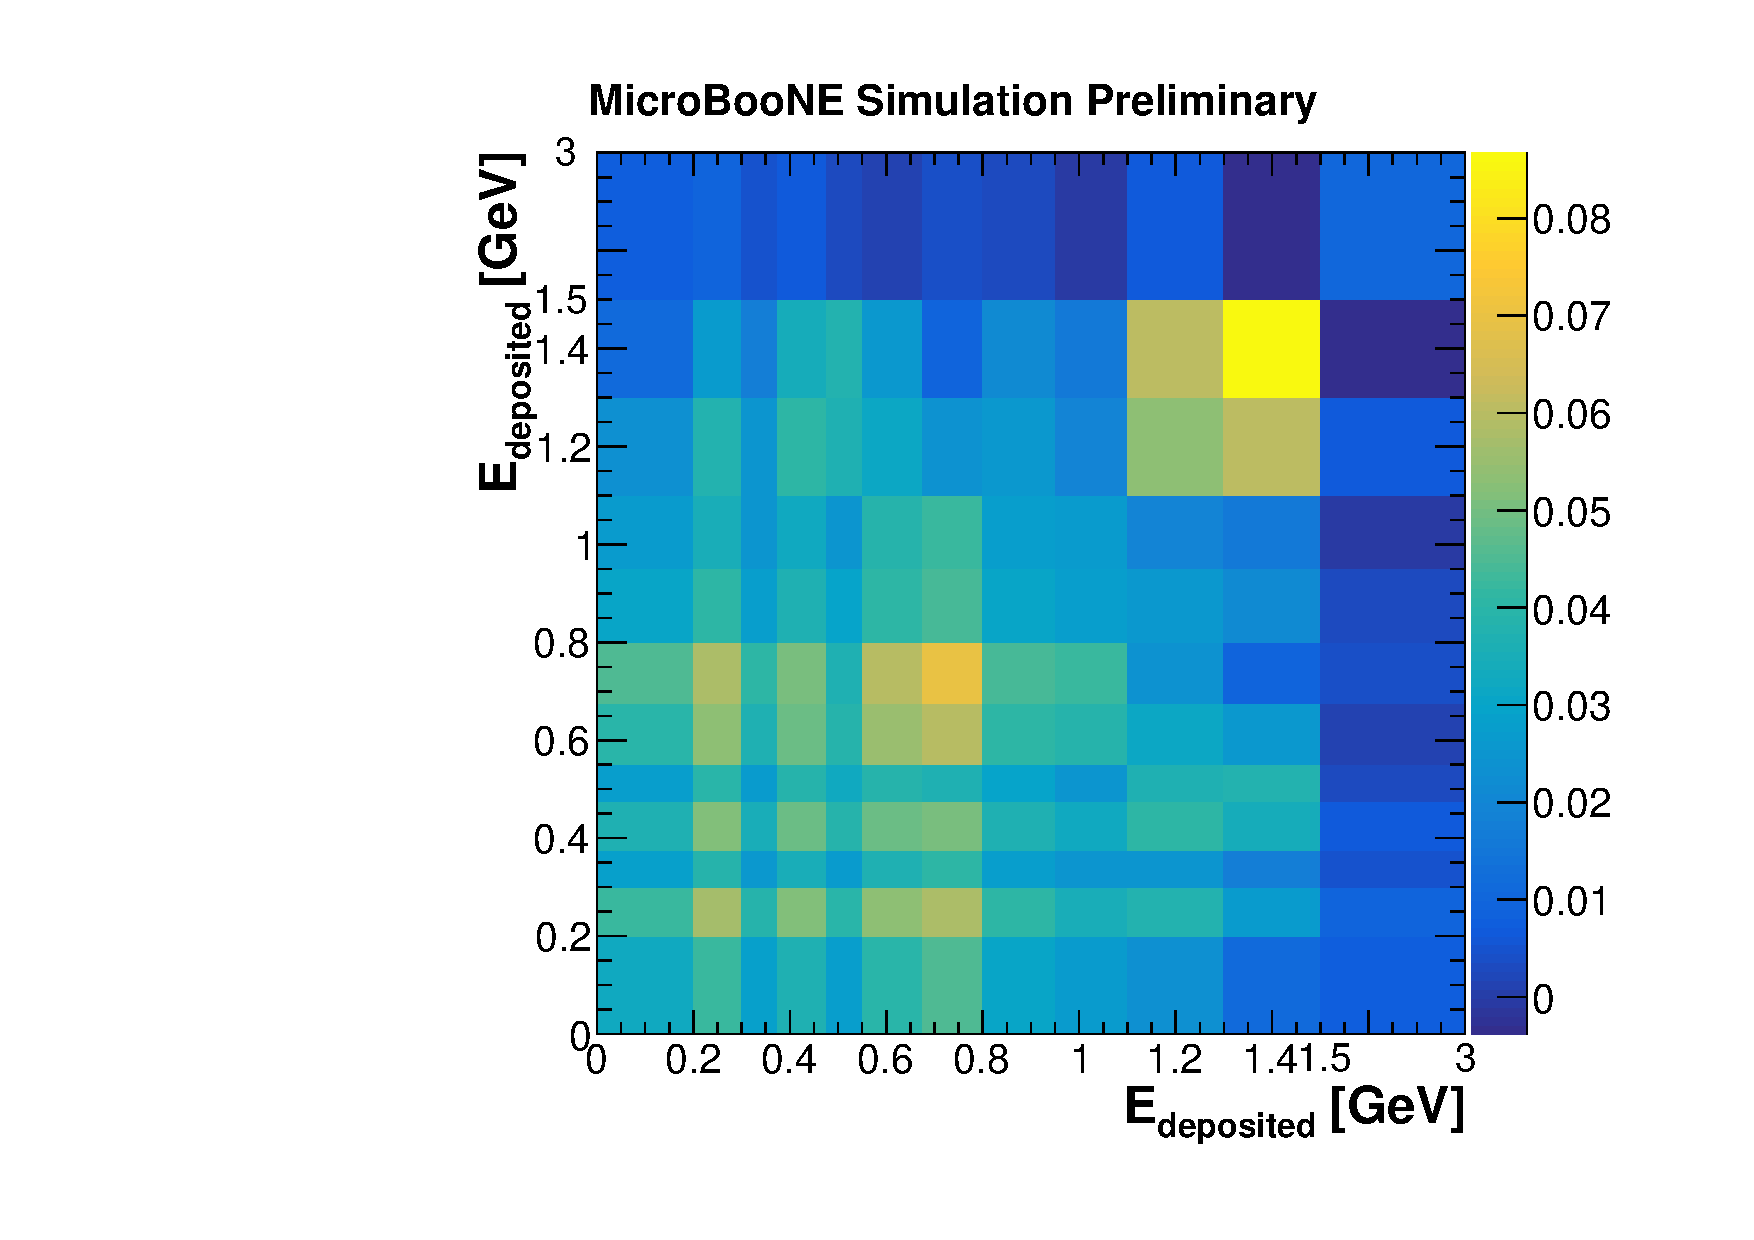
\includegraphics[width=\linewidth]{figures/frac_det.pdf}
      \caption{Detector variations fractional covariance matrix.}  \label{fig:frac_det}
    \end{subfigure}
    	\caption{Reconstructed energy spectrum, and fractional covariance matrix obtained with the detector variations samples.  The red bars correspond to the central value and its detector systematic uncertainty only.} \label{fig:det_sys}
	\end{center}
\end{figure}


\vspace{1em}
Table \ref{tab:syst} shows the uncertainty in the number of selected events from in the BNB+cosmic sample for the GENIE, flux, and detector systematic variations. The total uncertainty, obtained with eq. \ref{eq:cov_tot}, is 21.9~\%. In the POT-normalized figures of Section \ref{sec:methodology}, the uncertainty on the dirt and the $\nu_{e}$ CC$0\pi$-Np samples is assumed to be the same one of the BNB+cosmic sample. Given the small contribution of these samples to the number of selected events (2.5\% of the total), this approximation is considered good enough at this stage. The statistical uncertainty of the data off-beam sample is 1.0\%. 

\begin{table}[htbp]
\footnotesize{
   \centering
   \begin{tabular}{p{0.23\linewidth}p{0.33\linewidth}p{0.21\linewidth}p{0.11\linewidth}}
     \toprule
     Type & Description & Method & Uncertainty \\
     \midrule
     Monte Carlo statistics & Finite size of the Monte Carlo sample. & - & 1.9~\%\\
     GENIE & Variations of the neutrino generator parameters within their uncertainties. & 100 universes & 7.6~\%\\
     Flux & Variations of the flux simulation parameters within their uncertainties. & 100 universes & 7.8~\%\\
     Space-charge effect & Data-driven estimation of the space-charge effect. & Alternate simulation & 9.7~\%\\
     Dynamic Induced Charge & Improved simulation of the induction of charge on the wires. & Alternate simulation & 9.5~\%\\
     Light simulation & Improved simulation of the light production in the detector. & Alternate simulation & 4.0~\%\\
     Saturated channels & Channels that tends to saturate are turned off in the simulation. & Alternate simulation & 4.2~\%\\
     Misconfigured channels & Channels with misconfigured ASIC gains and shaping are turned off in the simulation. & Alternate simulation & 4.1~\%\\
     Electron lifetime & Lifetime of the electron in the detector is reduced to 10~ms. & Alternate model & 3.9~\%\\
     Recombination model & The Birks model of recombination \cite{Amoruso:2004dy} is used instead of the modified box model \cite{Acciarri:2013met}. & Alternate model & 4.0~\%\\
     Longitudinal diffusion & The longitude diffusion is varied within the uncertainty. & $\pm1\sigma$ variation & 4.5~\%\\
     Transverse diffusion & The transverse diffusion is varied within the uncertainty. & $\pm1\sigma$ variation & 4.8~\%\\
     Wire noise & The amount of noise on the wires is varied within the uncertainty. & $\pm1\sigma$ variation & 3.7~\%\\
     PE noise & The amount of single-PE noise in the PMTs is varied within the uncertainty. & $\pm1\sigma$ variation & 4.8~\%\\
     Cryostat light & The light outside the TPC but inside the cryostat is increased by 50\% & Alternate simulation & 3.8~\%\\
     \midrule
     Total & & & 21.9~\%\\
     \bottomrule
   \end{tabular}
   \caption{Summary of the systematic uncertainties in the number of selected events in the BNB+cosmic sample.}\label{tab:syst}
}
\end{table}

